\subsection{\nogloxy{Premi::Front-End}}
\label{\nogloxy{Premi::Front-End}}
\subsubsection{Informazioni generali}
\begin{figure}[h]
\centering
\nogloxy{\includegraphics[scale=0.4,keepaspectratio]{diagrammi/package/{frontEnd}.pdf}}
\caption{\nogloxy{Premi::Front-End}}
\end{figure}
\FloatBarrier
\begin{itemize}
\item \textbf{Descrizione}\\
Package contenente le varie componenti della parte \gloxy{front end} dell'applicazione.
\item \textbf{Package contenuti}:
\begin{itemize}
\item \hyperref[\nogloxy{Premi::Front-End::Controllers}]{\nogloxy{\texttt{Controllers}}}\\
Package contenente i \gloxy{controller} della componente \gloxy{front-end} dell’applicazione.
\item \hyperref[\nogloxy{Premi::Front-End::Directives}]{\nogloxy{\texttt{Directives}}}\\
Package contenente le directives che compongno le views.
\item \hyperref[\nogloxy{Premi::Front-End::Model}]{\nogloxy{\texttt{Model}}}\\
Package contenente le classi che definiscono la \gloxy{business logic} dell’applicazione.
\item \hyperref[\nogloxy{Premi::Front-End::Services}]{\nogloxy{\texttt{Services}}}\\
Package contenente le classi che descrivono il meccanismo con cui il \gloxy{front-end} può interfacciarsi con le \gloxy{API} \gloxy{REST} del \gloxy{back-end}. Permette di popolare il model del \gloxy{client} e di richiedere l'esecuzione di operazioni al \gloxy{server}.
\item \hyperref[\nogloxy{Premi::Front-End::Views}]{\nogloxy{\texttt{Views}}}\\
Package contenente le views della componente \gloxy{front-end} dell’applicazione.
\end{itemize}
\end{itemize}
\subsubsection{Classi}
\subsubsubsection{\nogloxy{Premi::Front-End::AppConfig}}
\label{\nogloxy{Premi::Front-End::AppConfig}}
\begin{figure}[h]
\centering
\nogloxy{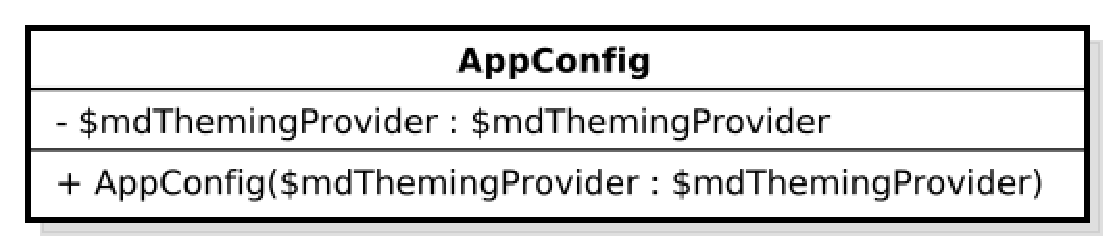
\includegraphics[scale=0.4,keepaspectratio]{diagrammi/classi/{frontEnd/AppConfig}.pdf}}
\caption{\nogloxy{Premi::Front-End::AppConfig}}
\end{figure}
\FloatBarrier
\begin{itemize}
\item \textbf{Descrizione}\\
Classe che si occupa di definire la configurazione dell'applicazione.
\item \textbf{Utilizzo}\\
Viene utilizzata per definire lo schema di colori per l'applicazione.
\item \textbf{Attributi}:
\begin{itemize}
\item \nogloxy{\texttt{- \$mdThemingProvider: \$mdThemingProvider}}
\\ Campo dati contenente un riferimento al servizio della \gloxy{libreria} \nogloxy{\textit{Material for Angular}} che permette di definire lo schema colori dell'applicazione.
\end{itemize}
\item \textbf{Metodi}:
\begin{itemize}
\item \nogloxy{\texttt{+ AppConfig(\$mdThemingProvider: \$mdThemingProvider)}}
\\ \dpConstructor \\ Viene utilizzato per impostare i colori di default dell'applicazione.
\\ \textbf{Parametri}:
\begin{itemize}
\item \nogloxy{\texttt{\$mdThemingProvider: \$mdThemingProvider}}
\\ Parametro contenente un riferimento al servizio della \gloxy{libreria} \nogloxy{\textit{Material for Angular}} che permette di definire lo schema colori dell'applicazione.
\end{itemize}
\end{itemize}
\end{itemize}
\subsubsubsection{\nogloxy{Premi::Front-End::AppRouter}}
\label{\nogloxy{Premi::Front-End::AppRouter}}
\begin{figure}[h]
\centering
\nogloxy{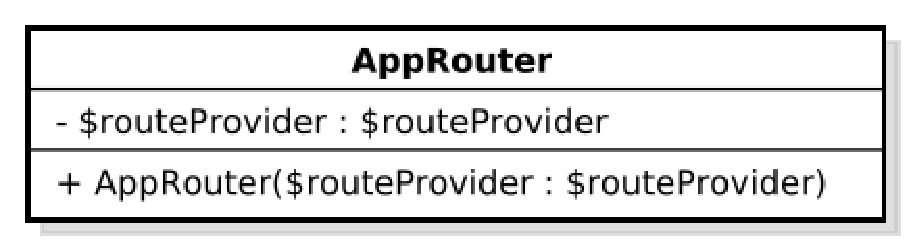
\includegraphics[scale=0.4,keepaspectratio]{diagrammi/classi/{frontEnd/AppRouter}.pdf}}
\caption{\nogloxy{Premi::Front-End::AppRouter}}
\end{figure}
\FloatBarrier
\begin{itemize}
\item \textbf{Descrizione}\\
Classe che gestisce i routes dell'applicazione, utilizza il servizio \texttt{\$routeProvider} per associare ad ogni route un \gloxy{controller} e una \gloxy{view}.
\item \textbf{Utilizzo}\\
Viene utilizzata per associare un URL alle varie \gloxy{view} dell'applicazione.
\item \textbf{Attributi}:
\begin{itemize}
\item \nogloxy{\texttt{- \$routeProvider: \$routeProvider}}
\\ Campo dati contenente un riferimento al servizio di \gloxy{Angular} che si occupa di definire le route per l'applicazione.
\end{itemize}
\item \textbf{Metodi}:
\begin{itemize}
\item \nogloxy{\texttt{+ AppRouter(\$routeProvider: \$routeProvider)}}
\\ \dpConstructor
\\ \textbf{Parametri}:
\begin{itemize}
\item \nogloxy{\texttt{\$routeProvider: \$routeProvider}}
\\ Parametro contenente un riferimento al servizio di \gloxy{Angular} che si occupa di definire le route per l'applicazione.
\end{itemize}
\end{itemize}
\end{itemize}
\subsubsubsection{\nogloxy{Premi::Front-End::AppRun}}
\label{\nogloxy{Premi::Front-End::AppRun}}
\begin{figure}[h]
\centering
\nogloxy{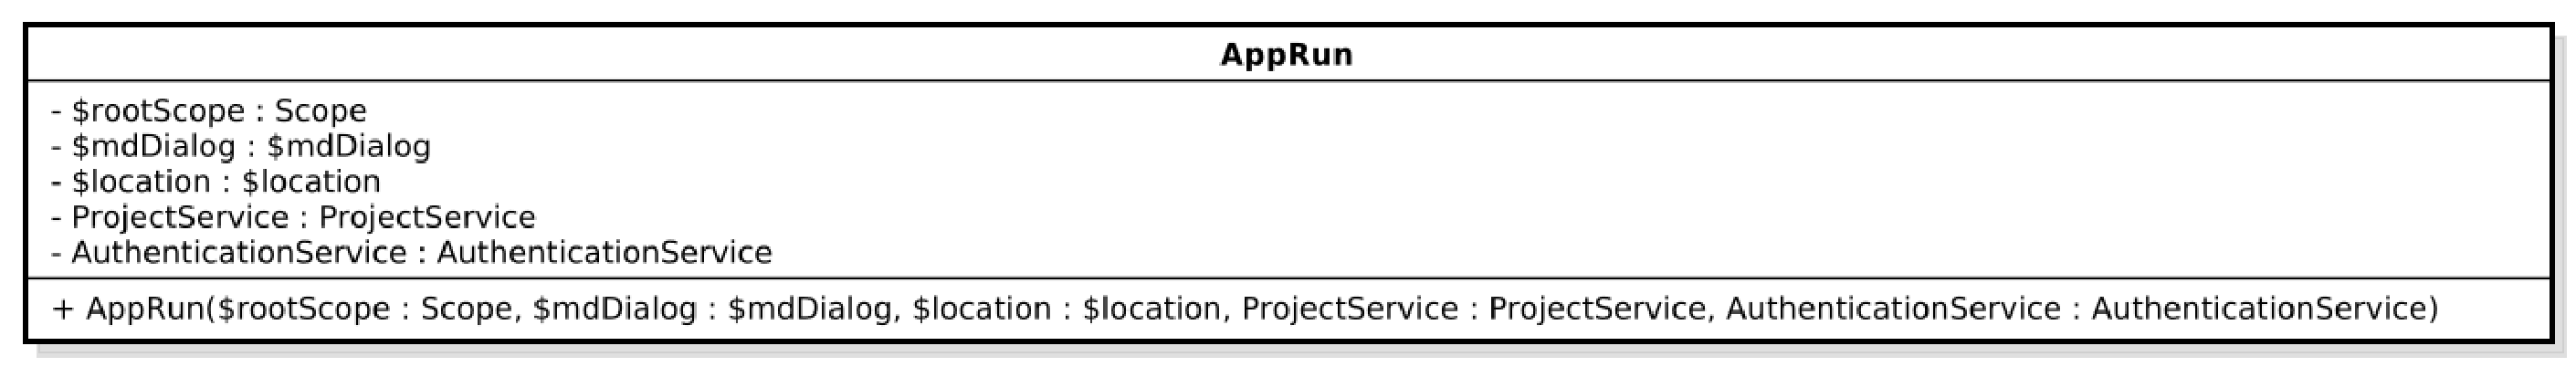
\includegraphics[scale=0.4,keepaspectratio]{diagrammi/classi/{frontEnd/AppRun}.pdf}}
\caption{\nogloxy{Premi::Front-End::AppRun}}
\end{figure}
\FloatBarrier
\begin{itemize}
\item \textbf{Descrizione}\\
Classe che si occupa di gestire l'inizializzazione dell'applicazione.
\item \textbf{Utilizzo}\\
Viene utilizzata per registrare i gestori per gli eventi globali quali: \texttt{premi-fullscreen-on}/\texttt{premi-fullscreen-off} per la gestione della modalità a schermo intero e \texttt{premi-error} per la gestione dei messaggi d'errore.
Questa classe viene anche utilizzata per verificare che l'utente sia autenticato e che ci sia un \gloxy{progetto} aperto, prima della visualizzazione delle varie \gloxy{view}.
\item \textbf{Relazioni con altre classi}:
\begin{itemize}
\item \textit{OUT} \hyperref[\nogloxy{Premi::Front-End::Directives::premiErrorMessage}]{\nogloxy{\texttt{premiErrorMessage}}}\\
Rappresenta il componente grafico che permette di mostrare messaggi d’errore all’utente all’interno dell’applicazione. Questo componente fornisce anche un pulsante che permette di nascondere il messaggio.
\item \textit{OUT} \hyperref[\nogloxy{Premi::Front-End::Model::ErrorInfo}]{\nogloxy{\texttt{ErrorInfo}}}\\
Rappresenta le informazioni di un errore che si è verificato eseguendo una determinata operazione.
\item \textit{OUT} \hyperref[\nogloxy{Premi::Front-End::Services::AuthenticationService}]{\nogloxy{\texttt{AuthenticationService}}}\\
Questa classe si occupa di gestire il processo di autenticazione e di registrazione di un utente.
\item \textit{OUT} \hyperref[\nogloxy{Premi::Front-End::Services::ProjectService}]{\nogloxy{\texttt{ProjectService}}}\\
Questa classe si occupa del recupero e della modifica delle informazioni riguardanti i \gloxy{progetti}.
\end{itemize}
\item \textbf{Attributi}:
\begin{itemize}
\item \nogloxy{\texttt{- AuthenticationService: AuthenticationService}}
\\ \dpAuthenticationServiceField
\item \nogloxy{\texttt{- ProjectService: ProjectService}}
\\ \dpProjectServiceField
\item \nogloxy{\texttt{- \$location: \$location}}
\\ \dpLocationField
\item \nogloxy{\texttt{- \$mdDialog: \$mdDialog}}
\\ \dpMDDialogServiceField
\item \nogloxy{\texttt{- \$rootScope: Scope}}
\\ \dpRootScopeField
\end{itemize}
\item \textbf{Metodi}:
\begin{itemize}
\item \nogloxy{\texttt{+ AppRun(\$rootScope: Scope, \$location: \$location, \$mdDialog: \$mdDialog, ProjectService: ProjectService, AuthenticationService: AuthenticationService)}}
\\ \dpConstructor
\\ \textbf{Parametri}:
\begin{itemize}
\item \nogloxy{\texttt{\$rootScope: Scope}}
\\ \dpRootScopeParam
\item \nogloxy{\texttt{\$location: \$location}}
\\ \dpLocationParam
\item \nogloxy{\texttt{\$mdDialog: \$mdDialog}}
\\ \dpMDDialogServiceParam
\item \nogloxy{\texttt{ProjectService: ProjectService}}
\\ \dpProjectServiceParam
\item \nogloxy{\texttt{AuthenticationService: AuthenticationService}}
\\ \dpAuthenticationServiceParam
\end{itemize}
\end{itemize}
\end{itemize}
\subsection{\nogloxy{Premi::Front-End::Controllers}}
\label{\nogloxy{Premi::Front-End::Controllers}}
\subsubsection{Informazioni generali}
\begin{figure}[h]
\centering
\nogloxy{\includegraphics[scale=0.4,keepaspectratio]{diagrammi/package/{frontEnd-controllers}.pdf}}
\caption{\nogloxy{Premi::Front-End::Controllers}}
\end{figure}
\FloatBarrier
\begin{itemize}
\item \textbf{Descrizione}\\
Package contenente i \gloxy{controller} della componente \gloxy{front-end} dell’applicazione.
\item \textbf{Padre}: \hyperref[\nogloxy{Premi::Front-End}]{\nogloxy{\texttt{Front-End}}}
\item \textbf{Interazioni con altri componenti}:
\begin{itemize}
\item \hyperref[\nogloxy{Premi::Front-End::Directives}]{\nogloxy{\texttt{Directives}}}\\
Package contenente le directives che compongno le views.
\item \hyperref[\nogloxy{Premi::Front-End::Model}]{\nogloxy{\texttt{Model}}}\\
Package contenente le classi che definiscono la \gloxy{business logic} dell’applicazione.
\item \hyperref[\nogloxy{Premi::Front-End::Services}]{\nogloxy{\texttt{Services}}}\\
Package contenente le classi che descrivono il meccanismo con cui il \gloxy{front-end} può interfacciarsi con le \gloxy{API} \gloxy{REST} del \gloxy{back-end}. Permette di popolare il model del \gloxy{client} e di richiedere l'esecuzione di operazioni al \gloxy{server}.
\item \hyperref[\nogloxy{Premi::Front-End::Views}]{\nogloxy{\texttt{Views}}}\\
Package contenente le views della componente \gloxy{front-end} dell’applicazione.
\end{itemize}
\end{itemize}
\subsubsection{Classi}
\subsubsubsection{\nogloxy{Premi::Front-End::Controllers::AddToPathController}}
\label{\nogloxy{Premi::Front-End::Controllers::AddToPathController}}
\begin{figure}[h]
\centering
\nogloxy{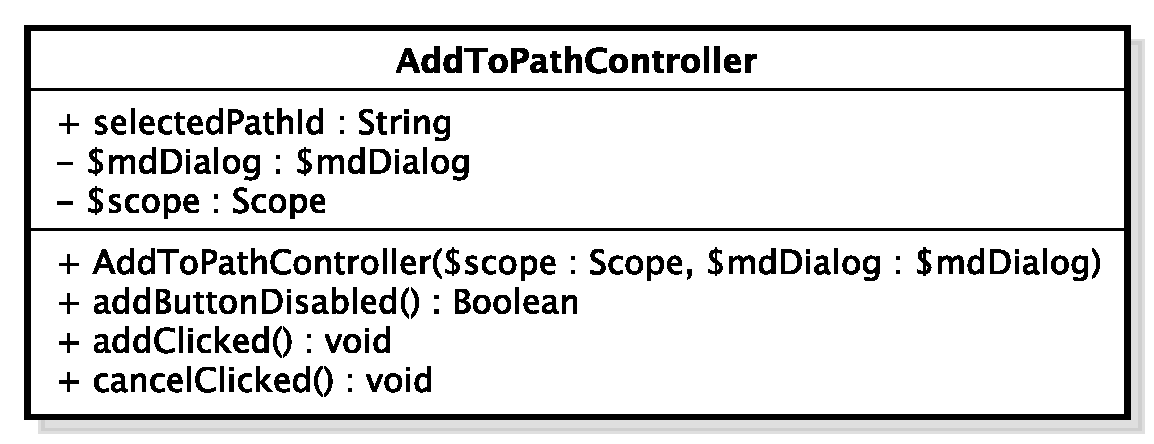
\includegraphics[scale=0.4,keepaspectratio]{diagrammi/classi/{frontEnd/controllers/AddToPathController}.pdf}}
\caption{\nogloxy{Premi::Front-End::Controllers::AddToPathController}}
\end{figure}
\FloatBarrier
\begin{itemize}
\item \textbf{Descrizione}\\
Classe che si occupa di gestire la logica di funzionamento della directive \texttt{premiAddToPath}.
\item \textbf{Utilizzo}\\
Viene utilizzata per permettere all'utente di aggiungere nodi ai \gloxy{percorsi} di presentazione.
\item \textbf{Relazioni con altre classi}:
\begin{itemize}
\item \textit{OUT} \hyperref[\nogloxy{Premi::Front-End::Directives::premiAddToPath}]{\nogloxy{\texttt{premiAddToPath}}}\\
Rappresenta il componente grafico che permette all’utente di visualizzare il contenuto di un nodo e di aggiungerlo ad uno dei \gloxy{percorsi di presentazione} esistenti.
Questo componente visualizza una lista contenente tutti i \gloxy{percorsi} disponibili al quale, selezionando quello desiderato, è possibile aggiungere il nodo slezionato.
\end{itemize}
\item \textbf{Attributi}:
\begin{itemize}
\item \nogloxy{\texttt{+ selectedPathId: String}}
\\ Campo dati contenente l'\texttt{id} del \gloxy{percorso di presentazione} selezionato dall'utente.
\item \nogloxy{\texttt{- \$mdDialog: \$mdDialog}}
\\ \dpMDDialogServiceField
\item \nogloxy{\texttt{- \$scope: Scope}}
\\ \dpScopeField
\end{itemize}
\item \textbf{Metodi}:
\begin{itemize}
\item \nogloxy{\texttt{+ addButtonDisabled(): Boolean}}
\\ Metodo che ritorna un valore booleano che specifica se il pulsante di conferma è abilitato o meno.
\item \nogloxy{\texttt{+ addClicked(): void}}
\\ Metodo che gestisce l'evento \texttt{click} sul pulsante per confermare l'aggiunta del nodo al \gloxy{percorso} di presentazione.
\item \nogloxy{\texttt{+ AddToPathController(\$scope: Scope, \$mdDialog: \$mdDialog)}}
\\ \dpConstructor
\\ \textbf{Parametri}:
\begin{itemize}
\item \nogloxy{\texttt{\$scope: Scope}}
\\ \dpScopeParam
\item \nogloxy{\texttt{\$mdDialog: \$mdDialog}}
\\ \dpMDDialogServiceParam
\end{itemize}
\item \nogloxy{\texttt{+ cancelClicked(): void}}
\\ Metodo che gestisce l'evento \texttt{click} sul pulsante che annulla l'aggiunta del nodo al \gloxy{percorso} di presentazione.
\end{itemize}
\end{itemize}
\subsubsubsection{\nogloxy{Premi::Front-End::Controllers::AssociationAdderController}}
\label{\nogloxy{Premi::Front-End::Controllers::AssociationAdderController}}
\begin{figure}[h]
\centering
\nogloxy{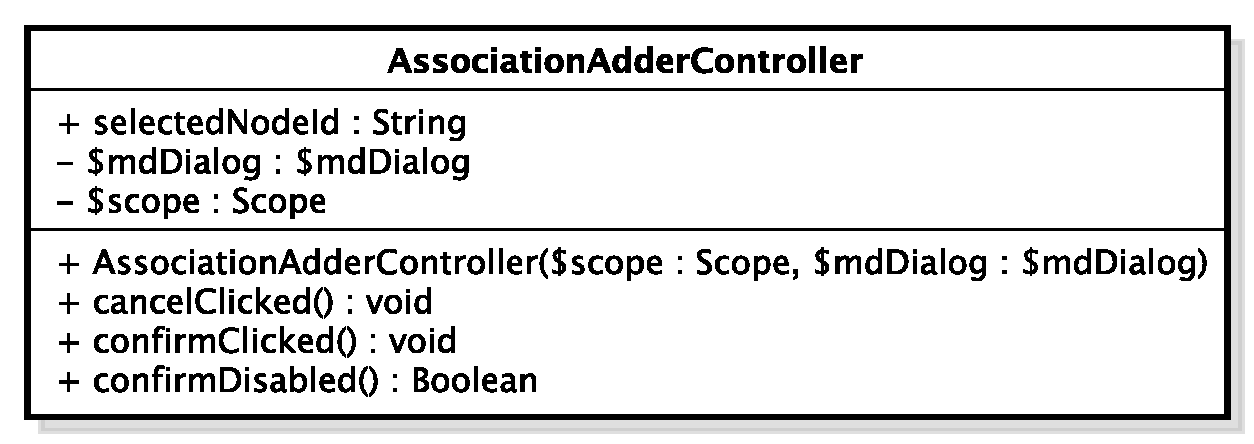
\includegraphics[scale=0.4,keepaspectratio]{diagrammi/classi/{frontEnd/controllers/AssociationAdderController}.pdf}}
\caption{\nogloxy{Premi::Front-End::Controllers::AssociationAdderController}}
\end{figure}
\FloatBarrier
\begin{itemize}
\item \textbf{Descrizione}\\
Classe che gestisce il funzionamento della directive \texttt{premiAssociationAdder}.
\item \textbf{Utilizzo}\\
Viene utilizzata per consentire all'utente di aggiungere associazioni tra i nodi della mappa mentale.
\item \textbf{Relazioni con altre classi}:
\begin{itemize}
\item \textit{OUT} \hyperref[\nogloxy{Premi::Front-End::Directives::premiAssociationAdder}]{\nogloxy{\texttt{premiAssociationAdder}}}\\
Rappresenta il componente grafico che permette all’utente di creare un'associazione tra il nodo selezionato e un altro nodo della mappa.
\end{itemize}
\item \textbf{Attributi}:
\begin{itemize}
\item \nogloxy{\texttt{+ selectedNodeId: String}}
\\ Campo dati contenente l'\texttt{id} dell'oggetto \texttt{NodeReference} selezionato dall'utente.
\item \nogloxy{\texttt{- \$mdDialog: \$mdDialog}}
\\ \dpMDDialogServiceField
\item \nogloxy{\texttt{- \$scope: Scope}}
\\ \dpScopeField
\end{itemize}
\item \textbf{Metodi}:
\begin{itemize}
\item \nogloxy{\texttt{+ AssociationAdderController(\$scope: Scope, \$mdDialog: \$mdDialog)}}
\\ \dpConstructor
\\ \textbf{Parametri}:
\begin{itemize}
\item \nogloxy{\texttt{\$scope: Scope}}
\\ \dpScopeParam
\item \nogloxy{\texttt{\$mdDialog: \$mdDialog}}
\\ \dpMDDialogServiceField
\end{itemize}
\item \nogloxy{\texttt{+ cancelClicked(): void}}
\\ Metodo che gestisce l'evento click sul pulsante per annullare l'aggiunta dell'associazione. Si occupa di nascondere la directive.
\item \nogloxy{\texttt{+ confirmClicked(): void}}
\\ Metodo che gestisce l'evento di click sul pulsante di conferma di aggiunta dell'associazione. Questo metodo invoca la funzione \texttt{\$scope.onNodeSelected} e nasconde la directive.
\item \nogloxy{\texttt{+ confirmDisabled(): Boolean}}
\\ Metodo che ritorna un booleano che specifica se il pulsante di conferma è abilitato o meno.
\end{itemize}
\end{itemize}
\subsubsubsection{\nogloxy{Premi::Front-End::Controllers::ContextMenuController}}
\label{\nogloxy{Premi::Front-End::Controllers::ContextMenuController}}
\begin{figure}[h]
\centering
\nogloxy{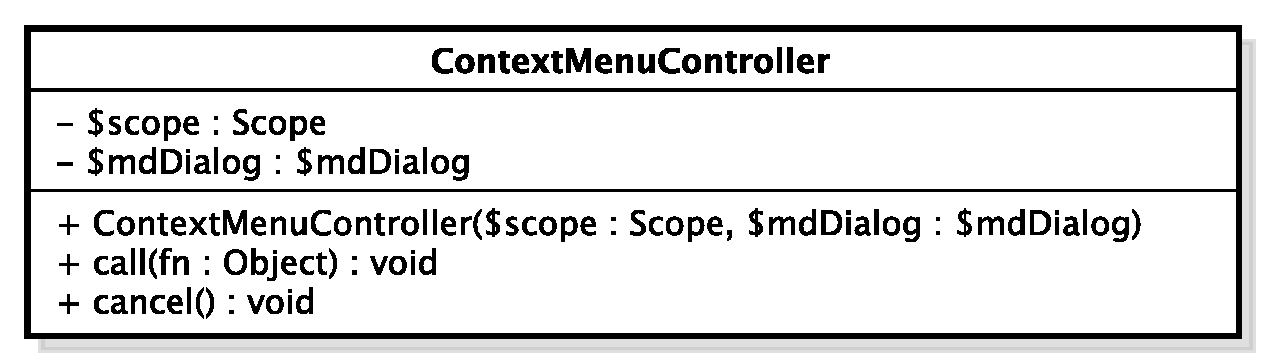
\includegraphics[scale=0.4,keepaspectratio]{diagrammi/classi/{frontEnd/controllers/ContextMenuController}.pdf}}
\caption{\nogloxy{Premi::Front-End::Controllers::ContextMenuController}}
\end{figure}
\FloatBarrier
\begin{itemize}
\item \textbf{Descrizione}\\
Classe che gestisce il comportamento della directive \texttt{premiContextMenu}.
\item \textbf{Utilizzo}\\
Viene utilizzata per gestire il menù che compare quando l'utente seleziona un nodo o un'associazione della mappa mentale.
\item \textbf{Relazioni con altre classi}:
\begin{itemize}
\item \textit{OUT} \hyperref[\nogloxy{Premi::Front-End::Directives::premiContextMenu}]{\nogloxy{\texttt{premiContextMenu}}}\\
Rappresenta un menù contestuale generato in base agli oggetti passati nello scope isolato. Fornisce un pulsante per ogni oggetto ricevuto come parametro, ogni pulsante viene rappresentato con un'icona e con del testo. Al click di un pulsante viene invocata la funzione ad esso associata.
\item \textit{OUT} \hyperref[\nogloxy{Premi::Front-End::Model::Node}]{\nogloxy{\texttt{Node}}}\\
Rappresenta un nodo della mappa mentale. Contiene tutte le informazioni necessarie alla presentazione del contenuto del nodo.
\end{itemize}
\item \textbf{Attributi}:
\begin{itemize}
\item \nogloxy{\texttt{- \$mdDialog: \$mdDialog}}
\\ \dpMDDialogServiceField
\item \nogloxy{\texttt{- \$scope: Scope}}
\\ \dpScopeField
\end{itemize}
\item \textbf{Metodi}:
\begin{itemize}
\item \nogloxy{\texttt{+ call(fn: Object): void}}
\\ Metodo che invoca la funzione la funzione \texttt{\gloxy{callback}} presente all'interno dell'oggetto \texttt{fn} ricevuto come parametro.
\\ \textbf{Parametri}:
\begin{itemize}
\item \nogloxy{\texttt{fn: Object}}
\\ Parametro che rappresenta una voce del menù, ha un campo dati \texttt{\gloxy{callback}} contenente una funzione da invoca quando l'utente seleziona la voce del menù.
\end{itemize}
\item \nogloxy{\texttt{+ cancel(): void}}
\\ Metodo che nasconde il menù utilizzando il metodo \texttt{\$mdDialog.cancel}.
\item \nogloxy{\texttt{+ ContextMenuController(\$scope: Scope, \$mdDialog: \$mdDialog)}}
\\ \dpConstructor
\\ \textbf{Parametri}:
\begin{itemize}
\item \nogloxy{\texttt{\$scope: Scope}}
\\ \dpScopeParam
\item \nogloxy{\texttt{\$mdDialog: \$mdDialog}}
\\ \dpMDDialogServiceParam
\end{itemize}
\end{itemize}
\end{itemize}
\subsubsubsection{\nogloxy{Premi::Front-End::Controllers::DashboardController}}
\label{\nogloxy{Premi::Front-End::Controllers::DashboardController}}
\begin{figure}[h]
\centering
\nogloxy{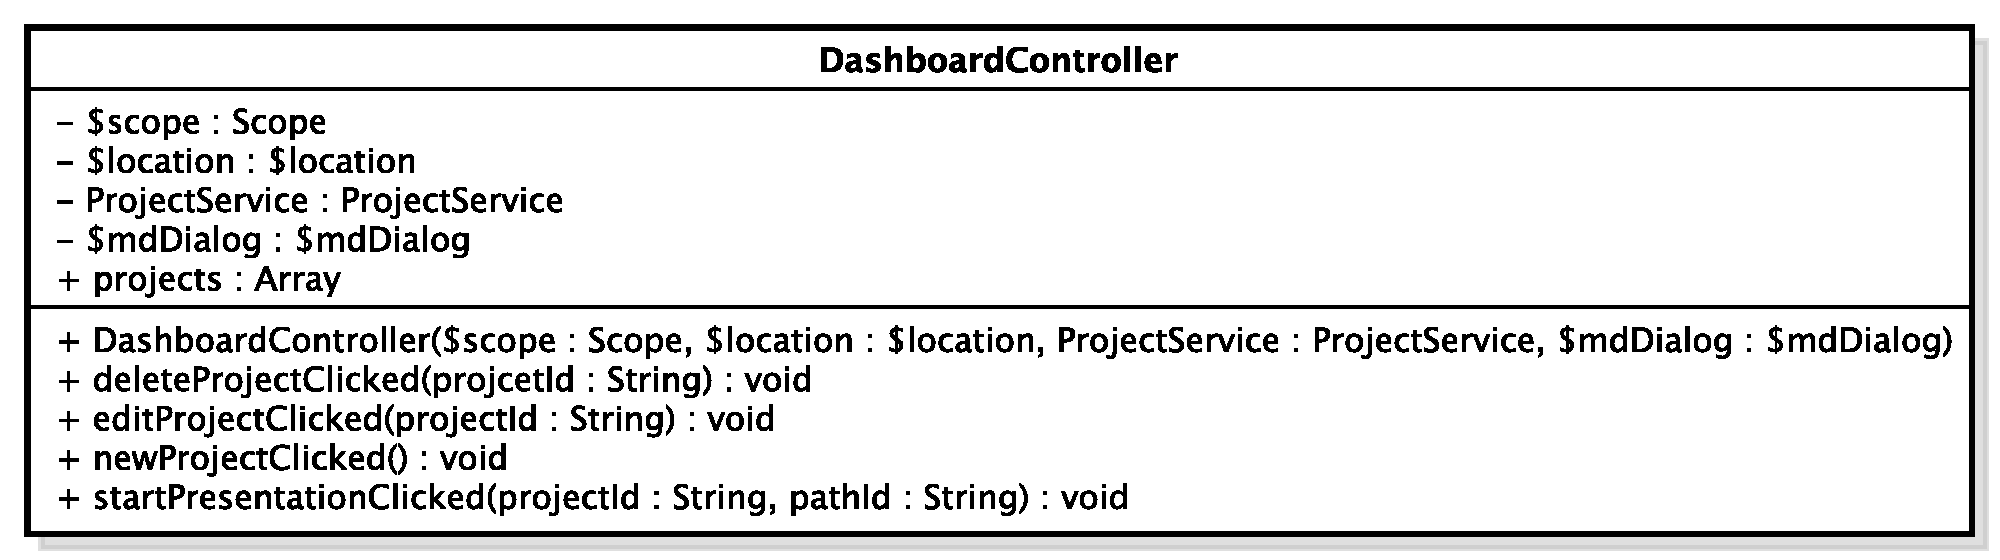
\includegraphics[scale=0.4,keepaspectratio]{diagrammi/classi/{frontEnd/controllers/DashboardController}.pdf}}
\caption{\nogloxy{Premi::Front-End::Controllers::DashboardController}}
\end{figure}
\FloatBarrier
\begin{itemize}
\item \textbf{Descrizione}\\
Classe che gestisce le operazioni e la logica applicativa riguardante la visualizzazione dei \gloxy{progetti} di un utente.
\item \textbf{Utilizzo}\\
Viene utilizzata per consentire all’utente di visualizzare tutti i propri \gloxy{progetti} creati e crearne di nuovi. Dalla lista dei \gloxy{progetti} presenti è possibile selezionare un \gloxy{progetto} per rinominarlo oppure aprirlo, in modo da poterlo modificare e/o presentare.
\item \textbf{Relazioni con altre classi}:
\begin{itemize}
\item \textit{OUT} \hyperref[\nogloxy{Premi::Front-End::Services::ProjectService}]{\nogloxy{\texttt{ProjectService}}}\\
Questa classe si occupa del recupero e della modifica delle informazioni riguardanti i \gloxy{progetti}.
\item \textit{OUT} \hyperref[\nogloxy{Premi::Front-End::Views::DashboardView}]{\nogloxy{\texttt{DashboardView}}}\\
\gloxy{View} dell’applicazione contenente la lista dei \gloxy{progetti} dell’utente correntemente autenticato.
Da questa \gloxy{view} è possibile:
\begin{itemize}
\item Creare un nuovo \gloxy{progetto};
\item Aprire un \gloxy{progetto} esistente per modificarlo oppure presentarlo;
\item Cancellare un \gloxy{progetto} esistente.
\end{itemize}
\end{itemize}
\item \textbf{Attributi}:
\begin{itemize}
\item \nogloxy{\texttt{+ projects: Array}}
\\ Campo dati contenente i \gloxy{progetti} creati dall'utente.
\item \nogloxy{\texttt{- ProjectService: ProjectService}}
\\ Campo dati contenente un riferimento al servizio per la gestione dei \gloxy{progetti}.
\item \nogloxy{\texttt{- \$location: \$location}}
\\ \dpLocationField
\item \nogloxy{\texttt{- \$mdDialog: \$mdDialog}}
\\ \dpMDDialogServiceField
\item \nogloxy{\texttt{- \$scope: Scope}}
\\ \dpScopeField
\end{itemize}
\item \textbf{Metodi}:
\begin{itemize}
\item \nogloxy{\texttt{+ DashboardController(\$scope: Scope, ProjectService: ProjectService, \$location: \$location, \$mdDialog: \$mdDialog)}}
\\ \dpConstructor
\\ \textbf{Parametri}:
\begin{itemize}
\item \nogloxy{\texttt{\$scope: Scope}}
\\ \dpScopeParam
\item \nogloxy{\texttt{ProjectService: ProjectService}}
\\ Parametro che rappresenta il riferimento al servizio di gestione dei \gloxy{progetti}.
\item \nogloxy{\texttt{\$location: \$location}}
\\ \dpLocationParam
\item \nogloxy{\texttt{\$mdDialog: \$mdDialog}}
\\ \dpMDDialogServiceParam
\end{itemize}
\item \nogloxy{\texttt{+ deleteProjectClicked(projectId: String): void}}
\\ Metodo che gestisce l'evento di cancellazione di un \gloxy{progetto} esistente. Interagisce con \texttt{ProjectService} per cancellare il \gloxy{progetto}.
\\ \textbf{Parametri}:
\begin{itemize}
\item \nogloxy{\texttt{projectId: String}}
\\ Parametro contenente l'id del \gloxy{progetto} da cancellare.
\end{itemize}
\item \nogloxy{\texttt{+ editProjectClicked(projectId: String): void}}
\\ Metodo che si occupa di reindirizzare l'utente alla vista per la modifica di un \gloxy{progetto}.
\\ \textbf{Parametri}:
\begin{itemize}
\item \nogloxy{\texttt{projectId: String}}
\\ Parametro contenente l'id del \gloxy{progetto} da aprire.
\end{itemize}
\item \nogloxy{\texttt{+ newProjectClicked(): void}}
\\ Metodo che gestisce l'evento di creazione di un nuovo \gloxy{progetto}. Interagisce con \texttt{ProjectService} per creare un nuovo \gloxy{progetto}.
\item \nogloxy{\texttt{+ startPresentationClicked(pathId: String, projectId: String): void}}
\\ Metodo che gestisce l'avvio di una presentazione direttamente dalla dashboard. Instanzia il \gloxy{progetto} e reindirizza alla vista per la presentazione.
\\ \textbf{Parametri}:
\begin{itemize}
\item \nogloxy{\texttt{pathId: String}}
\\ Parametro contenente l'id del \gloxy{percorso di presentazione} che l'utente vuole presentare.
\item \nogloxy{\texttt{projectId: String}}
\\ Parametro contenente l'id del \gloxy{progetto} contenente il \gloxy{percorso} che l'utente vuole presentare.
\end{itemize}
\end{itemize}
\end{itemize}
\subsubsubsection{\nogloxy{Premi::Front-End::Controllers::EditableNodeContentController}}
\label{\nogloxy{Premi::Front-End::Controllers::EditableNodeContentController}}
\begin{figure}[h]
\centering
\nogloxy{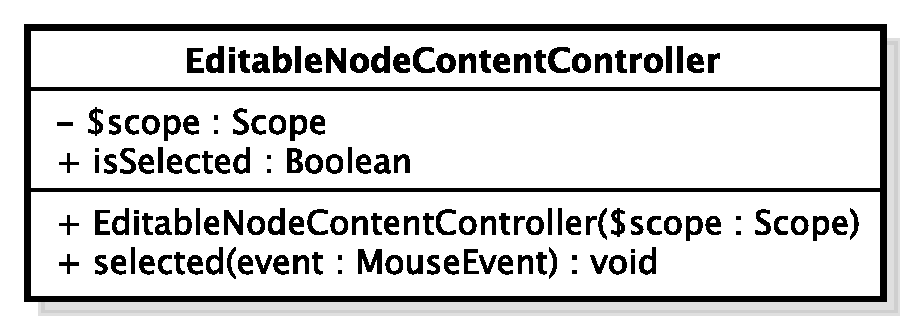
\includegraphics[scale=0.4,keepaspectratio]{diagrammi/classi/{frontEnd/controllers/EditableNodeContentController}.pdf}}
\caption{\nogloxy{Premi::Front-End::Controllers::EditableNodeContentController}}
\end{figure}
\FloatBarrier
\begin{itemize}
\item \textbf{Descrizione}\\
Classe che gestisce la logica della directive \texttt{premiEditableNodeContent}. Questa classe registra un gestore per l'evento \texttt{nodecontent-deselect} che imposta come de-selezionata la directive.
\item \textbf{Utilizzo}\\
Viene utilizzata per gestire la selezione e de-selezione del contenuto di un nodo da parte dell'utente.
\item \textbf{Relazioni con altre classi}:
\begin{itemize}
\item \textit{OUT} \hyperref[\nogloxy{Premi::Front-End::Directives::premiEditableNodeContent}]{\nogloxy{\texttt{premiEditableNodeContent}}}\\
Rappresenta un elemento contenuto nel \gloxy{frame} di un nodo. Questo elemento è spostabile e ridimensionabile. Le modifiche effettuate su questo elemento vengono riportate direttamente sull’oggetto \texttt{nodeContent}.
Questo componente deve essere in grado di rappresentare le varie tipologie di contenuto che possono essere presenti all’interno di un nodo. La discriminazione del tipo del contenuto deve essere fatta in base ai campi dati dell’oggetto \texttt{nodeContent}.
\end{itemize}
\item \textbf{Attributi}:
\begin{itemize}
\item \nogloxy{\texttt{+ isSelected: Boolean}}
\\ Campo dati che specifica se l'elemento è stato selezionato dall'utente o meno.
\item \nogloxy{\texttt{- \$scope: Scope}}
\\ \dpScopeField
\end{itemize}
\item \textbf{Metodi}:
\begin{itemize}
\item \nogloxy{\texttt{+ EditableNodeContentController(\$scope: Scope)}}
\\ \dpConstructor
\\ \textbf{Parametri}:
\begin{itemize}
\item \nogloxy{\texttt{\$scope: Scope}}
\\ \dpScopeParam
\end{itemize}
\item \nogloxy{\texttt{+ selected(event: MouseEvent): void}}
\\ Metodo che gestisce la selezione dell'elemento da parte dell'utente. Questo metodo solleva l'evento \texttt{nodecontent-selected} fornendo l'\texttt{id} dell'oggetto \texttt{NodeContent} rappresentato dalla directive.
\\ \textbf{Parametri}:
\begin{itemize}
\item \nogloxy{\texttt{event: MouseEvent}}
\\ Parametro contenente le informazioni associate all'evento del \gloxy{browser} che ha portato all'invocazione del metodo.
\end{itemize}
\end{itemize}
\end{itemize}
\subsubsubsection{\nogloxy{Premi::Front-End::Controllers::ErrorMessageController}}
\label{\nogloxy{Premi::Front-End::Controllers::ErrorMessageController}}
\begin{figure}[h]
\centering
\nogloxy{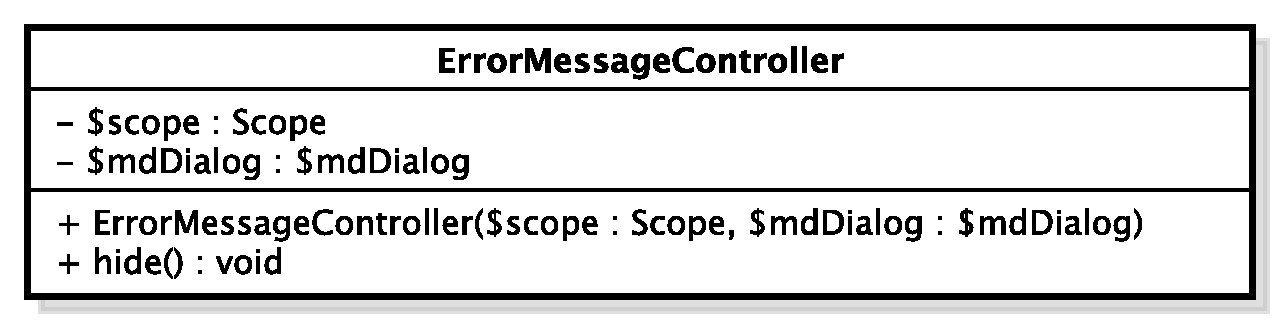
\includegraphics[scale=0.4,keepaspectratio]{diagrammi/classi/{frontEnd/controllers/ErrorMessageController}.pdf}}
\caption{\nogloxy{Premi::Front-End::Controllers::ErrorMessageController}}
\end{figure}
\FloatBarrier
\begin{itemize}
\item \textbf{Descrizione}\\
Classe che gestisce la logica di visualizzazione della directive \texttt{premiErrorMessage}.
\item \textbf{Utilizzo}\\
Viene utilizzata per nascondere la directive quando l'utente prende l'apposito pulsante.
\item \textbf{Relazioni con altre classi}:
\begin{itemize}
\item \textit{OUT} \hyperref[\nogloxy{Premi::Front-End::Directives::premiErrorMessage}]{\nogloxy{\texttt{premiErrorMessage}}}\\
Rappresenta il componente grafico che permette di mostrare messaggi d’errore all’utente all’interno dell’applicazione. Questo componente fornisce anche un pulsante che permette di nascondere il messaggio.
\end{itemize}
\item \textbf{Attributi}:
\begin{itemize}
\item \nogloxy{\texttt{- \$mdDialog: \$mdDialog}}
\\ \dpMDDialogServiceField
\item \nogloxy{\texttt{- \$scope: Scope}}
\\ \dpScopeField
\end{itemize}
\item \textbf{Metodi}:
\begin{itemize}
\item \nogloxy{\texttt{+ ErrorMessageController(\$scope: Scope, \$mdDialog: \$mdDialog)}}
\\ \dpConstructor
\\ \textbf{Parametri}:
\begin{itemize}
\item \nogloxy{\texttt{\$scope: Scope}}
\\ \dpScopeParam
\item \nogloxy{\texttt{\$mdDialog: \$mdDialog}}
\\ \dpMDDialogServiceParam
\end{itemize}
\item \nogloxy{\texttt{+ hide(): void}}
\\ Metodo che nasconde la directive.
\end{itemize}
\end{itemize}
\subsubsubsection{\nogloxy{Premi::Front-End::Controllers::HeaderController}}
\label{\nogloxy{Premi::Front-End::Controllers::HeaderController}}
\begin{figure}[h]
\centering
\nogloxy{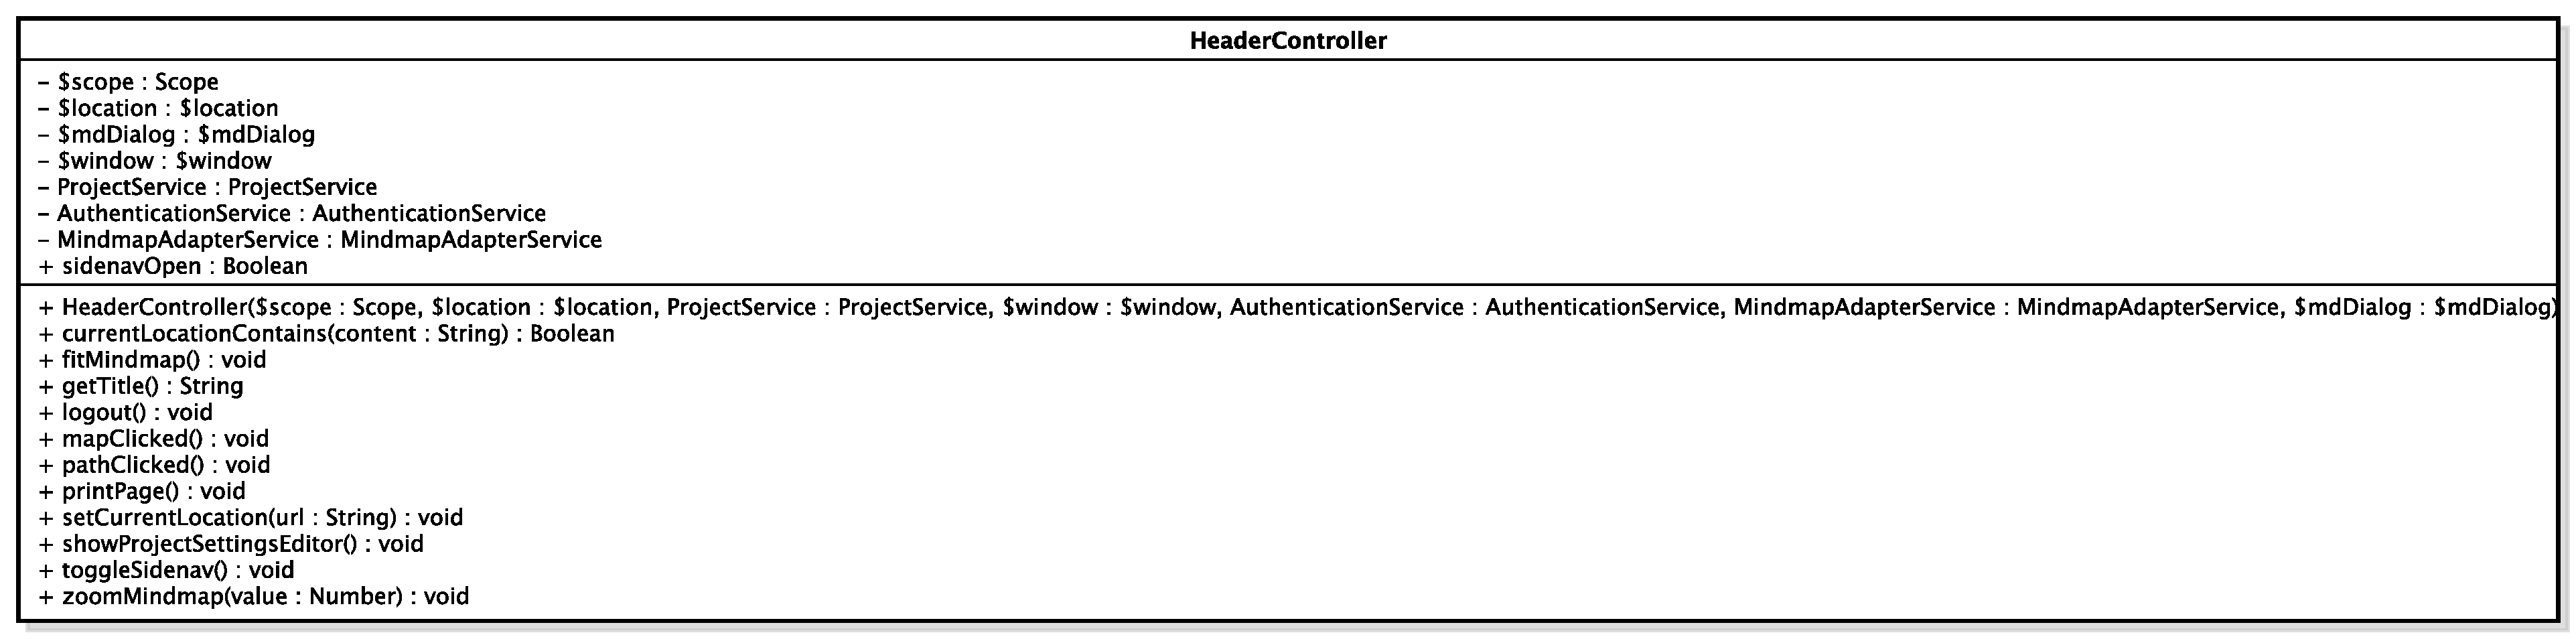
\includegraphics[scale=0.25,keepaspectratio]{diagrammi/classi/{frontEnd/controllers/HeaderController}.pdf}}
\caption{\nogloxy{Premi::Front-End::Controllers::HeaderController}}
\end{figure}
\FloatBarrier
\begin{itemize}
\item \textbf{Descrizione}\\
Classe che gestisce le operazioni e la logica applicativa della directive \texttt{premiHeader},
\item \textbf{Utilizzo}\\
Viene utilizzata per consentire all'utente di spostarsi tra le varie views dell'applicazione.
\item \textbf{Relazioni con altre classi}:
\begin{itemize}
\item \textit{OUT} \hyperref[\nogloxy{Premi::Front-End::Directives::premiHeader}]{\nogloxy{\texttt{premiHeader}}}\\
Rappresenta la barra di navigazione che permette all’utente di spostarsi tra le varie views dell'applicazione. Fornisce inoltre i pulsanti per visualizzare il manuale utente, effettuare il logout, chiudere al presentazione e il \gloxy{progetto}. Inoltre, quando l'utente si trova nelle views in cui è possibile modificare il \gloxy{progetto}, questa directive permette di mostrare la finestra di modifica delle impostazioni del \gloxy{progetto}, sia di interagire con la visualizzazione della mappa mentale, modificando lo zoom e permettendo anche di stamparla.
\end{itemize}
\item \textbf{Attributi}:
\begin{itemize}
\item \nogloxy{\texttt{- AuthenticationService: AuthenticationService}}
\\ \dpAuthenticationServiceField
\item \nogloxy{\texttt{- MindmapAdapterService: MindmapAdapterService}}
\\ \dpMindMapServiceField
\item \nogloxy{\texttt{- ProjectService: ProjectService}}
\\ \dpProjectServiceField
\item \nogloxy{\texttt{+ sidenavOpen: Boolean}}
\\ Campo dati che specifica se il menù laterale è aperto o meno.
\item \nogloxy{\texttt{- \$location: \$location}}
\\ \dpLocationField
\item \nogloxy{\texttt{- \$mdDialog: \$mdDialog}}
\\ \dpMDDialogServiceField
\item \nogloxy{\texttt{- \$scope: Scope}}
\\ \dpScopeField
\item \nogloxy{\texttt{- \$window: \$window}}
\\ \dpWindowServiceField
\end{itemize}
\item \textbf{Metodi}:
\begin{itemize}
\item \nogloxy{\texttt{+ currentLocationContains(content: String): Boolean}}
\\ Metodo che controlla se l'URL corrente contiene la stringa ricevuta come parametro.
\\ \textbf{Parametri}:
\begin{itemize}
\item \nogloxy{\texttt{content: String}}
\\ Parametro che rappresenta il contenuto da cercare.
\end{itemize}
\item \nogloxy{\texttt{+ fitMindmap(): void}}
\\ Metodo che tramite \texttt{MindmapAdapterService} adatta le dimensioni della \gloxy{mappa mentale} a quelle dello schermo.
\item \nogloxy{\texttt{+ getTitle(): String}}
\\ Metodo che, in base alla \gloxy{view} corrente, ritorna il titolo da visualizzare.
\item \nogloxy{\texttt{+ HeaderController(\$scope: Scope, \$location: \$location, ProjectService: ProjectService, \$window: \$window, AuthenticationService: AuthenticationService, MindmapAdapterService: MindmapAdapterService, \$mdDialog: \$mdDialog)}}
\\ \dpConstructor
\\ \textbf{Parametri}:
\begin{itemize}
\item \nogloxy{\texttt{\$scope: Scope}}
\\ \dpScopeParam
\item \nogloxy{\texttt{\$location: \$location}}
\\ \dpLocationParam
\item \nogloxy{\texttt{ProjectService: ProjectService}}
\\ \dpProjectServiceParam
\item \nogloxy{\texttt{\$window: \$window}}
\\ \dpWindowServiceParam
\item \nogloxy{\texttt{AuthenticationService: AuthenticationService}}
\\ \dpAuthenticationServiceParam
\item \nogloxy{\texttt{MindmapAdapterService: MindmapAdapterService}}
\\ \dpMindMapServiceParam
\item \nogloxy{\texttt{\$mdDialog: \$mdDialog}}
\\ \dpMDDialogServiceParam
\end{itemize}
\item \nogloxy{\texttt{+ logout(): void}}
\\ Metodo che gestisce l'evento \texttt{click} sul pulsante per il logout.
\item \nogloxy{\texttt{+ mapClicked(): void}}
\\ Metodo che gestisce l'evento di click sul pulsante per passare alla \gloxy{view} che permette di modificare la mappa mentale, reindirizzando l'utente all'opportuna \gloxy{view}.
\item \nogloxy{\texttt{+ pathClicked(): void}}
\\ Metodo che gestisce l'evento di click sul pulsante per passare alla \gloxy{view} che permette di modificare i \gloxy{percorsi} di presentazione, reindirizzando l'utente all'opportuna \gloxy{view}.
\item \nogloxy{\texttt{+ printPage(): void}}
\\ Metodo che, utilizzando il servizio \texttt{\$window}, invoca la funzionalità di stampa del \gloxy{browser}.
\item \nogloxy{\texttt{+ setCurrentLocation(url: String): void}}
\\ Metodo che reindirizza l'utente alla \gloxy{view} identificata dall'URL ricevuto come parametro.
\\ \textbf{Parametri}:
\begin{itemize}
\item \nogloxy{\texttt{url: String}}
\\ Parametro che rappresenta l'URL da utilizzare per il reindirizzamento.
\end{itemize}
\item \nogloxy{\texttt{+ showManual(ev: MouseEvent): void}}
\\ Metodo che visualizza il pop-up contenente il manuale utente.
\\ \textbf{Parametri}:
\begin{itemize}
\item \nogloxy{\texttt{ev: MouseEvent}}
\\ Parametro contenente le informazioni relative all'evento del \gloxy{browser} che ha portato all'invocazione del metodo.
\end{itemize}
\item \nogloxy{\texttt{+ showProjectSettingsEditor(): void}}
\\ Metodo che utilizzando il servizio \texttt{\$mdDialog} visualizza la directive per la modifica delle impostazioni del \gloxy{progetto} sotto forma di finestra a pop-up.
\item \nogloxy{\texttt{+ toggleSidenav(): void}}
\\ Metodo che inverte il valore del campo dati \texttt{sidenavOpen}.
\item \nogloxy{\texttt{+ zoomMindmap(value: Number): void}}
\\ Metodo che regola lo zoom della mappa mentale, usa \texttt{MindmapAdapterService} per effettuare il ridimensionamento della mappa.
\\ \textbf{Parametri}:
\begin{itemize}
\item \nogloxy{\texttt{value: Number}}
\\ Parametro che rappresenta la quantità di incremento o di decremento dello zoom.
\end{itemize}
\end{itemize}
\end{itemize}
\subsubsubsection{\nogloxy{Premi::Front-End::Controllers::HierarchicalMenuController}}
\label{\nogloxy{Premi::Front-End::Controllers::HierarchicalMenuController}}
\begin{figure}[h]
\centering
\nogloxy{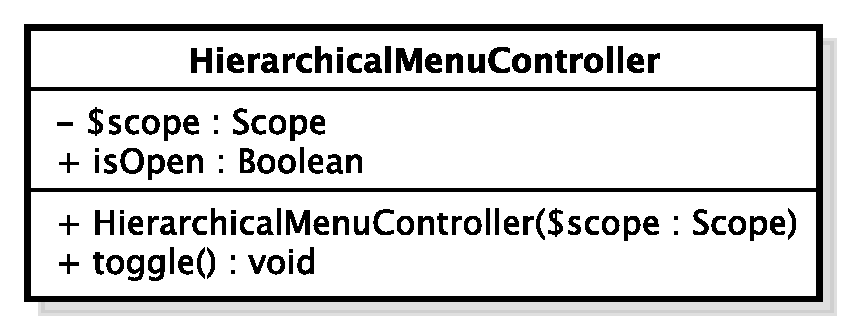
\includegraphics[scale=0.4,keepaspectratio]{diagrammi/classi/{frontEnd/controllers/HierarchicalMenuController}.pdf}}
\caption{\nogloxy{Premi::Front-End::Controllers::HierarchicalMenuController}}
\end{figure}
\FloatBarrier
\begin{itemize}
\item \textbf{Descrizione}\\
Classe che gestisce la visibilità della directive \texttt{premiHierarchicalMenu}.
\item \textbf{Utilizzo}\\
Viene utilizzata per permettere all'utente di nascondere il menù con i nodi in relazione al nodo visualizzato in presentazione.
\item \textbf{Relazioni con altre classi}:
\begin{itemize}
\item \textit{OUT} \hyperref[\nogloxy{Premi::Front-End::Directives::premiHierarchicalMenu}]{\nogloxy{\texttt{premiHierarchicalMenu}}}\\
Rappresenta il menù che durante la presentazione permette di navigare la \gloxy{mappa mentale} seguendo le relazioni gerarchiche presenti tra i vari nodi della mappa mentale. Questo componente consiste in una lista di elementi selezionabili dall’utente, ogni elemento corrisponde ad una relazione presente tra il nodo corrente ed un altro nodo della mappa.
\end{itemize}
\item \textbf{Attributi}:
\begin{itemize}
\item \nogloxy{\texttt{+ isOpen: Boolean}}
\\ Campo dati che specifica se il menù è aperto o chiuso.
\item \nogloxy{\texttt{- \$scope: Scope}}
\\ \dpScopeField
\end{itemize}
\item \textbf{Metodi}:
\begin{itemize}
\item \nogloxy{\texttt{+ HierarchicalMenuController(\$scope: Scope)}}
\\ \dpConstructor
\\ \textbf{Parametri}:
\begin{itemize}
\item \nogloxy{\texttt{\$scope: Scope}}
\\ \dpScopeParam
\end{itemize}
\item \nogloxy{\texttt{+ toggle(): void}}
\\ Metodo che inverte il valore del campo dati \texttt{isOpen}
\end{itemize}
\end{itemize}
\subsubsubsection{\nogloxy{Premi::Front-End::Controllers::LoginController}}
\label{\nogloxy{Premi::Front-End::Controllers::LoginController}}
\begin{figure}[h]
\centering
\nogloxy{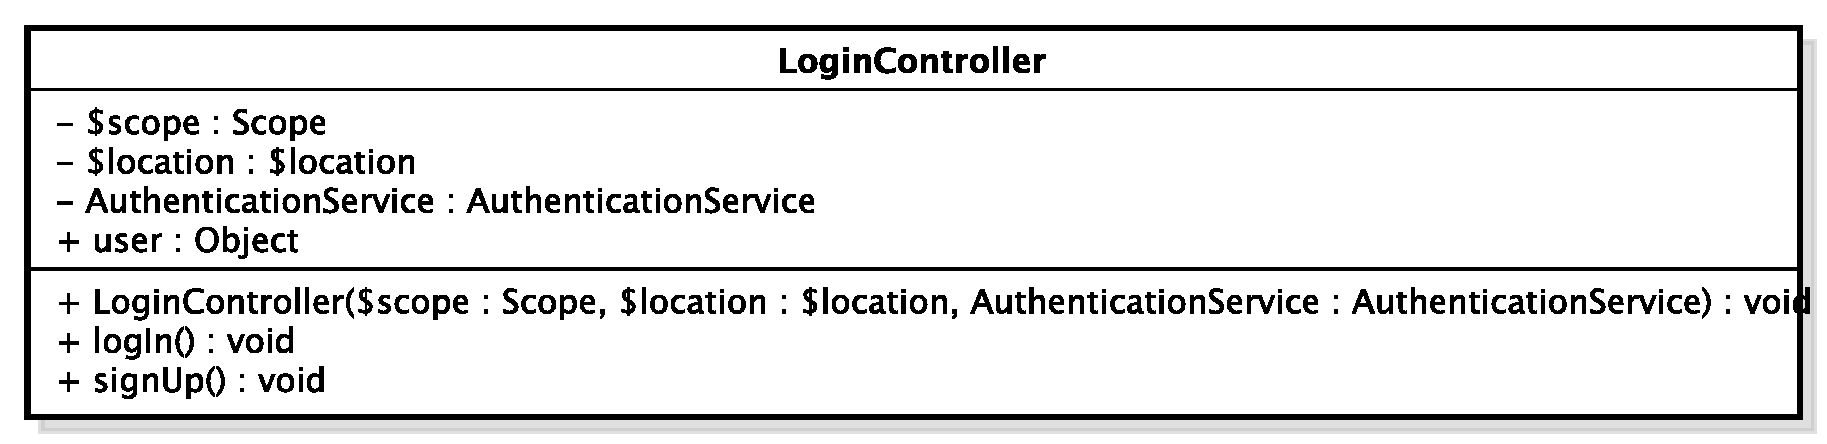
\includegraphics[scale=0.4,keepaspectratio]{diagrammi/classi/{frontEnd/controllers/LoginController}.pdf}}
\caption{\nogloxy{Premi::Front-End::Controllers::LoginController}}
\end{figure}
\FloatBarrier
\begin{itemize}
\item \textbf{Descrizione}\\
Classe che gestisce le operazioni e la logica applicativa riguardante la pagina di login.
\item \textbf{Utilizzo}\\
Viene utilizzata per permettere all’utente di effettuare l’accesso all’applicazione. Prima della creazione della \gloxy{view} viene verificato che non sia già presente una sessione, in caso affermativo l’utente viene reindirizzato alla lista dei \gloxy{progetti} disponibili.
Se non c’è nessuna sessione attiva, viene creata la \gloxy{view} che fornisce all’utente il form necessario per effettuare il login.
Il controllo della sessione e l’autenticazione verranno eseguiti sfruttando \texttt{AuthenticationService}.
\item \textbf{Relazioni con altre classi}:
\begin{itemize}
\item \textit{OUT} \hyperref[\nogloxy{Premi::Front-End::Services::AuthenticationService}]{\nogloxy{\texttt{AuthenticationService}}}\\
Questa classe si occupa di gestire il processo di autenticazione e di registrazione di un utente.
\item \textit{OUT} \hyperref[\nogloxy{Premi::Front-End::Views::LoginView}]{\nogloxy{\texttt{LoginView}}}\\
\gloxy{View} dell’applicazione contenente il form necessario per effettuare il login. Fornisce inoltre un link alla pagina di registrazione.
\end{itemize}
\item \textbf{Attributi}:
\begin{itemize}
\item \nogloxy{\texttt{- AuthenticationService: AuthenticationService}}
\\ \dpAuthenticationServiceField
\item \nogloxy{\texttt{+ user: Object}}
\\ Campo dati contenente un oggetto con i seguenti attributi: \texttt{email} e \texttt{password}.
\item \nogloxy{\texttt{- \$location: \$location}}
\\ \dpLocationField
\item \nogloxy{\texttt{- \$scope: Scope}}
\\ \dpScopeField
\end{itemize}
\item \textbf{Metodi}:
\begin{itemize}
\item \nogloxy{\texttt{+ logIn(): void}}
\\ Metodo che gestisce l'evento click sul pulsante di login. Recupera i dati dallo \$scope e, mediante \texttt{AuthenticationService}, prova ad effettuare l'autenticazione. Se l'autenticazione ha esito positivo, reindirizza l'utente alla dashboard, altrimenti visualizza un messaggio d'errore.
\item \nogloxy{\texttt{+ LoginController(\$scope: Scope, \$location: \$location, AuthenticationService: AuthenticationService)}}
\\ \dpConstructor
\\ \textbf{Parametri}:
\begin{itemize}
\item \nogloxy{\texttt{\$scope: Scope}}
\\ \dpScopeParam
\item \nogloxy{\texttt{\$location: \$location}}
\\ \dpLocationParam
\item \nogloxy{\texttt{AuthenticationService: AuthenticationService}}
\\ \dpAuthenticationServiceParam
\end{itemize}
\item \nogloxy{\texttt{+ signUp(): void}}
\\ Metodo che gestisce l'evento click sul pulsante di registrazione. Effettua il redirect alla pagina di registrazione.
\end{itemize}
\end{itemize}
\subsubsubsection{\nogloxy{Premi::Front-End::Controllers::MindmapEditorController}}
\label{\nogloxy{Premi::Front-End::Controllers::MindmapEditorController}}
\begin{figure}[h]
\centering
\nogloxy{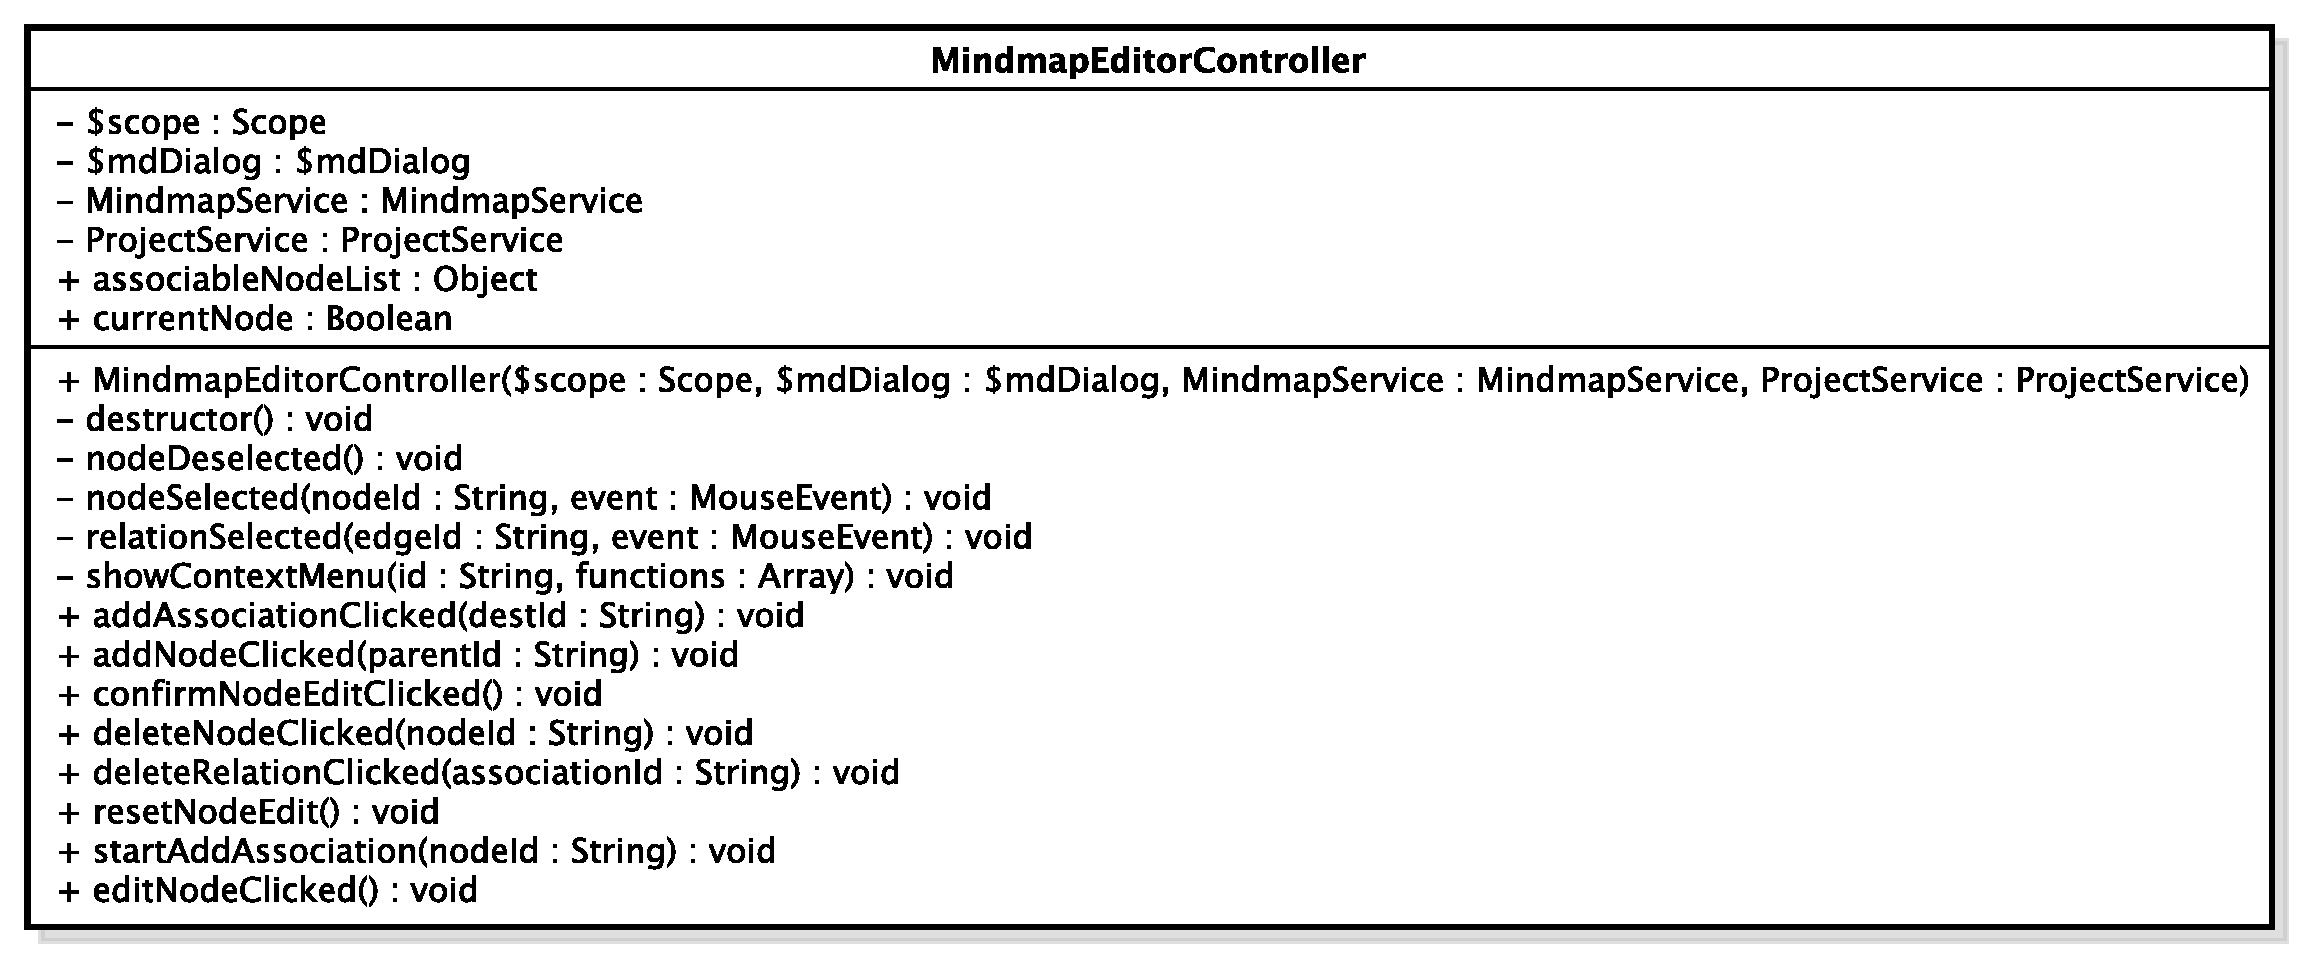
\includegraphics[scale=0.4,keepaspectratio]{diagrammi/classi/{frontEnd/controllers/MindmapEditorController}.pdf}}
\caption{\nogloxy{Premi::Front-End::Controllers::MindmapEditorController}}
\end{figure}
\FloatBarrier
\begin{itemize}
\item \textbf{Descrizione}\\
Classe che gestisce le operazioni e la logica applicativa riguardante la modifica di una mappa.
\item \textbf{Utilizzo}\\
Questa classe viene utilizzata per consentire all’utente di modificare la mappa. In particolare, tramite \texttt{EditMapView} e le directives che la compongono, permette all’utente di:
\begin{itemize}
\item Aggiungere/modificare/eliminare nodi;
\item Aggiungere/eliminare associazioni tra i nodi;
\item Modificare le impostazioni del \gloxy{progetto}.
\end{itemize}
Tutte queste modifiche vengono effettuate utilizzando \texttt{MindmapService}.
\item \textbf{Relazioni con altre classi}:
\begin{itemize}
\item \textit{OUT} \hyperref[\nogloxy{Premi::Front-End::Model::Node}]{\nogloxy{\texttt{Node}}}\\
Rappresenta un nodo della mappa mentale. Contiene tutte le informazioni necessarie alla presentazione del contenuto del nodo.
\item \textit{OUT} \hyperref[\nogloxy{Premi::Front-End::Model::Project}]{\nogloxy{\texttt{Project}}}\\
Rappresenta un \gloxy{progetto} creato dall’utente. Contiene le informazioni riguardanti i parametri globali del \gloxy{progetto}: nome, formato del testo, colore di sfondo.
\item \textit{OUT} \hyperref[\nogloxy{Premi::Front-End::Services::MindmapService}]{\nogloxy{\texttt{MindmapService}}}\\
Questa classe si occupa del recupero e della modifica delle informazioni relative ai nodi e alle associazione presenti nella \gloxy{mappa mentale} del \gloxy{progetto} corrente. Utilizza \texttt{\$http} per comunicare con il \gloxy{back-end} e \texttt{MindmapAdapterService} per memorizzare i dati in locale.
\item \textit{OUT} \hyperref[\nogloxy{Premi::Front-End::Services::ProjectService}]{\nogloxy{\texttt{ProjectService}}}\\
Questa classe si occupa del recupero e della modifica delle informazioni riguardanti i \gloxy{progetti}.
\item \textit{OUT} \hyperref[\nogloxy{Premi::Front-End::Views::MindmapEditorView}]{\nogloxy{\texttt{MindmapEditorView}}}\\
\gloxy{View} dell’applicazione contenente la mappa mentale. Offre funzionalità di modifica della mappa.
Da questa \gloxy{view} è possibile:
\begin{itemize}
\item Aggiungere/togliere nodi;
\item Modificare il contenuto di un nodo;
\item Aggiungere/togliere associazioni tra nodi;
\item Modificare i parametri del \gloxy{progetto}.
\end{itemize}
\end{itemize}
\item \textbf{Attributi}:
\begin{itemize}
\item \nogloxy{\texttt{+ associableNodesList: Object}}
\\ Campo dati contenente le informazioni riguardanti i nodi della \gloxy{mappa mentale} che possono essere associati al \texttt{currentNode}. Le informazioni all'interno dell'oggetto sono memorizzate come coppie chiave/valore, usando come chiave l'\texttt{id} del nodo e come valore il titolo.
\item \nogloxy{\texttt{+ currentNode: Node}}
\\ Campo dati sul quale effettuare le modifiche temporanee prima che l’utente le confermi. Viene usato anche per contenere i dati del nodo da visualizzare in anteprima.
\item \nogloxy{\texttt{- MindmapService: MindmapService}}
\\ \dpNodeServiceField
\item \nogloxy{\texttt{- ProjectService: ProjectService}}
\\ \dpProjectServiceField
\item \nogloxy{\texttt{- \$mdDialog: \$mdDialog}}
\\ \dpMDDialogServiceField
\item \nogloxy{\texttt{- \$scope: Scope}}
\\ \dpScopeField
\end{itemize}
\item \textbf{Metodi}:
\begin{itemize}
\item \nogloxy{\texttt{+ addAssociationClicked(destId: String): void}}
\\ Metodo che gestisce l'evento di creazione di un'associazione tra due nodi. Per creare l'associazione è necessario utilizzare \texttt{AssociationService}, l'informazione riguardante l'origine è disponibile nell'oggetto \texttt{\$scope.currentNode}.
\\ \textbf{Parametri}:
\begin{itemize}
\item \nogloxy{\texttt{destId: String}}
\\ Parametro contenente l'id del nodo destinazione dell'associazione.
\end{itemize}
\item \nogloxy{\texttt{+ addNodeClicked(parentId: String): void}}
\\ Metodo che gestisce l'evento di aggiunta di un nuovo nodo alla mappa mentale. Utilizza \texttt{MindmapService} per aggiungere un nodo vuoto alla mappa mentale, come figlio del nodo passato per parametro.
\\ \textbf{Parametri}:
\begin{itemize}
\item \nogloxy{\texttt{parentId: String}}
\\ Parametro contenente l'id del nodo al quale bisogna aggiungere un nuovo figlio.
\end{itemize}
\item \nogloxy{\texttt{+ confirmNodeEditClicked(): void}}
\\ Metodo che gestisce l'evento di conferma della modifica di un nodo. Rende permanenti le modifiche subite dall'oggetto nodo presente nello \texttt{\$scope}. Utilizza \texttt{MindmpaService}.
\item \nogloxy{\texttt{+ deleteNodeClicked(nodeId: String): void}}
\\ Metodo che gestisce l'evento di cancellazione di un nodo. Utilizza \texttt{MindmapService} per cancellare il nodo dalla mappa mentale.
\\ \textbf{Parametri}:
\begin{itemize}
\item \nogloxy{\texttt{nodeId: String}}
\\ Parametro contenente l'id del nodo da cancellare.
\end{itemize}
\item \nogloxy{\texttt{+ deleteRelationClicked(associationId: String): void}}
\\ Metodo che gestisce l'evento di cancellazione di un'associazione. Utilizza \texttt{MindmapService} per cancellare l'associazione dato l'id.
\\ \textbf{Parametri}:
\begin{itemize}
\item \nogloxy{\texttt{associationId: String}}
\\ Parametro contenente l'id dell'associazione da cancellare.
\end{itemize}
\item \nogloxy{\texttt{- destructor(): void}}
\\ Metodo che gestisce l'evento \texttt{destroy} del \gloxy{controller}, viene utilizzato per interrompere l'ascolto degli eventi di \texttt{MindmapService}.
\item \nogloxy{\texttt{+ editNodeClicked(): void}}
\\ Metodo che gestisce l'evento \texttt{click} sul pulsante che permette di modificare il contenuto del nodo presente nel campo dati \texttt{currentNode}.
\item \nogloxy{\texttt{+ MindmapEditorController(\$scope: Scope, \$mdDialog: \$mdDialog, MindmapService: MindmapService, ProjectService: ProjectService)}}
\\ \dpConstructor
\\ \textbf{Parametri}:
\begin{itemize}
\item \nogloxy{\texttt{\$scope: Scope}}
\\ \dpScopeParam
\item \nogloxy{\texttt{\$mdDialog: \$mdDialog}}
\\ \dpMDDialogServiceParam
\item \nogloxy{\texttt{MindmapService: MindmapService}}
\\ \dpNodeServiceParam
\item \nogloxy{\texttt{ProjectService: ProjectService}}
\\ \dpProjectServiceParam
\end{itemize}
\item \nogloxy{\texttt{- nodeDeselected(): void}}
\\ Metodo che deseleziona il nodo corrente.
\item \nogloxy{\texttt{- nodeSelected(e: MouseEvent, nodeId: String): void}}
\\ Metodo che gestisce l'evento di selezione di un nodo, viene invocato come gestore dell'evento sollevato da \texttt{MindmapService}. Si occupa di aggiornare lo \texttt{\$scope} con i dati del nodo selezionato dall'utente e di visualizzare il menù contestuale in modo da permettere all'utente di modificare il nodo.
\\ \textbf{Parametri}:
\begin{itemize}
\item \nogloxy{\texttt{e: MouseEvent}}
\\ Parametro contenente i dati dell'evento click sollevato dal \gloxy{browser}.
\item \nogloxy{\texttt{nodeId: String}}
\\ Parametro contenente l'id del nodo selezionato dall'utente.
\end{itemize}
\item \nogloxy{\texttt{- relationSelected(e: MouseEvent, edgeId: String): void}}
\\ Metodo che gestisce l'evento di selezione di una relazione, viene invocato come gestore dell'evento sollevato da \texttt{MindmapService}. Si occupa di aggiornare i dati del menù di modifica di una relazione e di visualizzare il menù contestuale per la modifica di un'associazione.
\\ \textbf{Parametri}:
\begin{itemize}
\item \nogloxy{\texttt{e: MouseEvent}}
\\ Parametro contenente i dati dell'evento click sollevato dal \gloxy{browser}.
\item \nogloxy{\texttt{edgeId: String}}
\\ Parametro contenente l'\texttt{id} dell'associazione selezionata dall'utente.
\end{itemize}
\item \nogloxy{\texttt{+ resetNodeEdit(): void}}
\\ Metodo che gestisce l'evento di reset dei campi di modifica di un nodo. Ripristina il \texttt{currentNode} presente nello \texttt{\$scope} utilizzando i dati recuperati da \texttt{MindMapService}.
\item \nogloxy{\texttt{- showContextMenu(id: String, functions: Array): void}}
\\ Metodo che visualizza il menù contestuale.
\\ \textbf{Parametri}:
\begin{itemize}
\item \nogloxy{\texttt{id: String}}
\\ Parametro che rappresenta l'\texttt{id} dell'oggetto sul quale viene visualizzato il menù.
\item \nogloxy{\texttt{functions: Array}}
\\ Parametro che contiene un \texttt{Array} di oggetti rappresentanti le voci del menù. Ogni oggetto ha due campi dati: \texttt{name} e \texttt{\gloxy{callback}}, il primo campo dati specifica il testo associato alla voce del menù e il secondo rappresenta la funzione da chiamare quando l'utente seleziona la voce.
\end{itemize}
\item \nogloxy{\texttt{+ startAddAssociation(sourceId: String): void}}
\\ Metodo che viene invocato quando l'utente seleziona la voce del menù che permette di aggiungere un'associazione uscente dal nodo selezionato.
\\ \textbf{Parametri}:
\begin{itemize}
\item \nogloxy{\texttt{sourceId: String}}
\\ Parametro contenente l'id del nodo sorgente della descrizione.
\end{itemize}
\end{itemize}
\end{itemize}
\subsubsubsection{\nogloxy{Premi::Front-End::Controllers::NodeContentsEditorController}}
\label{\nogloxy{Premi::Front-End::Controllers::NodeContentsEditorController}}
\begin{figure}[h]
\centering
\nogloxy{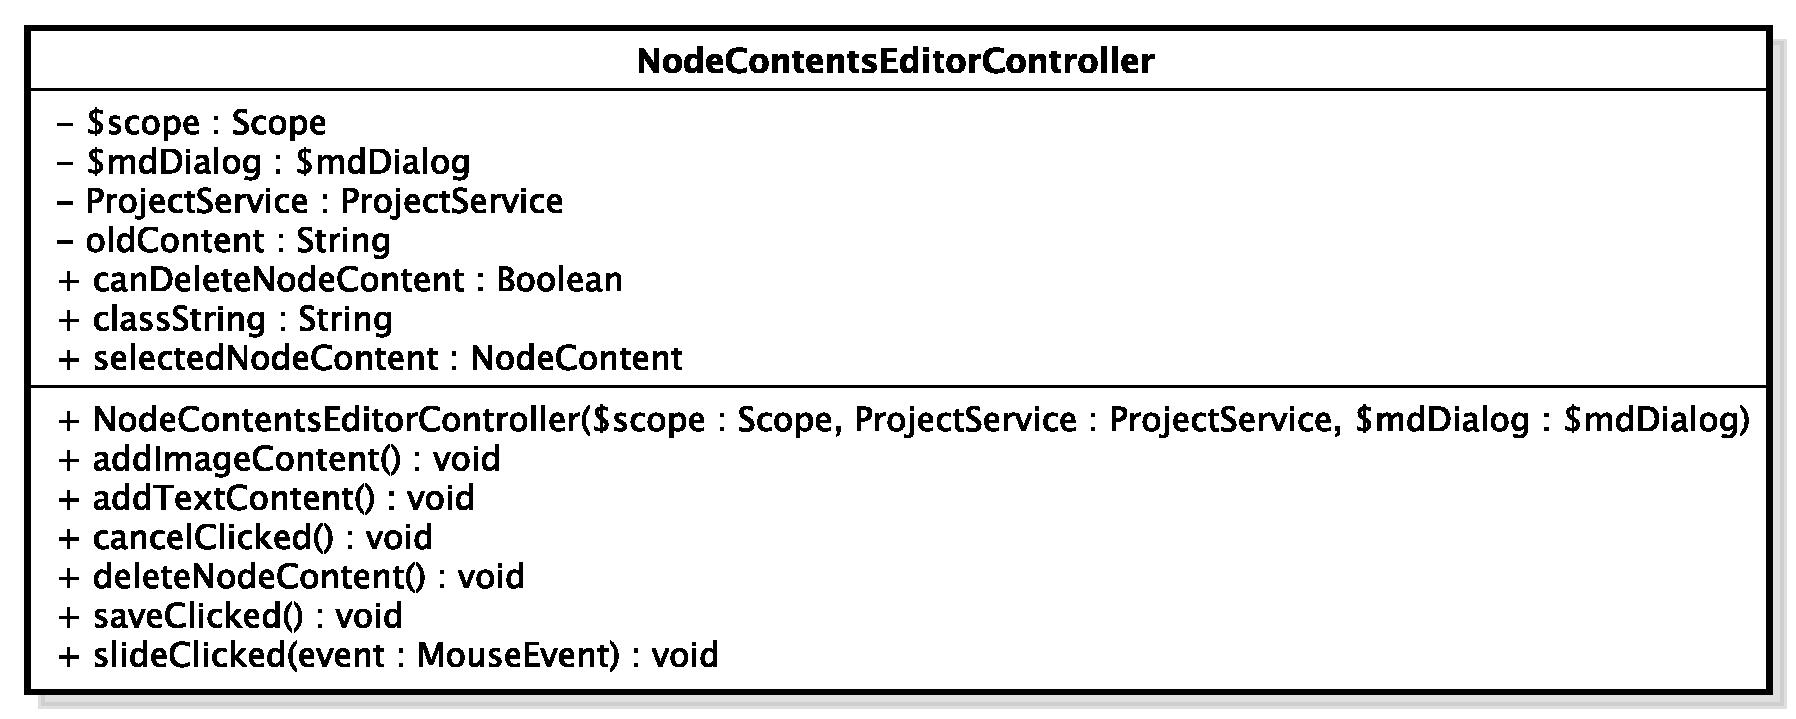
\includegraphics[scale=0.4,keepaspectratio]{diagrammi/classi/{frontEnd/controllers/NodeContentsEditorController}.pdf}}
\caption{\nogloxy{Premi::Front-End::Controllers::NodeContentsEditorController}}
\end{figure}
\FloatBarrier
\begin{itemize}
\item \textbf{Descrizione}\\
Classe che si occupa di gestire la logica legata alla modifica del contenuto di un nodo.
\item \textbf{Utilizzo}\\
Viene utilizzata per consentire all'utente di modificare il contenuto di un nodo.
\item \textbf{Relazioni con altre classi}:
\begin{itemize}
\item \textit{OUT} \hyperref[\nogloxy{Premi::Front-End::Directives::premiNodeContentsEditor}]{\nogloxy{\texttt{premiNodeContentsEditor}}}\\
Rappresenta il componente grafico che permette all’utente di modificare il contenuto di un nodo. Questo componente fornisce all’utente sia dei campi per inserire/modificare il contenuto del nodo, sia un’anteprima di come questo verrà visualizzato. Dall’anteprima sarà anche possibile spostare e ridimensionare i vari componenti.
Saranno presenti inoltre due pulsanti, uno per confermare le modifiche e l’altro per annullarle e ripristinare lo stato del nodo.
\item \textit{OUT} \hyperref[\nogloxy{Premi::Front-End::Model::Node}]{\nogloxy{\texttt{Node}}}\\
Rappresenta un nodo della mappa mentale. Contiene tutte le informazioni necessarie alla presentazione del contenuto del nodo.
\item \textit{OUT} \hyperref[\nogloxy{Premi::Front-End::Model::NodeContent}]{\nogloxy{\texttt{NodeContent}}}\\
Rappresenta il contenuto di un nodo. Contiene informazioni che indicano deve essere visualizzato il contenuto all’interno del nodo.
\item \textit{OUT} \hyperref[\nogloxy{Premi::Front-End::Services::ProjectService}]{\nogloxy{\texttt{ProjectService}}}\\
Questa classe si occupa del recupero e della modifica delle informazioni riguardanti i \gloxy{progetti}.
\end{itemize}
\item \textbf{Attributi}:
\begin{itemize}
\item \nogloxy{\texttt{+ canDeleteNodeContent: Boolean}}
\\ Campo dati che specifica se l'oggetto \texttt{currentNodeContent} può essere cancellato o meno.
\item \nogloxy{\texttt{+ classString: String}}
\\ Campo dati contenente le classi \gloxy{CSS} dello stile del \gloxy{progetto} sotto forma di stringa.
\item \nogloxy{\texttt{- oldContent: String}}
\\ Campo dati che contiene una copia del contenuto dell'oggetto \texttt{NodeContent} che viene selezionato dall'utente. Questo campo dati viene utilizzando per annullare le modifiche dell'utente qualora cercasse di lasciare il contenuto dell'oggetto vuoto.
\item \nogloxy{\texttt{- ProjectService: ProjectService}}
\\ \dpProjectServiceField
\item \nogloxy{\texttt{+ selectedNodeContent: NodeContent}}
\\ Campo dati contenente un riferimento all'oggetto NodeContent selezionato dall'utente.
\item \nogloxy{\texttt{- \$mdDialog: \$mdDialog}}
\\ \dpMDDialogServiceField
\item \nogloxy{\texttt{- \$scope: Scope}}
\\ \dpScopeField
\end{itemize}
\item \textbf{Metodi}:
\begin{itemize}
\item \nogloxy{\texttt{+ addImageContent(): void}}
\\ Metodo che aggiunge all'oggetto \texttt{node} presente nello \texttt{\$scope} un nuovo contenuto di tipo immagine.
\item \nogloxy{\texttt{+ addTextContent(): void}}
\\ Metodo che aggiunge all'oggetto \texttt{node} presente nello \texttt{\$scope} un nuovo contenuto di tipo testuale.
\item \nogloxy{\texttt{+ cancelClicked(): void}}
\\ Metodo che gestisce il click dell'utente sul pulsante per annullare le modifiche. Questo metodo invoca la funzione \texttt{\$scope.onReset} e nasconde la directive.
\item \nogloxy{\texttt{+ deleteNodeContent(): void}}
\\ Metodo che rimuove dall'oggetto \texttt{node} presente nello \texttt{\$scope} l'oggetto \texttt{selectedNodeContent}.
\item \nogloxy{\texttt{+ NodeContentsEditorController(\$scope: Scope, ProjectService: ProjectService, \$mdDialog: \$mdDialog)}}
\\ \dpConstructor
\\ \textbf{Parametri}:
\begin{itemize}
\item \nogloxy{\texttt{\$scope: Scope}}
\\ \dpScopeParam
\item \nogloxy{\texttt{ProjectService: ProjectService}}
\\ \dpProjectServiceParam
\item \nogloxy{\texttt{\$mdDialog: \$mdDialog}}
\\ \dpMDDialogServiceParam
\end{itemize}
\item \nogloxy{\texttt{+ saveClicked(): void}}
\\ Metodo che gestisce il click dell'utente sul pulsante di conferma delle modifiche. Questo metodo invoca la funzione \texttt{\$scope.onConfirm} e nasconde la directive.
\item \nogloxy{\texttt{+ slideClicked(event: MouseEvent): void}}
\\ Metodo che gestisce l'evento \texttt{click} sulla slide, deselezionando l'elemento correntemente selezionato.
\\ \textbf{Parametri}:
\begin{itemize}
\item \nogloxy{\texttt{event: MouseEvent}}
\\ Parametro contenente le informazioni riguardanti l'evento del \gloxy{browser} che ha portato alla chiamata del metodo.
\end{itemize}
\end{itemize}
\end{itemize}
\subsubsubsection{\nogloxy{Premi::Front-End::Controllers::NodeController}}
\label{\nogloxy{Premi::Front-End::Controllers::NodeController}}
\begin{figure}[h]
\centering
\nogloxy{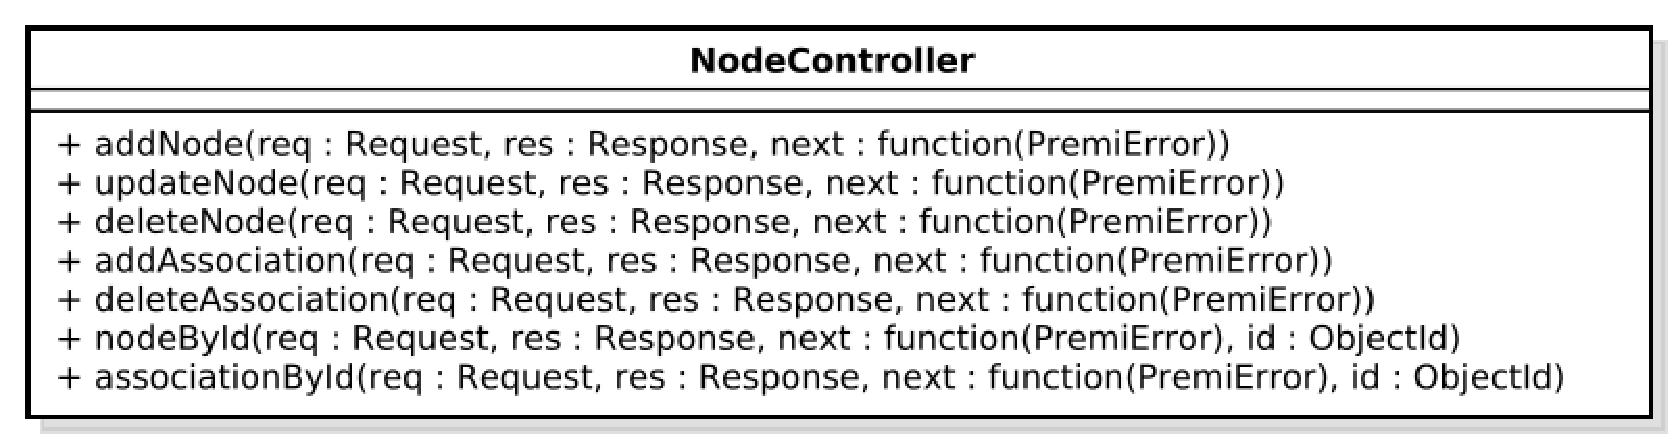
\includegraphics[scale=0.4,keepaspectratio]{diagrammi/classi/{frontEnd/controllers/NodeController}.pdf}}
\caption{\nogloxy{Premi::Front-End::Controllers::NodeController}}
\end{figure}
\FloatBarrier
\begin{itemize}
\item \textbf{Descrizione}\\
Classe che si occupa di gestire il funzionamento della directive \texttt{premiNode}.
\item \textbf{Utilizzo}\\
Viene utilizzata per gestire lo stile di visualizzazione del \gloxy{frame} che deve essere visualizzato dalla directive.
\item \textbf{Relazioni con altre classi}:
\begin{itemize}
\item \textit{OUT} \hyperref[\nogloxy{Premi::Front-End::Directives::premiNode}]{\nogloxy{\texttt{premiNode}}}\\
Rappresenta il componente grafico che visualizza il contenuto di un nodo. Questo contenuto non deve essere modificabile.
\item \textit{OUT} \hyperref[\nogloxy{Premi::Front-End::Model::Node}]{\nogloxy{\texttt{Node}}}\\
Rappresenta un nodo della mappa mentale. Contiene tutte le informazioni necessarie alla presentazione del contenuto del nodo.
\item \textit{OUT} \hyperref[\nogloxy{Premi::Front-End::Services::ProjectService}]{\nogloxy{\texttt{ProjectService}}}\\
Questa classe si occupa del recupero e della modifica delle informazioni riguardanti i \gloxy{progetti}.
\end{itemize}
\item \textbf{Attributi}:
\begin{itemize}
\item \nogloxy{\texttt{+ classString: String}}
\\ Campo dati contenente le classi \gloxy{CSS} che determinano lo stile del \gloxy{progetto}.
\item \nogloxy{\texttt{- ProjectService: ProjectService}}
\\ \dpProjectServiceField
\item \nogloxy{\texttt{- \$scope: Scope}}
\\ \dpScopeField
\end{itemize}
\item \textbf{Metodi}:
\begin{itemize}
\item \nogloxy{\texttt{+ NodeController(\$scope: Scope, ProjectService: ProjectService)}}
\\ \dpConstructor \\ Viene utilizzato per impostare lo stile di visualizzazione del \gloxy{frame}, recuperando le informazioni da \texttt{ProjectService}.
\\ \textbf{Parametri}:
\begin{itemize}
\item \nogloxy{\texttt{\$scope: Scope}}
\\ \dpScopeParam
\item \nogloxy{\texttt{ProjectService: ProjectService}}
\\ \dpProjectServiceParam
\end{itemize}
\end{itemize}
\end{itemize}
\subsubsubsection{\nogloxy{Premi::Front-End::Controllers::PathController}}
\label{\nogloxy{Premi::Front-End::Controllers::PathController}}
\begin{figure}[h]
\centering
\nogloxy{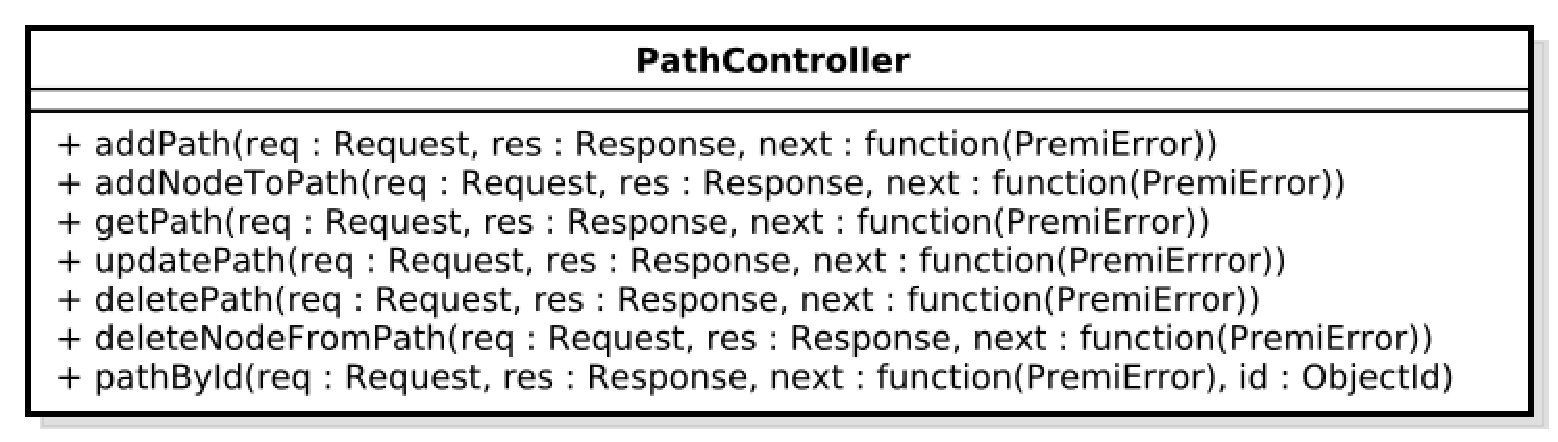
\includegraphics[scale=0.4,keepaspectratio]{diagrammi/classi/{frontEnd/controllers/PathController}.pdf}}
\caption{\nogloxy{Premi::Front-End::Controllers::PathController}}
\end{figure}
\FloatBarrier
\begin{itemize}
\item \textbf{Descrizione}\\
Classe che gestisce la visibilità e la logica della directive \texttt{premiPath}.
\item \textbf{Utilizzo}\\
Viene utilizzata per permettere all'utente di modificare un \gloxy{percorso} di presentazione.
\item \textbf{Relazioni con altre classi}:
\begin{itemize}
\item \textit{OUT} \hyperref[\nogloxy{Premi::Front-End::Directives::premiPath}]{\nogloxy{\texttt{premiPath}}}\\
Rappresenta il componente grafico che permette all’utente di modificare il \gloxy{percorso} selezionato: togliendo dei nodi oppure rinominandolo.
Questo componente visualizza la lista dei nodi presenti nel \gloxy{percorso}. Per ogni nodo viene visualizzato il titolo del nodo ed un pulsante che permette di rimuoverlo dal \gloxy{percorso}.
\item \textit{OUT} \hyperref[\nogloxy{Premi::Front-End::Model::Path}]{\nogloxy{\texttt{Path}}}\\
Rappresenta un \gloxy{percorso di presentazione} costituito da una sequenza ordinata di passi.
\item \textit{OUT} \hyperref[\nogloxy{Premi::Front-End::Services::PathService}]{\nogloxy{\texttt{PathService}}}\\
Questa classe si occupa del recupero e della modifica delle informazioni relative ai \gloxy{percorsi di presentazione} relativi al \gloxy{progetto} corrente.
\end{itemize}
\item \textbf{Attributi}:
\begin{itemize}
\item \nogloxy{\texttt{+ pathName: String}}
\\ Campo dati contenente il nome del \gloxy{percorso} selezionato.
\item \nogloxy{\texttt{- PathService: PathService}}
\\ \dpPathServiceField
\item \nogloxy{\texttt{- \$scope: Scope}}
\\ \dpScopeField
\end{itemize}
\item \textbf{Metodi}:
\begin{itemize}
\item \nogloxy{\texttt{+ PathController(\$scope: Scope, PathService: PathService)}}
\\ \dpConstructor
\\ \textbf{Parametri}:
\begin{itemize}
\item \nogloxy{\texttt{\$scope: Scope}}
\\ \dpScopeParam
\item \nogloxy{\texttt{PathService: PathService}}
\\ \dpPathServiceParam
\end{itemize}
\item \nogloxy{\texttt{+ removeNode(nodeId: String): void}}
\\ Metodo che rimuove il nodo identificato da \texttt{nodeId} dal \gloxy{percorso di presentazione} corrente.
\\ \textbf{Parametri}:
\begin{itemize}
\item \nogloxy{\texttt{nodeId: String}}
\\ Parametro che contiene l'identificativo del nodo da rimuovere dal \gloxy{percorso}.
\end{itemize}
\item \nogloxy{\texttt{+ saveChanges(): void}}
\\ Metodo che rende effettive le modifiche subite dal \gloxy{percorso di presentazione} utilizzando \texttt{PathService}.
\end{itemize}
\end{itemize}
\subsubsubsection{\nogloxy{Premi::Front-End::Controllers::PathsEditorController}}
\label{\nogloxy{Premi::Front-End::Controllers::PathsEditorController}}
\begin{figure}[h]
\centering
\nogloxy{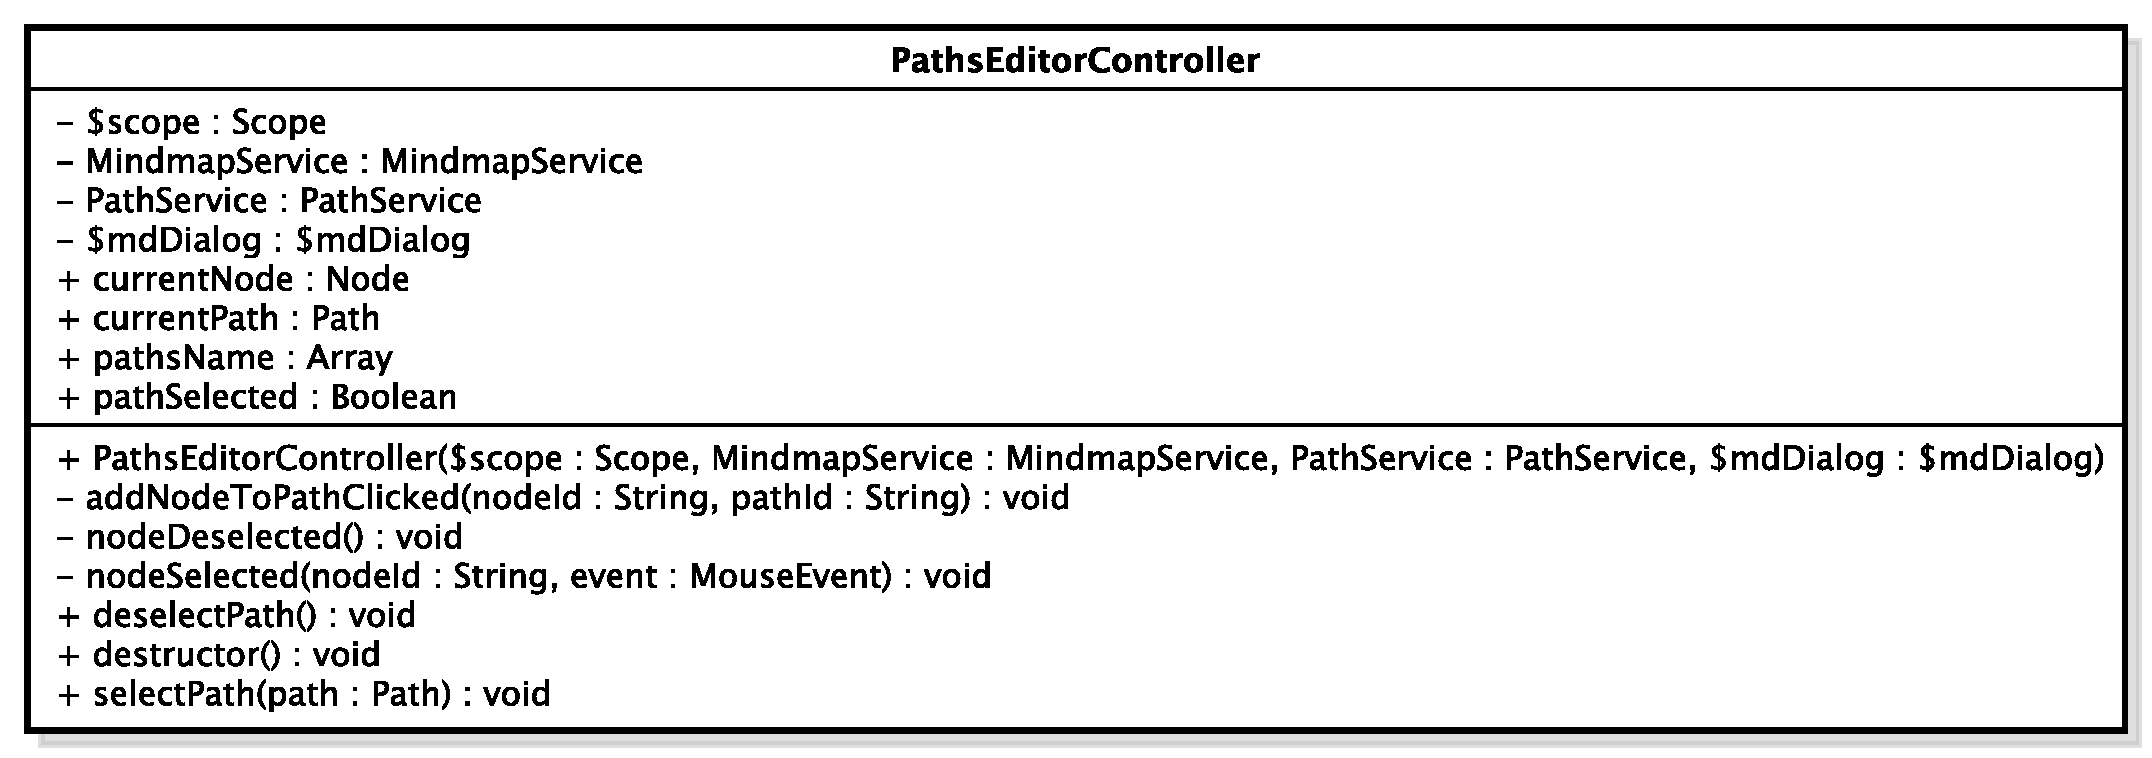
\includegraphics[scale=0.4,keepaspectratio]{diagrammi/classi/{frontEnd/controllers/PathsEditorController}.pdf}}
\caption{\nogloxy{Premi::Front-End::Controllers::PathsEditorController}}
\end{figure}
\FloatBarrier
\begin{itemize}
\item \textbf{Descrizione}\\
Classe che gestisce le operazioni e la logica applicativa riguardante la gestione dei \gloxy{percorsi di presentazione} definiti sulla mappa mentale.
\item \textbf{Utilizzo}\\
Questa classe viene utilizzata per consentire all’utente di creare, modificare e cancellare i \gloxy{percorsi di presentazione} definiti sulla mappa. In particolare, tramite \texttt{PathsEditorView} e le directives che la compongono, permette all’utente di:
\begin{itemize}
\item Creare un nuovo \gloxy{percorso} di presentazione;
\item Modificare un \gloxy{percorso di presentazione} esistente, rinominandolo oppure aggiungendo/togliendo dei nodi al \gloxy{percorso};
\item Eliminare un \gloxy{percorso di presentazione} esistente.
\end{itemize}
Tutte queste modifiche vengono effettuate utilizzando \texttt{PathService}.
Viene fornita anche la possibilità di avviare la presentazione di uno dei \gloxy{percorsi} presenti.
\item \textbf{Relazioni con altre classi}:
\begin{itemize}
\item \textit{OUT} \hyperref[\nogloxy{Premi::Front-End::Model::Node}]{\nogloxy{\texttt{Node}}}\\
Rappresenta un nodo della mappa mentale. Contiene tutte le informazioni necessarie alla presentazione del contenuto del nodo.
\item \textit{OUT} \hyperref[\nogloxy{Premi::Front-End::Model::Path}]{\nogloxy{\texttt{Path}}}\\
Rappresenta un \gloxy{percorso di presentazione} costituito da una sequenza ordinata di passi.
\item \textit{OUT} \hyperref[\nogloxy{Premi::Front-End::Services::MindmapService}]{\nogloxy{\texttt{MindmapService}}}\\
Questa classe si occupa del recupero e della modifica delle informazioni relative ai nodi e alle associazione presenti nella \gloxy{mappa mentale} del \gloxy{progetto} corrente. Utilizza \texttt{\$http} per comunicare con il \gloxy{back-end} e \texttt{MindmapAdapterService} per memorizzare i dati in locale.
\item \textit{OUT} \hyperref[\nogloxy{Premi::Front-End::Services::PathService}]{\nogloxy{\texttt{PathService}}}\\
Questa classe si occupa del recupero e della modifica delle informazioni relative ai \gloxy{percorsi di presentazione} relativi al \gloxy{progetto} corrente.
\item \textit{OUT} \hyperref[\nogloxy{Premi::Front-End::Views::PathsEditorView}]{\nogloxy{\texttt{PathsEditorView}}}\\
\gloxy{View} dell’applicazione contenente la mappa mentale. Offre funzionalità legate ai \gloxy{percorsi} di presentazione.
Da questa \gloxy{view} è possibile:
\begin{itemize}
\item Creare/eliminare un \gloxy{percorso} di presentazione;
\item Modificare un \gloxy{percorso} aggiungendo e togliendo nodi, oppure rinominandolo;
\item Scegliere un \gloxy{percorso} da presentare e successivamente presentarlo.
\end{itemize}
\end{itemize}
\item \textbf{Attributi}:
\begin{itemize}
\item \nogloxy{\texttt{+ currentNode: Node}}
\\ Campo dati contenente le informazioni relative al nodo selezionato dall'utente.
\item \nogloxy{\texttt{+ currentPath: Path}}
\\ Campo dati contenente i dati del \gloxy{percorso} selezionato dall'utente, viene utilizzato per memorizzare le modifiche effettuate dall'utente, ma che non sono ancora state confermate.
\item \nogloxy{\texttt{- MindmapService: MindmapService}}
\\ \dpNodeServiceField
\item \nogloxy{\texttt{+ pathNames: Array}}
\\ Campo dati contenente le informazioni riguardanti i \gloxy{percorsi di presentazione} creati dall'utente. Queste informazioni sono racchiuse in un oggetto con i seguenti attributi: \texttt{$\_$id}, \texttt{name} e \texttt{default}.
\item \nogloxy{\texttt{+ pathSelected: Boolean}}
\\ Campo dati che specifica se l'utente ha selezionato o meno un \gloxy{percorso} di presentazione.
\item \nogloxy{\texttt{- PathService: PathService}}
\\ \dpPathServiceField
\item \nogloxy{\texttt{- \$mdDialog: \$mdDialog}}
\\ \dpMDDialogServiceField
\item \nogloxy{\texttt{- \$scope: Scope}}
\\ \dpScopeField
\end{itemize}
\item \textbf{Metodi}:
\begin{itemize}
\item \nogloxy{\texttt{- addNodeToPathClicked(pathId: String, nodeId: String): void}}
\\ Metodo che gestisce l'evento di aggiunta di un nodo ad un \gloxy{percorso} di presentazione. Aggiunge il nodo identificato da \texttt{nodeId} in coda al \gloxy{percorso} con \texttt{id} uguale a \texttt{pathId}.
\\ \textbf{Parametri}:
\begin{itemize}
\item \nogloxy{\texttt{pathId: String}}
\\ Parametro contenente l'\texttt{id} del \gloxy{percorso di presentazione} al quale aggiungere il nodo.
\item \nogloxy{\texttt{nodeId: String}}
\\ Parametro contenente l'id del nodo da aggiungere al \gloxy{percorso} di presentazione.
\end{itemize}
\item \nogloxy{\texttt{+ deselectPath(): void}}
\\ Metodo che deseleziona il \gloxy{percorso di presentazione} precedentemente selezionato.
\item \nogloxy{\texttt{- destructor(): void}}
\\ Metodo che gestisce l'evento \texttt{destroy} del \gloxy{controller}, viene utilizzato per interrompere l'ascolto degli eventi di \texttt{MindmapService}.
\item \nogloxy{\texttt{- nodeDeselected(): void}}
\\ Metodo che deseleziona il nodo corrente, impostato l'oggetto \texttt{currentNode} a \texttt{null}. Questo metodo viene invocato come gestore dell'evento \texttt{node-delesect} di \texttt{MindmapService}.
\item \nogloxy{\texttt{- nodeSelected(e: MouseEvent, nodeId: String): void}}
\\ Metodo che gestisce l'evento di selezione di un nodo, viene invocato come gestore dell'evento sollevato da \texttt{MindmapService}. Si occupa di aggiornare lo \texttt{\$scope} con i dati del nodo selezionato dall'utente e di rendere visibile la directive per l'aggiunta del nodo selezionato ad un \gloxy{percorso} di presentazione.
\\ \textbf{Parametri}:
\begin{itemize}
\item \nogloxy{\texttt{e: MouseEvent}}
\\ Parametro contenente i dati dell'evento click sollevato dal \gloxy{browser}.
\item \nogloxy{\texttt{nodeId: String}}
\\ Parametro contenente l'id del nodo selezionato.
\end{itemize}
\item \nogloxy{\texttt{+ PathsEditorController(\$scope: Scope, PathService: PathService, MindmapService: MindmapService, \$mdDialog: \$mdDialog)}}
\\ \dpConstructor
\\ \textbf{Parametri}:
\begin{itemize}
\item \nogloxy{\texttt{\$scope: Scope}}
\\ \dpScopeParam
\item \nogloxy{\texttt{PathService: PathService}}
\\ \dpPathServiceParam
\item \nogloxy{\texttt{MindmapService: MindmapService}}
\\ \dpNodeServiceParam
\item \nogloxy{\texttt{\$mdDialog: \$mdDialog}}
\\ \dpMDDialogServiceParam
\end{itemize}
\item \nogloxy{\texttt{+ selectPath(path: Path): void}}
\\ Metodo che imposta il \gloxy{percorso} corrente come riferimento al parametro \texttt{path}.
\\ \textbf{Parametri}:
\begin{itemize}
\item \nogloxy{\texttt{path: Path}}
\\ Parametro che rappresenta il \gloxy{percorso di presentazione} selezionato dall'utente.
\end{itemize}
\end{itemize}
\end{itemize}
\subsubsubsection{\nogloxy{Premi::Front-End::Controllers::PathsListController}}
\label{\nogloxy{Premi::Front-End::Controllers::PathsListController}}
\begin{figure}[h]
\centering
\nogloxy{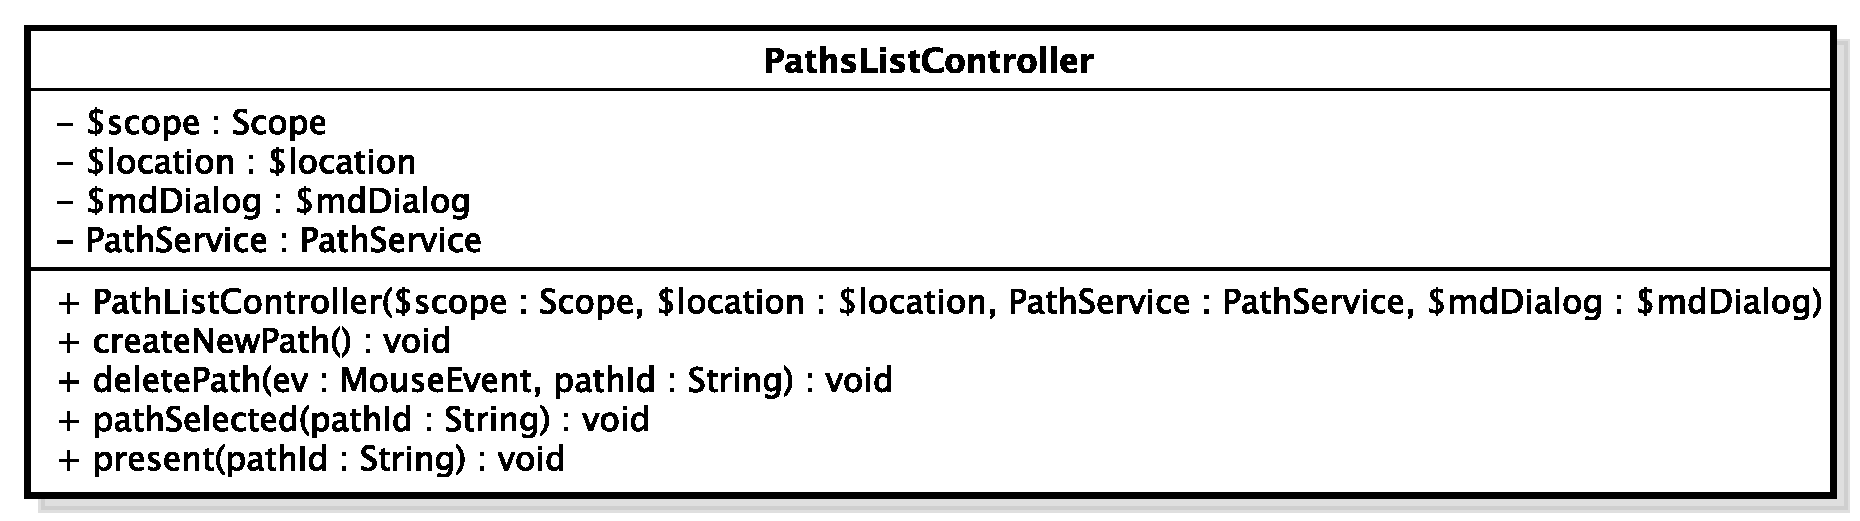
\includegraphics[scale=0.4,keepaspectratio]{diagrammi/classi/{frontEnd/controllers/PathsListController}.pdf}}
\caption{\nogloxy{Premi::Front-End::Controllers::PathsListController}}
\end{figure}
\FloatBarrier
\begin{itemize}
\item \textbf{Descrizione}\\
Classe che gestisce le operazioni e la logica applicativa della directive \texttt{premiPathsList}.
\item \textbf{Utilizzo}\\
Viene utilizzata per permettere all'utente di interagire con la lista dei \gloxy{percorsi di presentazione} presenti nel \gloxy{progetto}.
\item \textbf{Relazioni con altre classi}:
\begin{itemize}
\item \textit{OUT} \hyperref[\nogloxy{Premi::Front-End::Directives::premiPathsList}]{\nogloxy{\texttt{premiPathsList}}}\\
Rappresenta il componente grafico che si occupa di visualizzare la lista dei \gloxy{percorsi di presentazione} presenti nel \gloxy{progetto} corrente. Dalla lista dei \gloxy{percorsi} l'utente può selezionare un \gloxy{percorso} per modificarlo, cancellare un determinato \gloxy{percorso} oppure avviare la presentazione di quel \gloxy{percorso}. Questo componente contiene anche un pulsante per creare un nuovo \gloxy{progetto}.
\item \textit{OUT} \hyperref[\nogloxy{Premi::Front-End::Model::Path}]{\nogloxy{\texttt{Path}}}\\
Rappresenta un \gloxy{percorso di presentazione} costituito da una sequenza ordinata di passi.
\item \textit{OUT} \hyperref[\nogloxy{Premi::Front-End::Services::PathService}]{\nogloxy{\texttt{PathService}}}\\
Questa classe si occupa del recupero e della modifica delle informazioni relative ai \gloxy{percorsi di presentazione} relativi al \gloxy{progetto} corrente.
\end{itemize}
\item \textbf{Attributi}:
\begin{itemize}
\item \nogloxy{\texttt{- PathService: PathService}}
\\ \dpPathServiceField
\item \nogloxy{\texttt{- \$location: \$location}}
\\ \dpLocationField
\item \nogloxy{\texttt{- \$mdDialog: \$mdDialog}}
\\ \dpMDDialogServiceField
\item \nogloxy{\texttt{- \$scope: Scope}}
\\ \dpScopeField
\end{itemize}
\item \textbf{Metodi}:
\begin{itemize}
\item \nogloxy{\texttt{+ createNewPath(): void}}
\\ Metodo che utilizza \texttt{PathService} per creare un nuovo \gloxy{percorso} di presentazione.
\item \nogloxy{\texttt{+ deletePath(ev: MouseEvent, pathId: String): void}}
\\ Metodo che richiede a \texttt{PathService} la rimozione del \gloxy{percorso} identificato da \texttt{pathId}.
\\ \textbf{Parametri}:
\begin{itemize}
\item \nogloxy{\texttt{ev: MouseEvent}}
\\ Parametro che rappresenta l'evento del \gloxy{browser} che ha causato l'invocazione del metodo.
\item \nogloxy{\texttt{pathId: String}}
\\ Parametro che rappresenta l'identificativo del \gloxy{percorso di presentazione} che si vuole cancellare.
\end{itemize}
\item \nogloxy{\texttt{+ pathSelected(pathId: String): void}}
\\ Metodo che gestisce il click dell'utente sul pulsante di modifica del \gloxy{percorso} identificato da \texttt{pathId}. Ottiene da \texttt{PathService} l'oggetto \texttt{Path} rappresentante il \gloxy{percorso di presentazione} selezionato ed invoca la funzione \texttt{selectPath} presente nello \texttt{\$scope}.
\\ \textbf{Parametri}:
\begin{itemize}
\item \nogloxy{\texttt{pathId: String}}
\\ Parametro che rappresenta l'\texttt{id} del \gloxy{percorso} che si vuole selezionare.
\end{itemize}
\item \nogloxy{\texttt{+ PathsListController(\$scope: Scope, \$location: \$location, PathService: PathService, \$mdDialog: \$mdDialog)}}
\\ \dpConstructor
\\ \textbf{Parametri}:
\begin{itemize}
\item \nogloxy{\texttt{\$scope: Scope}}
\\ \dpScopeParam
\item \nogloxy{\texttt{\$location: \$location}}
\\ \dpLocationParam
\item \nogloxy{\texttt{PathService: PathService}}
\\ \dpPathServiceParam
\item \nogloxy{\texttt{\$mdDialog: \$mdDialog}}
\\ \dpMDDialogServiceParam
\end{itemize}
\item \nogloxy{\texttt{+ present(pathId: String): void}}
\\ Metodo che avvia la presentazione del \gloxy{percorso} identificato da \texttt{pathId}.
\\ \textbf{Parametri}:
\begin{itemize}
\item \nogloxy{\texttt{pathId: String}}
\\ Parametro che rappresenta l'\texttt{id} del \gloxy{percorso} che si vuole presentare.
\end{itemize}
\end{itemize}
\end{itemize}
\subsubsubsection{\nogloxy{Premi::Front-End::Controllers::PresentationController}}
\label{\nogloxy{Premi::Front-End::Controllers::PresentationController}}
\begin{figure}[h]
\centering
\nogloxy{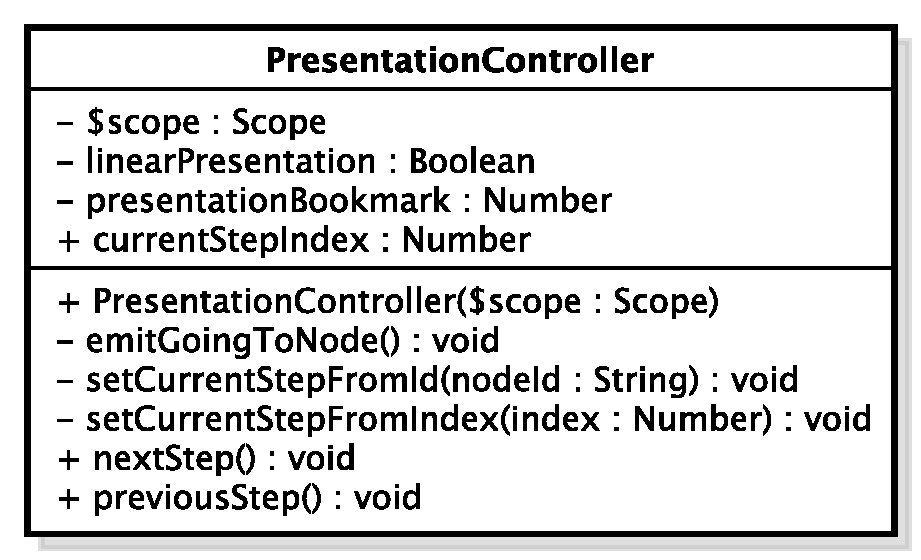
\includegraphics[scale=0.4,keepaspectratio]{diagrammi/classi/{frontEnd/controllers/PresentationController}.pdf}}
\caption{\nogloxy{Premi::Front-End::Controllers::PresentationController}}
\end{figure}
\FloatBarrier
\begin{itemize}
\item \textbf{Descrizione}\\
Classe che si occupa di gestire la logica della presentazione di un \gloxy{percorso}. La gestione della presentazione funziona mediante l'emissione e l'ascolto di determinati eventi.
In particolare questa classe registra dei \textit{listeners} nell'oggetto \texttt{\$scope} per i seguenti eventi:
\begin{itemize}
\item \texttt{presentation-previousStep}: per tornare alla slide precedente;
\item \texttt{presentation-nextStep}: per passare alla slide successiva;
\item \texttt{presentation-goToId}: per passare alla slide contenente il nodo avente \texttt{id} uguale a quello associato all'evento;
\item \texttt{presentation-resumeLinear}: per riprendere la presentazione lineare dopo che si è verificato l'evento \texttt{presentation-goToId}.
\end{itemize}
Viene inoltre sollevato nello \texttt{\$scope} l'evento \texttt{presentation-goingToNode} con l'identificativo del nodo che sta per essere visualizzato ogni volta che si verifica un cambio slide.
\item \textbf{Utilizzo}\\
Viene utilizzata per eseguire la presentazione di un \gloxy{percorso di visualizzazione} definito sulla mappa mentale.
\item \textbf{Relazioni con altre classi}:
\begin{itemize}
\item \textit{OUT} \hyperref[\nogloxy{Premi::Front-End::Directives::premiPresentation}]{\nogloxy{\texttt{premiPresentation}}}\\
Rappresenta il componente grafico che genera la presentazione.
\end{itemize}
\item \textbf{Attributi}:
\begin{itemize}
\item \nogloxy{\texttt{+ currentStepIndex: Number}}
\\ Campo dati che rappresenta l'indice della slide corrente, all'interno della sequenza della presentazione.
\item \nogloxy{\texttt{- linearPresentation: Boolean}}
\\ Campo dati che specifica se la presentazione in corso è lineare o meno, se la presentazione non è lineare i due gestori per gli eventi di passaggio alla slide precedente/successiva sono disattivati.
\item \nogloxy{\texttt{- presentationBookmark: Number}}
\\ Campo dati contenente l'indice dell'ultima slide del \gloxy{percorso di presentazione} visualizzata.
\item \nogloxy{\texttt{- \$scope: Scope}}
\\ \dpScopeField
\end{itemize}
\item \textbf{Metodi}:
\begin{itemize}
\item \nogloxy{\texttt{- emitGoingToNode(): void}}
\\ Metodo d'utilità che solleva l'evento \texttt{presentation-goingToNode} utilizzando i dati del nodo correntemente visualizzato.
\item \nogloxy{\texttt{+ nextStep(): void}}
\\ Metodo che visualizza la slide successiva.
\item \nogloxy{\texttt{+ PresentationController(\$scope: Scope)}}
\\ \dpConstructor
\\ \textbf{Parametri}:
\begin{itemize}
\item \nogloxy{\texttt{\$scope: Scope}}
\\ \dpScopeParam
\end{itemize}
\item \nogloxy{\texttt{+ previousStep(): void}}
\\ Metodo che mostra la slide precedente.
\item \nogloxy{\texttt{- setCurrentStepFromId(nodeId: String): void}}
\\ Metodo che visualizza la slide di contenente il nodo avente \texttt{id} uguale a \texttt{nodeId} presente nella sequenza della presentazione.
\\ \textbf{Parametri}:
\begin{itemize}
\item \nogloxy{\texttt{nodeId: String}}
\\ Parametro che rappresenta l'\texttt{id} del nodo da visualizzare.
\end{itemize}
\item \nogloxy{\texttt{- setCurrentStepFromIndex(index: Number): void}}
\\ Metodo che visualizza la slide di indice \texttt{index} della sequenza del \gloxy{percorso} di presentazione.
\\ \textbf{Parametri}:
\begin{itemize}
\item \nogloxy{\texttt{index: Number}}
\\ Parametro contenente l'indice della slide da visualizzare.
\end{itemize}
\end{itemize}
\end{itemize}
\subsubsubsection{\nogloxy{Premi::Front-End::Controllers::PresentationViewerController}}
\label{\nogloxy{Premi::Front-End::Controllers::PresentationViewerController}}
\begin{figure}[h]
\centering
\nogloxy{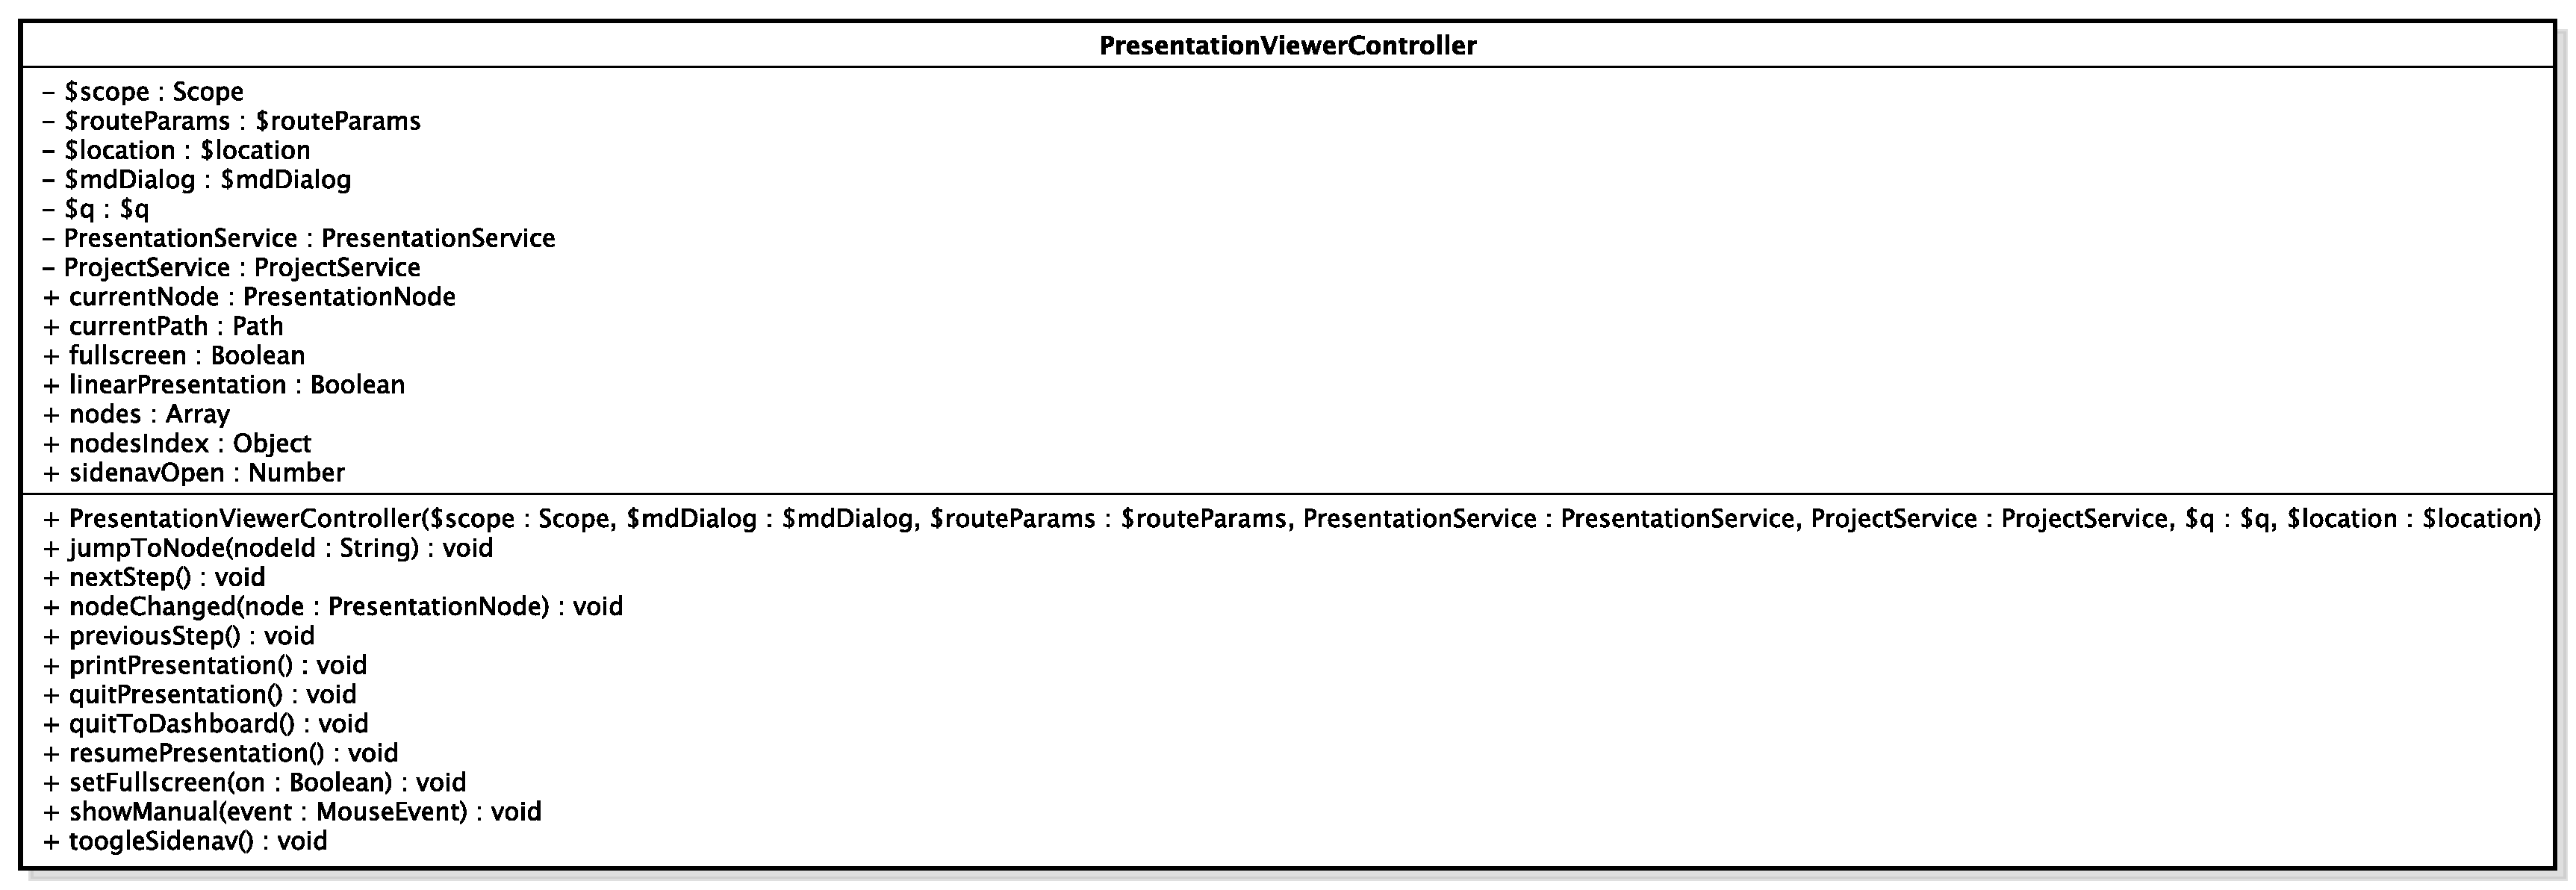
\includegraphics[scale=0.28,keepaspectratio]{diagrammi/classi/{frontEnd/controllers/PresentationViewerController}.pdf}}
\caption{\nogloxy{Premi::Front-End::Controllers::PresentationViewerController}}
\end{figure}
\FloatBarrier
\begin{itemize}
\item \textbf{Descrizione}\\
Classe che gestisce le operazioni e la logica applicativa riguardante l’esecuzione di un \gloxy{percorso} di presentazione.
\item \textbf{Utilizzo}\\
Viene utilizzata per popolare \texttt{PresentationView} con i dati del \gloxy{percorso di presentazione} scelto e per gestire gli eventi legati al cambio di \gloxy{frame}.
\item \textbf{Relazioni con altre classi}:
\begin{itemize}
\item \textit{OUT} \hyperref[\nogloxy{Premi::Front-End::Model::Node}]{\nogloxy{\texttt{Node}}}\\
Rappresenta un nodo della mappa mentale. Contiene tutte le informazioni necessarie alla presentazione del contenuto del nodo.
\item \textit{OUT} \hyperref[\nogloxy{Premi::Front-End::Model::Path}]{\nogloxy{\texttt{Path}}}\\
Rappresenta un \gloxy{percorso di presentazione} costituito da una sequenza ordinata di passi.
\item \textit{OUT} \hyperref[\nogloxy{Premi::Front-End::Model::PresentationNode}]{\nogloxy{\texttt{PresentationNode}}}\\
Classe che estende \texttt{Node}, riproducendo una struttura comoda per poter presentare i contenuti di un nodo e semplificare lo spostamento fra \gloxy{frame} associati e con relazioni di tipo gerarchico.
\item \textit{OUT} \hyperref[\nogloxy{Premi::Front-End::Services::PathService}]{\nogloxy{\texttt{PathService}}}\\
Questa classe si occupa del recupero e della modifica delle informazioni relative ai \gloxy{percorsi di presentazione} relativi al \gloxy{progetto} corrente.
\item \textit{OUT} \hyperref[\nogloxy{Premi::Front-End::Services::PresentationService}]{\nogloxy{\texttt{PresentationService}}}\\
Questa classe si occupa del recupero e della modifica delle informazioni relative alle presentazioni del \gloxy{progetto} corrente.
\item \textit{OUT} \hyperref[\nogloxy{Premi::Front-End::Views::PresentationView}]{\nogloxy{\texttt{PresentationView}}}\\
\gloxy{View} dell’applicazione che permette di effettuare la presentazione di un \gloxy{percorso} scelto dall’utente. Utilizza la directive \texttt{premiPresentation} per offrire funzionalità legate alla presentazione lineare e due menù per permettere all'utente di spostarsi in modo non lineare, seguendo le relazioni definite tra i nodi della mappa mentale.
Da questa vista è inoltre possibile stampare ed esportare il \gloxy{percorso di presentazione} in esecuzione, mediante le funzionalità offerte dal \gloxy{browser}.
\end{itemize}
\item \textbf{Attributi}:
\begin{itemize}
\item \nogloxy{\texttt{+ currentNode: PresentationNode}}
\\ Campo dati contenente le informazioni relative al nodo correntemente visualizzato.
\item \nogloxy{\texttt{+ currentPath: Path}}
\\ Campo dati contenente le informazioni riguardo al \gloxy{percorso di visualizzazione} che viene presentato.
\item \nogloxy{\texttt{+ fullscreen: Boolean}}
\\ Campo dati che specifica se la presentazione in corso è a schermo intero o meno.
\item \nogloxy{\texttt{+ linearPresentation: Boolean}}
\\ Campo dati che specifica se la presentazione in corso è lineare o meno.
\item \nogloxy{\texttt{+ nodes: Array}}
\\ Campo dati contenente una collezione di \texttt{PresentationNode} con tutti i nodi presenti nella mappa mentale, ordinati secondo il \gloxy{percorso di presentazione} scelto dall'utente.
\item \nogloxy{\texttt{+ nodesIndex: Object}}
\\ Campo dati contenente le informazioni riguardante la posizione dei nodi nella sequenza della presentazione. Le informazioni all'interno dell'oggetto sono memorizzate come coppie chiave/valore, usando come chiave l'\texttt{id} del nodo e come valore un \texttt{Array} contenente tutte le posizioni dell'array \texttt{nodes} in cui compare quel determinato nodo.
\item \nogloxy{\texttt{- PresentationService: PresentationService}}
\\ \dpPresentationServiceField
\item \nogloxy{\texttt{- ProjectService: ProjectService}}
\\ \dpProjectServiceField
\item \nogloxy{\texttt{+ sidenavOpen: Boolean}}
\\ Campo dati che specifica se il menù laterale è aperto o meno.
\item \nogloxy{\texttt{- \$location: \$location}}
\\ \dpLocationField
\item \nogloxy{\texttt{- \$mdDialog: \$mdDialog}}
\\ \dpMDDialogServiceField
\item \nogloxy{\texttt{- \$q: \$q}}
\\ \dpQField
\item \nogloxy{\texttt{- \$routeParams: \$routeParams}}
\\ \dpRouteParamsField
\item \nogloxy{\texttt{- \$scope: Scope}}
\\ \dpScopeField
\end{itemize}
\item \textbf{Metodi}:
\begin{itemize}
\item \nogloxy{\texttt{+ jumpToNode(nodeId: String): void}}
\\ Funzione che gestisce il passaggio da un \gloxy{frame} ad un \gloxy{frame} correlato, permettendo di ottenere una presentazione non lineare.
\\ \textbf{Parametri}:
\begin{itemize}
\item \nogloxy{\texttt{nodeId: String}}
\\ Parametro contenente l'id del nodo che sta per essere visualizzato.
\end{itemize}
\item \nogloxy{\texttt{+ nextStep(): void}}
\\ Metodo che fa passare la presentazione alla slide successiva, emettendo l'evento \texttt{presentation-nextStep}
\item \nogloxy{\texttt{+ nodeChanged(node: PresentationNode): void}}
\\ Funzione che gestisce l'evento di passaggio da un \gloxy{frame} all'altro, si occupa di aggiornare le informazioni riguardanti il nodo correntemente visualizzato.
\\ \textbf{Parametri}:
\begin{itemize}
\item \nogloxy{\texttt{node: PresentationNode}}
\\ Parametro contenente il nodo che sta per essere visualizzato.
\end{itemize}
\item \nogloxy{\texttt{+ PresentationViewerController(\$scope: Scope, \$mdSidenav: \$mdSidenav, \$routeParams: \$routeParams, PresentationService: PresentationService, ProjectService: ProjectService)}}
\\ \dpConstructor
\\ \textbf{Parametri}:
\begin{itemize}
\item \nogloxy{\texttt{\$scope: Scope}}
\\ \dpScopeParam
\item \nogloxy{\texttt{\$mdSidenav: \$mdSidenav}}
\\ \dpMDSidenavServiceParam
\item \nogloxy{\texttt{\$routeParams: \$routeParams}}
\\ \dpRouteParamsParam
\item \nogloxy{\texttt{PresentationService: PresentationService}}
\\ \dpPresentationServiceParam
\item \nogloxy{\texttt{ProjectService: ProjectService}}
\\ \dpProjectServiceParam
\end{itemize}
\item \nogloxy{\texttt{+ previousStep(): void}}
\\ Metodo che fa passare la presentazione alla slide precedente, emettendo l'evento \texttt{presentation-previousStep}
\item \nogloxy{\texttt{+ printPresentation(): void}}
\\ Metodo che si occupa di visualizzare la pagina di stampa per la presentazione in corso.
\item \nogloxy{\texttt{+ quitPresentation(): void}}
\\ Metodo che termina la presentazione in corso e che rimanda l'utente alla pagina per la modifica dei \gloxy{percorsi} di presentazione.
\item \nogloxy{\texttt{+ quitToDashboard(): void}}
\\ Metodo che termina la presentazione in corso e che rimanda l'utente alla pagina iniziale.
\item \nogloxy{\texttt{+ resumePresentation(): void}}
\\ Funzione che ripristina la presentazione lineare dopo che l'utente ha navigato ad un \gloxy{frame} fuori dalla presentazione.
\item \nogloxy{\texttt{+ setFullscreen(on: Boolean): void}}
\\ Metodo che permette di entrare oppure uscire dalla modalità a schermo intero, se il parametro ricevuto è \texttt{true} viene attivata la modalità a schermo interno, altrimenti se è \texttt{false} viene disattivata.
\\ \textbf{Parametri}:
\begin{itemize}
\item \nogloxy{\texttt{on: Boolean}}
\\ Parametro che specifica se entrare oppure uscire dalla modalità a schermo intero.
\end{itemize}
\item \nogloxy{\texttt{+ showManual(ev: MouseEvent): void}}
\\ Metodo che visualizza il pop-up contenente il manuale utente.
\\ \textbf{Parametri}:
\begin{itemize}
\item \nogloxy{\texttt{ev: MouseEvent}}
\\ Parametro contenente le informazioni relative all'evento del \gloxy{browser} che ha portato all'invocazione del metodo.
\end{itemize}
\item \nogloxy{\texttt{+ toggleSidenav(): void}}
\\ Metodo che inverte il valore del campo dati \texttt{sidenavOpen}.
\end{itemize}
\end{itemize}
\subsubsubsection{\nogloxy{Premi::Front-End::Controllers::ProjectSettingsEditorController}}
\label{\nogloxy{Premi::Front-End::Controllers::ProjectSettingsEditorController}}
\begin{figure}[h]
\centering
\nogloxy{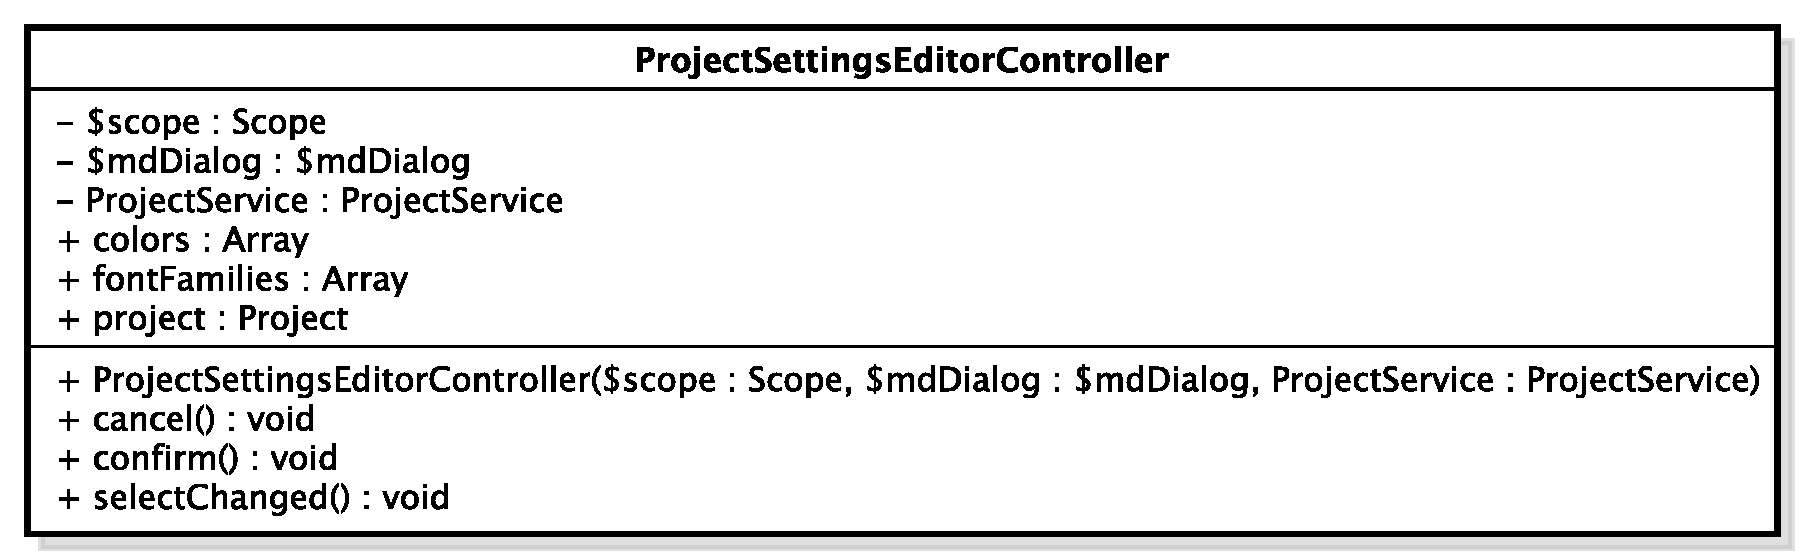
\includegraphics[scale=0.4,keepaspectratio]{diagrammi/classi/{frontEnd/controllers/ProjectSettingsEditorCtrl}.pdf}}
\caption{\nogloxy{Premi::Front-End::Controllers::ProjectSettingsEditorController}}
\end{figure}
\FloatBarrier
\begin{itemize}
\item \textbf{Descrizione}\\
Classe che si occupa di gestire la logica di funzionamento della directive \texttt{premiProjectSettingsEditor}.
\item \textbf{Utilizzo}\\
Viene utilizzata per permettere all'utente di modificare le impostazioni del \gloxy{progetto} aperto.
\item \textbf{Relazioni con altre classi}:
\begin{itemize}
\item \textit{OUT} \hyperref[\nogloxy{Premi::Front-End::Directives::premiProjectSettingsEditor}]{\nogloxy{\texttt{premiProjectSettingsEditor}}}\\
Rappresenta il componente grafico che permette di modificare i dati del \gloxy{progetto} aperto.
Questo componente presenta i vari campi per interagire con i parametri del \gloxy{progetto} e due pulsanti che l'utente utilizza per confermare o annullare le modifiche.
\item \textit{OUT} \hyperref[\nogloxy{Premi::Front-End::Model::Project}]{\nogloxy{\texttt{Project}}}\\
Rappresenta un \gloxy{progetto} creato dall’utente. Contiene le informazioni riguardanti i parametri globali del \gloxy{progetto}: nome, formato del testo, colore di sfondo.
\item \textit{OUT} \hyperref[\nogloxy{Premi::Front-End::Services::ProjectService}]{\nogloxy{\texttt{ProjectService}}}\\
Questa classe si occupa del recupero e della modifica delle informazioni riguardanti i \gloxy{progetti}.
\end{itemize}
\item \textbf{Attributi}:
\begin{itemize}
\item \nogloxy{\texttt{+ colors: Array}}
\\ Campo dati contente una lista di tutti i colori disponibili per il \gloxy{progetto}.
\item \nogloxy{\texttt{+ fontFamilies: Array}}
\\ Campo dati contente una lista di tutti i font disponibili per il \gloxy{progetto}.
\item \nogloxy{\texttt{+ project: Project}}
\\ Campo dati contenente un oggetto che viene utilizzato per memorizzare le modifiche effettuate dall'utente sulle impostazioni del \gloxy{progetto} e che non sono ancora state confermate. L'oggetto ha i seguenti campi dati: \texttt{name}, \texttt{textColor}, \texttt{backgroundColor} e \texttt{fontFamily}.
\item \nogloxy{\texttt{- ProjectService: ProjectService}}
\\ \dpProjectServiceField
\item \nogloxy{\texttt{- \$mdDialog: \$mdDialog}}
\\ \dpMDDialogServiceField
\item \nogloxy{\texttt{- \$scope: Scope}}
\\ \dpScopeField
\end{itemize}
\item \textbf{Metodi}:
\begin{itemize}
\item \nogloxy{\texttt{+ cancel(): void}}
\\ Metodo che gestisce l'evento di click sul pulsante che nasconde la directive.
\item \nogloxy{\texttt{+ confirm(): void}}
\\ Metodo che viene invocato quando l'utente conferma le modifiche al \gloxy{progetto}, si occupa di salvare le modifiche utilizzando \texttt{ProjectService}.
\item \nogloxy{\texttt{+ ProjectSettingsEditorController(\$scope: Scope, \$mdDialog: \$mdDialog, ProjectService: ProjectService)}}
\\ \dpConstructor
\\ \textbf{Parametri}:
\begin{itemize}
\item \nogloxy{\texttt{\$scope: Scope}}
\\ \dpScopeParam
\item \nogloxy{\texttt{\$mdDialog: \$mdDialog}}
\\ \dpMDDialogServiceParam
\item \nogloxy{\texttt{ProjectService: ProjectService}}
\\ \dpProjectServiceParam
\end{itemize}
\item \nogloxy{\texttt{+ selectChanged(): void}}
\\ Metodo che aggiorna l'anteprima dello stile del \gloxy{progetto}, viene invocato ogni volta che l'utente seleziona una nuova opzione per lo stile del \gloxy{progetto}.
\end{itemize}
\end{itemize}
\subsubsubsection{\nogloxy{Premi::Front-End::Controllers::ProjectsListController}}
\label{\nogloxy{Premi::Front-End::Controllers::ProjectsListController}}
\begin{figure}[h]
\centering
\nogloxy{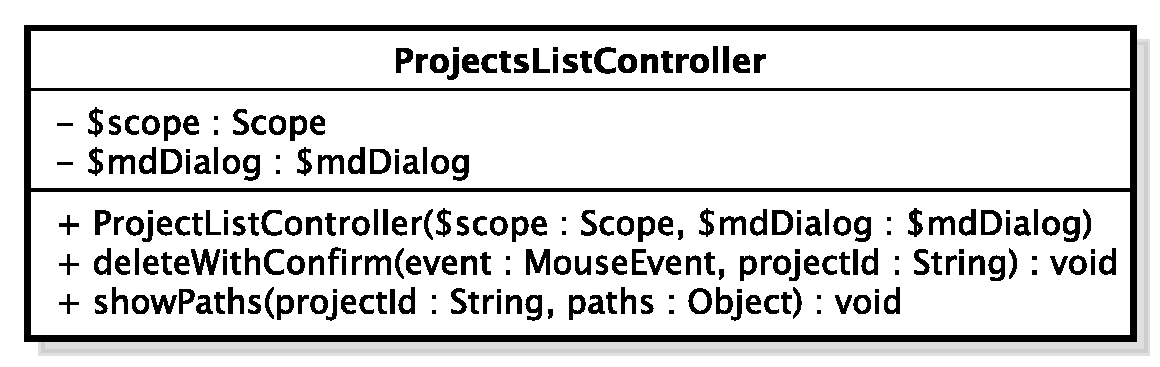
\includegraphics[scale=0.4,keepaspectratio]{diagrammi/classi/{frontEnd/controllers/ProjectsListController}.pdf}}
\caption{\nogloxy{Premi::Front-End::Controllers::ProjectsListController}}
\end{figure}
\FloatBarrier
\begin{itemize}
\item \textbf{Descrizione}\\
Classe che gestisce la logica di funzionamento della directive \texttt{premiProjectsList}.
\item \textbf{Utilizzo}\\
Viene utilizzata per gestire il popup della directive che permette di scegliere un \gloxy{percorso} da presentare.
\item \textbf{Relazioni con altre classi}:
\begin{itemize}
\item \textit{OUT} \hyperref[\nogloxy{Premi::Front-End::Directives::premiProjectsList}]{\nogloxy{\texttt{premiProjectsList}}}\\
Rappresenta il componente grafico che mostra la lista dei \gloxy{progetti} creati dall’utente. Per ogni \gloxy{progetto} della lista è presente un pulsante che permette di modificarlo, di cancellarlo e di presentarlo.
\end{itemize}
\item \textbf{Attributi}:
\begin{itemize}
\item \nogloxy{\texttt{- \$mdDialog: \$mdDialog}}
\\ \dpMDDialogServiceField
\item \nogloxy{\texttt{- \$scope: Scope}}
\\ \dpScopeField
\end{itemize}
\item \textbf{Metodi}:
\begin{itemize}
\item \nogloxy{\texttt{+ deleteWithConfirm(event: MouseEvent, projectId: String): void}}
\\ Metodo che gestisce la cancellazione di un \gloxy{progetto} dalla lista dei \gloxy{progetti}. Prima di effettuare la cancellazione richiede all'utente la conferma dell'operazione.
\\ \textbf{Parametri}:
\begin{itemize}
\item \nogloxy{\texttt{event: MouseEvent}}
\\ Parametro che rappresenta l'evento del \gloxy{browser} che ha causato l'invocazione del metodo.
\item \nogloxy{\texttt{projectId: String}}
\\ Parametro che rappresenta l'\texttt{id} del \gloxy{progetto} da cancellare.
\end{itemize}
\item \nogloxy{\texttt{+ ProjectsListController(\$scope: Scope, \$mdDialog: \$mdDialog)}}
\\ \dpConstructor
\\ \textbf{Parametri}:
\begin{itemize}
\item \nogloxy{\texttt{\$scope: Scope}}
\\ \dpScopeParam
\item \nogloxy{\texttt{\$mdDialog: \$mdDialog}}
\\ \dpMDDialogServiceParam
\end{itemize}
\item \nogloxy{\texttt{+ showPaths(projectId: String, paths: Object): void}}
\\ Metodo che rende visibile la finestra di dialogo per la scelta del \gloxy{percorso di presentazione} da presentare.
\\ \textbf{Parametri}:
\begin{itemize}
\item \nogloxy{\texttt{projectId: String}}
\\ Parametro rappresentate l'\texttt{id} del \gloxy{progetto} contenente il \gloxy{percorso} da presentare.
\item \nogloxy{\texttt{paths: Object}}
\\ Parametro rappresentante i \gloxy{percorsi} disponibili, contiene le informazioni sotto forma di coppie chiave/valore, come chiave viene utilizzato l'\texttt{id} e come valore il nome.
\end{itemize}
\end{itemize}
\end{itemize}
\subsubsubsection{\nogloxy{Premi::Front-End::Controllers::RegistrationController}}
\label{\nogloxy{Premi::Front-End::Controllers::RegistrationController}}
\begin{figure}[h]
\centering
\nogloxy{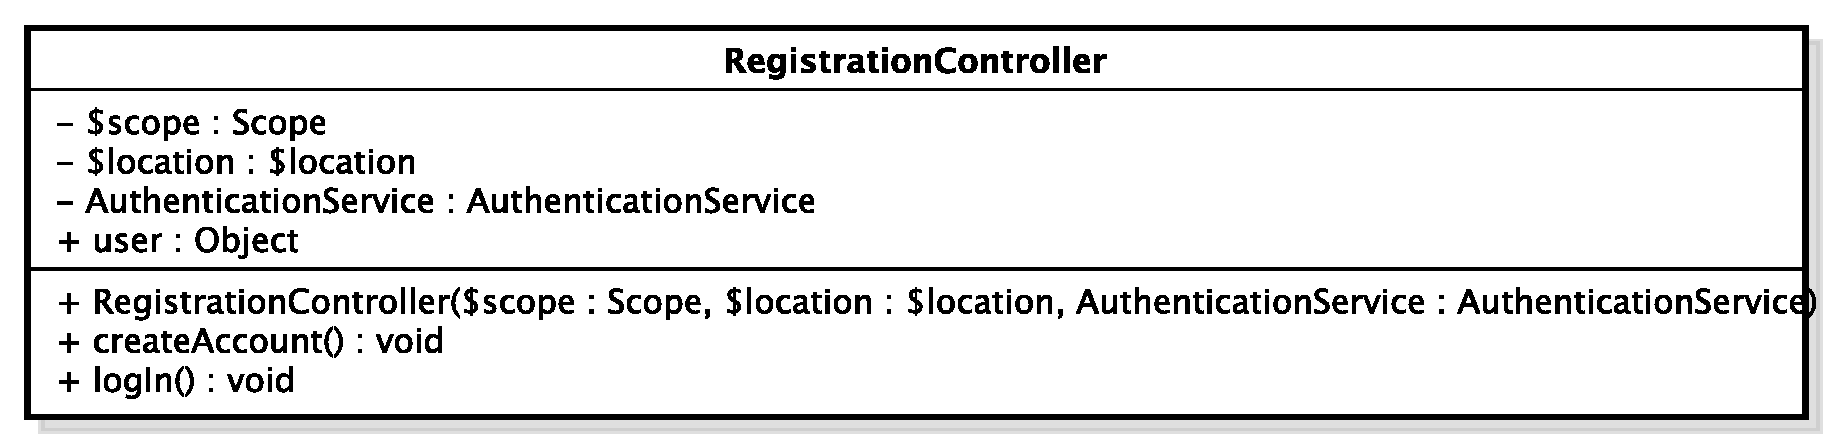
\includegraphics[scale=0.4,keepaspectratio]{diagrammi/classi/{frontEnd/controllers/RegistrationController}.pdf}}
\caption{\nogloxy{Premi::Front-End::Controllers::RegistrationController}}
\end{figure}
\FloatBarrier
\begin{itemize}
\item \textbf{Descrizione}\\
Classe che gestisce le operazioni e la logica applicativa riguardante la registrazione di un utente.
\item \textbf{Utilizzo}\\
Viene utilizzata per gestire la \gloxy{view} di registrazione e per registrare un account sul \gloxy{server}, sfruttando \texttt{AuthenticationService}.
Prima di proporre all’utente la \gloxy{view} di registrazione controlla che non ci sia una sessione già attiva, in tal caso reindirizza l’utente alla lista dei \gloxy{progetti} disponibili.
\item \textbf{Relazioni con altre classi}:
\begin{itemize}
\item \textit{OUT} \hyperref[\nogloxy{Premi::Front-End::Services::AuthenticationService}]{\nogloxy{\texttt{AuthenticationService}}}\\
Questa classe si occupa di gestire il processo di autenticazione e di registrazione di un utente.
\item \textit{OUT} \hyperref[\nogloxy{Premi::Front-End::Views::RegistrationView}]{\nogloxy{\texttt{RegistrationView}}}\\
\gloxy{View} dell’applicazione contenente il form per la registrazione di un nuovo utente. Contiene un link alla pagina di autenticazione.
\end{itemize}
\item \textbf{Attributi}:
\begin{itemize}
\item \nogloxy{\texttt{- AuthenticationService: AuthenticationService}}
\\ \dpAuthenticationServiceField
\item \nogloxy{\texttt{+ user: Object}}
\\ Campo dati contenente un oggetto con i seguenti attributi: \texttt{email}, \texttt{password} e \texttt{passwordCheck}.
\item \nogloxy{\texttt{- \$location: \$location}}
\\ \dpLocationField
\item \nogloxy{\texttt{- \$scope: Scope}}
\\ \dpScopeField
\end{itemize}
\item \textbf{Metodi}:
\begin{itemize}
\item \nogloxy{\texttt{+ createAccount(): void}}
\\ Metodo che gestisce l'evento di pressione del pulsante per la registrazione. Legge dallo \texttt{\$scope} i valori inseriti dall'utente e prova a registrare un account sul \gloxy{server}, utilizzando \texttt{AuthenticationService}. Se la registrazione va a buon fine, effettua in modo automatico il login e reindirizza l'utente alla \texttt{DashboardView}, altrimenti mostra un messaggio d'errore che spiega perché non è stato possibile eseguire la registrazione.
\item \nogloxy{\texttt{+ logIn(): void}}
\\ Metodo che gestisce l'evento click sul pulsante di login. Effettua il redirect alla pagina di login.
\item \nogloxy{\texttt{+ RegistrationController(\$scope: Scope, \$location: \$location, AuthenticationService: AuthenticationService)}}
\\ \dpConstructor
\\ \textbf{Parametri}:
\begin{itemize}
\item \nogloxy{\texttt{\$scope: Scope}}
\\ \dpScopeParam
\item \nogloxy{\texttt{\$location: \$location}}
\\ \dpLocationParam
\item \nogloxy{\texttt{AuthenticationService: AuthenticationService}}
\\ \dpAuthenticationServiceParam
\end{itemize}
\end{itemize}
\end{itemize}
\subsubsubsection{\nogloxy{Premi::Front-End::Controllers::SmartMenuController}}
\label{\nogloxy{Premi::Front-End::Controllers::SmartMenuController}}
\begin{figure}[h]
\centering
\nogloxy{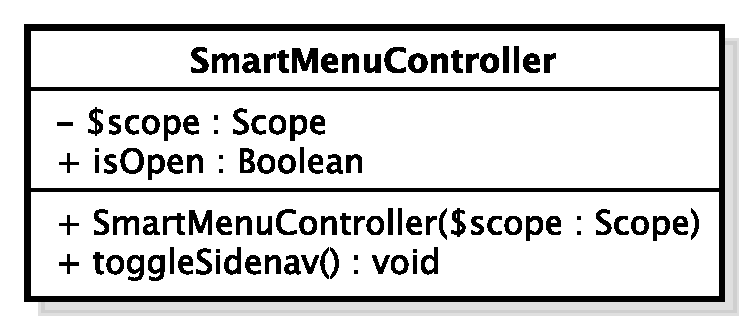
\includegraphics[scale=0.4,keepaspectratio]{diagrammi/classi/{frontEnd/controllers/SmartMenuController}.pdf}}
\caption{\nogloxy{Premi::Front-End::Controllers::SmartMenuController}}
\end{figure}
\FloatBarrier
\begin{itemize}
\item \textbf{Descrizione}\\
Classe che gestisce la visibilità della directive \texttt{premiSmartMenu}.
\item \textbf{Utilizzo}\\
Viene utilizzata per permettere all'utente di nascondere il menù con i nodi associati al nodo visualizzato in presentazione.
\item \textbf{Relazioni con altre classi}:
\begin{itemize}
\item \textit{OUT} \hyperref[\nogloxy{Premi::Front-End::Directives::premiSmartMenu}]{\nogloxy{\texttt{premiSmartMenu}}}\\
Rappresenta il menù che durante la presentazione permette di navigare la \gloxy{mappa mentale} seguendo le associazioni definite tra i vari nodi.
Questo componente consiste in una lista di elementi selezionabili dall’utente, ogni elemento corrisponde ad un'associazione presente tra il nodo corrente ed un altro nodo della mappa.
\end{itemize}
\item \textbf{Attributi}:
\begin{itemize}
\item \nogloxy{\texttt{+ isOpen: Boolean}}
\\ Campo dati che specifica se il menù è aperto o chiuso.
\item \nogloxy{\texttt{- \$scope: Scope}}
\\ \dpScopeField
\end{itemize}
\item \textbf{Metodi}:
\begin{itemize}
\item \nogloxy{\texttt{+ SmartMenuController(\$scope: Scope)}}
\\ \dpConstructor
\\ \textbf{Parametri}:
\begin{itemize}
\item \nogloxy{\texttt{\$scope: Scope}}
\\ \dpScopeParam
\end{itemize}
\item \nogloxy{\texttt{+ toggleSidenav(): void}}
\\ Metodo che inverte il valore del campo dati \texttt{isOpen}.
\end{itemize}
\end{itemize}
\subsection{\nogloxy{Premi::Front-End::Directives}}
\label{\nogloxy{Premi::Front-End::Directives}}
\subsubsection{Informazioni generali}
\begin{figure}[h]
\centering
\nogloxy{\includegraphics[scale=0.4,keepaspectratio]{diagrammi/package/{frontEnd-directives}.pdf}}
\caption{\nogloxy{Premi::Front-End::Directives}}
\end{figure}
\FloatBarrier
\begin{itemize}
\item \textbf{Descrizione}\\
Package contenente le directives che compongno le views.
\item \textbf{Padre}: \hyperref[\nogloxy{Premi::Front-End}]{\nogloxy{\texttt{Front-End}}}
\item \textbf{Interazioni con altri componenti}:
\begin{itemize}
\item \hyperref[\nogloxy{Premi::Front-End::Controllers}]{\nogloxy{\texttt{Controllers}}}\\
Package contenente i \gloxy{controller} della componente \gloxy{front-end} dell’applicazione.
\item \hyperref[\nogloxy{Premi::Front-End::Model}]{\nogloxy{\texttt{Model}}}\\
Package contenente le classi che definiscono la \gloxy{business logic} dell’applicazione.
\item \hyperref[\nogloxy{Premi::Front-End::Views}]{\nogloxy{\texttt{Views}}}\\
Package contenente le views della componente \gloxy{front-end} dell’applicazione.
\end{itemize}
\end{itemize}
\subsubsection{Classi}
\subsubsubsection{\nogloxy{Premi::Front-End::Directives::premiAddToPath}}
\label{\nogloxy{Premi::Front-End::Directives::premiAddToPath}}
\begin{figure}[h]
\centering
\nogloxy{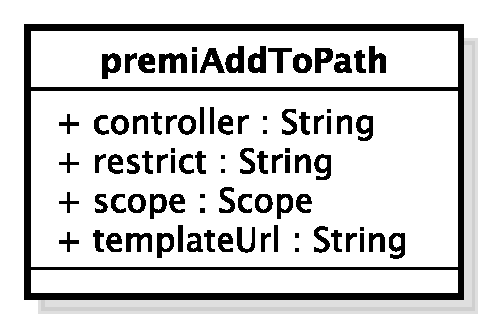
\includegraphics[scale=0.4,keepaspectratio]{diagrammi/classi/{frontEnd/directives/premiAddToPath}.pdf}}
\caption{\nogloxy{Premi::Front-End::Directives::premiAddToPath}}
\end{figure}
\FloatBarrier
\begin{itemize}
\item \textbf{Descrizione}\\
Rappresenta il componente grafico che permette all’utente di visualizzare il contenuto di un nodo e di aggiungerlo ad uno dei \gloxy{percorsi di presentazione} esistenti.
Questo componente visualizza una lista contenente tutti i \gloxy{percorsi} disponibili al quale, selezionando quello desiderato, è possibile aggiungere il nodo slezionato.
\item \textbf{Utilizzo}\\
Viene utilizzato per consentire all’utente di aggiungere un nodo ad un \gloxy{percorso} di presentazione.
\item \textbf{Relazioni con altre classi}:
\begin{itemize}
\item \textit{IN} \hyperref[\nogloxy{Premi::Front-End::Controllers::AddToPathController}]{\nogloxy{\texttt{AddToPathController}}}\\
Classe che si occupa di gestire la logica di funzionamento della directive \texttt{premiAddToPath}.
\item \textit{IN} \hyperref[\nogloxy{Premi::Front-End::Views::PathsEditorView}]{\nogloxy{\texttt{PathsEditorView}}}\\
\gloxy{View} dell’applicazione contenente la mappa mentale. Offre funzionalità legate ai \gloxy{percorsi} di presentazione.
Da questa \gloxy{view} è possibile:
\begin{itemize}
\item Creare/eliminare un \gloxy{percorso} di presentazione;
\item Modificare un \gloxy{percorso} aggiungendo e togliendo nodi, oppure rinominandolo;
\item Scegliere un \gloxy{percorso} da presentare e successivamente presentarlo.
\end{itemize}
\item \textit{OUT} \hyperref[\nogloxy{Premi::Front-End::Directives::premiNode}]{\nogloxy{\texttt{premiNode}}}\\
Rappresenta il componente grafico che visualizza il contenuto di un nodo. Questo contenuto non deve essere modificabile.
\item \textit{OUT} \hyperref[\nogloxy{Premi::Front-End::Model::Node}]{\nogloxy{\texttt{Node}}}\\
Rappresenta un nodo della mappa mentale. Contiene tutte le informazioni necessarie alla presentazione del contenuto del nodo.
\end{itemize}
\item \textbf{Attributi}:
\begin{itemize}
\item \nogloxy{\texttt{+ controller: String}}
\\ \dpDirectiveController
\item \nogloxy{\texttt{+ restrict: String}}
\\ \dpRestrict
\item \nogloxy{\texttt{+ scope: Scope}}
\\ \dpIsolatedScope \\
Lo scope deve contenere i seguenti oggetti:
\begin{itemize}
\item \texttt{node (=)}: oggetto di tipo \texttt{Node} contenente i dati del nodo che si vuole aggiungere al \gloxy{percorso};
\item \texttt{paths (=)}: oggetto contenente le informazioni riguardanti i \gloxy{percorsi} presenti all'interno del \gloxy{progetto}. Queste informazioni sono memorizzate come coppie chiave/valore, usando l'\texttt{id} del \gloxy{percorso} come chiave e il nome come valore;
\item \texttt{onAdd (\&)}: funzione da invocare quanto l’utente conferma l’inserimento di un nodo in un \gloxy{percorso}. La funzione viene invocata con due parametri di tipo stringa rappresentanti l’id del nodo e l’id del \gloxy{percorso} in cui inserirlo.
\end{itemize}
\item \nogloxy{\texttt{+ templateUrl: String}}
\\ \dpTemplateUrl
\end{itemize}
\end{itemize}
\subsubsubsection{\nogloxy{Premi::Front-End::Directives::premiAssociationAdder}}
\label{\nogloxy{Premi::Front-End::Directives::premiAssociationAdder}}
\begin{figure}[h]
\centering
\nogloxy{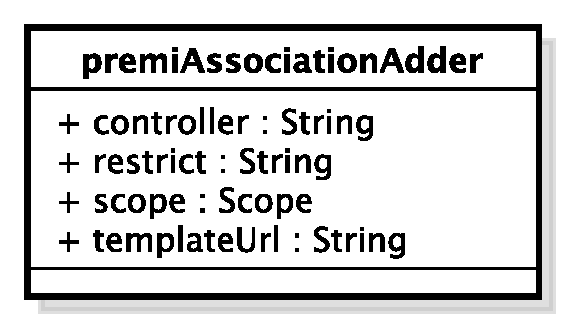
\includegraphics[scale=0.4,keepaspectratio]{diagrammi/classi/{frontEnd/directives/premiAssociationAdder}.pdf}}
\caption{\nogloxy{Premi::Front-End::Directives::premiAssociationAdder}}
\end{figure}
\FloatBarrier
\begin{itemize}
\item \textbf{Descrizione}\\
Rappresenta il componente grafico che permette all’utente di creare un'associazione tra il nodo selezionato e un altro nodo della mappa.
\item \textbf{Utilizzo}\\
Viene utilizzata per consentire all’utente di aggiungere un'associazione tra il nodo selezionato ed un altro nodo della mappa.
\item \textbf{Relazioni con altre classi}:
\begin{itemize}
\item \textit{IN} \hyperref[\nogloxy{Premi::Front-End::Controllers::AssociationAdderController}]{\nogloxy{\texttt{AssociationAdderController}}}\\
Classe che gestisce il funzionamento della directive \texttt{premiAssociationAdder}.
\item \textit{IN} \hyperref[\nogloxy{Premi::Front-End::Views::MindmapEditorView}]{\nogloxy{\texttt{MindmapEditorView}}}\\
\gloxy{View} dell’applicazione contenente la mappa mentale. Offre funzionalità di modifica della mappa.
Da questa \gloxy{view} è possibile:
\begin{itemize}
\item Aggiungere/togliere nodi;
\item Modificare il contenuto di un nodo;
\item Aggiungere/togliere associazioni tra nodi;
\item Modificare i parametri del \gloxy{progetto}.
\end{itemize}
\end{itemize}
\item \textbf{Attributi}:
\begin{itemize}
\item \nogloxy{\texttt{+ controller: String}}
\\ \dpDirectiveController
\item \nogloxy{\texttt{+ restrict: String}}
\\ \dpRestrict
\item \nogloxy{\texttt{+ scope: Scope}}
\\ \dpIsolatedScope \\
Lo scope deve contenere i seguenti oggetti:
\begin{itemize}
\item \texttt{nodes (=)}: oggetto contenente le informazioni riguardanti i nodi con i quali è possibile definire un'associazione, le informazioni sono memorizzate come coppie chiave/valore, usando come chiave l'texttt{id} del nodo e come valore il titolo;
\item \texttt{onNodeSelected (\&)}: funzione da invocare quando l’utente seleziona un nodo tra quelli disponibili, la funzione viene invocata con un parametro di tipo stringa corrispondente all’id del nodo selezionato.
\end{itemize}
\item \nogloxy{\texttt{+ templateUrl: String}}
\\ \dpTemplateUrl
\end{itemize}
\end{itemize}
\subsubsubsection{\nogloxy{Premi::Front-End::Directives::premiContextMenu}}
\label{\nogloxy{Premi::Front-End::Directives::premiContextMenu}}
\begin{figure}[h]
\centering
\nogloxy{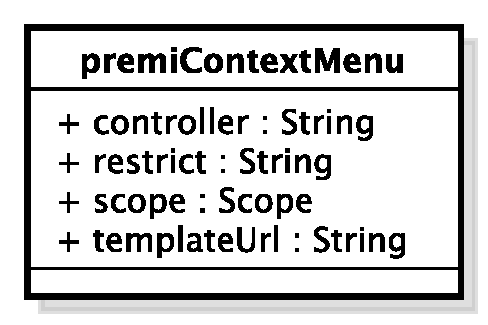
\includegraphics[scale=0.4,keepaspectratio]{diagrammi/classi/{frontEnd/directives/premiContextMenu}.pdf}}
\caption{\nogloxy{Premi::Front-End::Directives::premiContextMenu}}
\end{figure}
\FloatBarrier
\begin{itemize}
\item \textbf{Descrizione}\\
Rappresenta un menù contestuale generato in base agli oggetti passati nello scope isolato. Fornisce un pulsante per ogni oggetto ricevuto come parametro, ogni pulsante viene rappresentato con un'icona e con del testo. Al click di un pulsante viene invocata la funzione ad esso associata.
\item \textbf{Utilizzo}\\
Viene utilizzato per realizzare i menù che vengono visualizzati quando l'utente seleziona un nodo o una relazione presente nella mappa.
\item \textbf{Relazioni con altre classi}:
\begin{itemize}
\item \textit{IN} \hyperref[\nogloxy{Premi::Front-End::Controllers::ContextMenuController}]{\nogloxy{\texttt{ContextMenuController}}}\\
Classe che gestisce il comportamento della directive \texttt{premiContextMenu}.
\item \textit{IN} \hyperref[\nogloxy{Premi::Front-End::Views::MindmapEditorView}]{\nogloxy{\texttt{MindmapEditorView}}}\\
\gloxy{View} dell’applicazione contenente la mappa mentale. Offre funzionalità di modifica della mappa.
Da questa \gloxy{view} è possibile:
\begin{itemize}
\item Aggiungere/togliere nodi;
\item Modificare il contenuto di un nodo;
\item Aggiungere/togliere associazioni tra nodi;
\item Modificare i parametri del \gloxy{progetto}.
\end{itemize}
\item \textit{OUT} \hyperref[\nogloxy{Premi::Front-End::Directives::premiNode}]{\nogloxy{\texttt{premiNode}}}\\
Rappresenta il componente grafico che visualizza il contenuto di un nodo. Questo contenuto non deve essere modificabile.
\end{itemize}
\item \textbf{Attributi}:
\begin{itemize}
\item \nogloxy{\texttt{+ controller: String}}
\\ \dpDirectiveController
\item \nogloxy{\texttt{+ restrict: String}}
\\ \dpRestrict
\item \nogloxy{\texttt{+ scope: Scope}}
\\ \dpIsolatedScope \\
Lo scope deve contenere i seguenti oggetti:
\begin{itemize}
\item \texttt{\gloxy{objectId} (@)}: stringa contenente l'id dell'oggetto sul quale viene visualizzato il menù;
\item \texttt{node (=)}: (opzionale) oggetto di tipo \texttt{Node} del quale visualizzare l'anteprima;
\item \texttt{operations (=)}: \texttt{Array} di oggetti contenenti i seguenti campi dati:
\begin{itemize}
\item \texttt{name}: stringa contenente il nome da visualizzare;
\item \texttt{\gloxy{callback}}: funzione da eseguire quando l'utente seleziona la voce del menù, viene invocata con \texttt{\gloxy{objectId}} come parametro;
\item \texttt{image}: stringa contenente l'URL dell'immagine da visualizzare di fianco alla voce del menù.
\end{itemize}
\end{itemize}
\item \nogloxy{\texttt{+ templateUrl: String}}
\\ \dpTemplateUrl
\end{itemize}
\end{itemize}
\subsubsubsection{\nogloxy{Premi::Front-End::Directives::premiEditableNodeContent}}
\label{\nogloxy{Premi::Front-End::Directives::premiEditableNodeContent}}
\begin{figure}[h]
\centering
\nogloxy{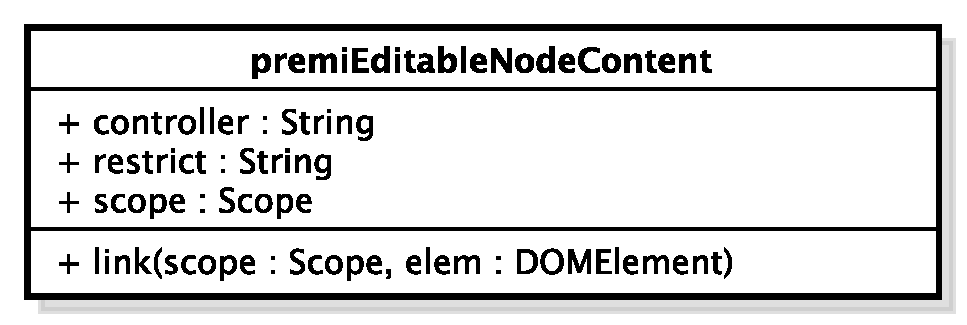
\includegraphics[scale=0.4,keepaspectratio]{diagrammi/classi/{frontEnd/directives/premiEditableNodeContent}.pdf}}
\caption{\nogloxy{Premi::Front-End::Directives::premiEditableNodeContent}}
\end{figure}
\FloatBarrier
\begin{itemize}
\item \textbf{Descrizione}\\
Rappresenta un elemento contenuto nel \gloxy{frame} di un nodo. Questo elemento è spostabile e ridimensionabile. Le modifiche effettuate su questo elemento vengono riportate direttamente sull’oggetto \texttt{nodeContent}.
Questo componente deve essere in grado di rappresentare le varie tipologie di contenuto che possono essere presenti all’interno di un nodo. La discriminazione del tipo del contenuto deve essere fatta in base ai campi dati dell’oggetto \texttt{nodeContent}.
\item \textbf{Utilizzo}\\
Viene utilizzato per permettere all'utente di spostare un elemento contenuto all'interno di un \gloxy{frame}.
\item \textbf{Relazioni con altre classi}:
\begin{itemize}
\item \textit{IN} \hyperref[\nogloxy{Premi::Front-End::Controllers::EditableNodeContentController}]{\nogloxy{\texttt{EditableNodeContentController}}}\\
Classe che gestisce la logica della directive \texttt{premiEditableNodeContent}. Questa classe registra un gestore per l'evento \texttt{nodecontent-deselect} che imposta come de-selezionata la directive.
\item \textit{IN} \hyperref[\nogloxy{Premi::Front-End::Directives::premiNodeContentsEditor}]{\nogloxy{\texttt{premiNodeContentsEditor}}}\\
Rappresenta il componente grafico che permette all’utente di modificare il contenuto di un nodo. Questo componente fornisce all’utente sia dei campi per inserire/modificare il contenuto del nodo, sia un’anteprima di come questo verrà visualizzato. Dall’anteprima sarà anche possibile spostare e ridimensionare i vari componenti.
Saranno presenti inoltre due pulsanti, uno per confermare le modifiche e l’altro per annullarle e ripristinare lo stato del nodo.
\item \textit{OUT} \hyperref[\nogloxy{Premi::Front-End::Model::NodeContent}]{\nogloxy{\texttt{NodeContent}}}\\
Rappresenta il contenuto di un nodo. Contiene informazioni che indicano deve essere visualizzato il contenuto all’interno del nodo.
\end{itemize}
\item \textbf{Attributi}:
\begin{itemize}
\item \nogloxy{\texttt{+ controller: String}}
\\ \dpDirectiveController
\item \nogloxy{\texttt{+ restrict: String}}
\\ \dpRestrict
\item \nogloxy{\texttt{+ scope: Scope}}
\\ \dpIsolatedScope \\
Dentro questo oggetto devono essere presenti i seguenti oggetti:
\begin{itemize}
\item \texttt{nodeContent (=)}: oggetto che rappresenta un elemento contenuto nel \gloxy{frame} di un nodo;
\item \texttt{container (=)}: oggetto contenente le informazioni riguardanti le dimensioni del contenitore della directive, in particolare l'oggetto ha due campi dati: \texttt{width} e \texttt{height}.
\end{itemize}
\end{itemize}
\item \textbf{Metodi}:
\begin{itemize}
\item \nogloxy{\texttt{+ link(scope: Scope, elem: DOMElement)}}
\\ \dpLinkFn \\ Viene utilizzata per registrare i vari gestori degli eventi del mouse in modo da poter effettuare il \textit{drag'n'drop} e vengono aggiunti ulteriori elementi al DOM per poter effettuare il ridimensionamento dell'elemento.
\\ \textbf{Parametri}:
\begin{itemize}
\item \nogloxy{\texttt{scope: Scope}}
\\ Parametro che contiene un riferimento all'oggetto \texttt{scope} della directive.
\item \nogloxy{\texttt{elem: DOMElement}}
\\ Parametro contenente un oggetto della \gloxy{libreria} jQuery che rappresenta l'oggetto del DOM sul quale è definita la directive.
\end{itemize}
\end{itemize}
\end{itemize}
\subsubsubsection{\nogloxy{Premi::Front-End::Directives::premiErrorMessage}}
\label{\nogloxy{Premi::Front-End::Directives::premiErrorMessage}}
\begin{figure}[h]
\centering
\nogloxy{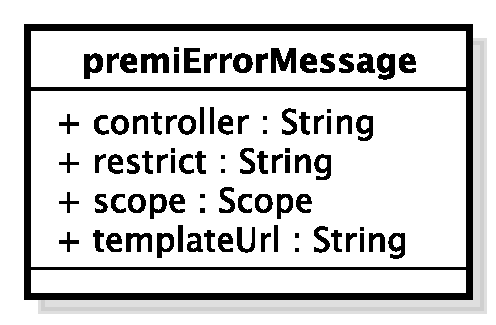
\includegraphics[scale=0.4,keepaspectratio]{diagrammi/classi/{frontEnd/directives/premiErrorMessage}.pdf}}
\caption{\nogloxy{Premi::Front-End::Directives::premiErrorMessage}}
\end{figure}
\FloatBarrier
\begin{itemize}
\item \textbf{Descrizione}\\
Rappresenta il componente grafico che permette di mostrare messaggi d’errore all’utente all’interno dell’applicazione. Questo componente fornisce anche un pulsante che permette di nascondere il messaggio.
\item \textbf{Utilizzo}\\
Viene utilizzato per comunicare all’utente gli errori relativi ai dati inseriti o ad operazioni non consentite che l’utente cerca di effetturare.
\item \textbf{Relazioni con altre classi}:
\begin{itemize}
\item \textit{IN} \hyperref[\nogloxy{Premi::Front-End::AppRun}]{\nogloxy{\texttt{AppRun}}}\\
Classe che si occupa di gestire l'inizializzazione dell'applicazione.
\item \textit{IN} \hyperref[\nogloxy{Premi::Front-End::Controllers::ErrorMessageController}]{\nogloxy{\texttt{ErrorMessageController}}}\\
Classe che gestisce la logica di visualizzazione della directive \texttt{premiErrorMessage}.
\item \textit{OUT} \hyperref[\nogloxy{Premi::Front-End::Model::ErrorInfo}]{\nogloxy{\texttt{ErrorInfo}}}\\
Rappresenta le informazioni di un errore che si è verificato eseguendo una determinata operazione.
\end{itemize}
\item \textbf{Attributi}:
\begin{itemize}
\item \nogloxy{\texttt{+ controller: String}}
\\ \dpDirectiveController
\item \nogloxy{\texttt{+ restrict: String}}
\\ \dpRestrict
\item \nogloxy{\texttt{+ scope: Scope}}
\\ \dpIsolatedScope \\
Lo scope riceve un oggetto di tipo \texttt{ErrorInfo} contenente tutte le informazioni riguardanti l'errore che si è verificato.
\item \nogloxy{\texttt{+ templateUrl: String}}
\\ \dpTemplateUrl
\end{itemize}
\end{itemize}
\subsubsubsection{\nogloxy{Premi::Front-End::Directives::premiHeader}}
\label{\nogloxy{Premi::Front-End::Directives::premiHeader}}
\begin{figure}[h]
\centering
\nogloxy{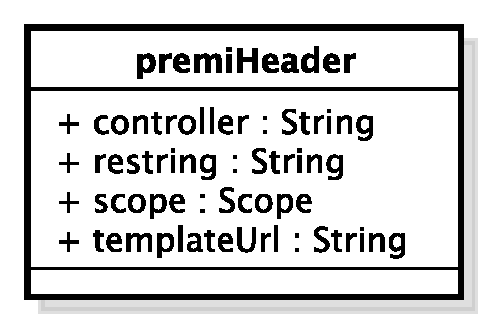
\includegraphics[scale=0.4,keepaspectratio]{diagrammi/classi/{frontEnd/directives/premiHeader}.pdf}}
\caption{\nogloxy{Premi::Front-End::Directives::premiHeader}}
\end{figure}
\FloatBarrier
\begin{itemize}
\item \textbf{Descrizione}\\
Rappresenta la barra di navigazione che permette all’utente di spostarsi tra le varie views dell'applicazione. Fornisce inoltre i pulsanti per visualizzare il manuale utente, effettuare il logout, chiudere al presentazione e il \gloxy{progetto}. Inoltre, quando l'utente si trova nelle views in cui è possibile modificare il \gloxy{progetto}, questa directive permette di mostrare la finestra di modifica delle impostazioni del \gloxy{progetto}, sia di interagire con la visualizzazione della mappa mentale, modificando lo zoom e permettendo anche di stamparla.
\item \textbf{Utilizzo}\\
Viene utilizzata per consentire all’utente di spostarsi tra la varie views dell’applicazione, per effettuare il logout e per accedere al manuale dell'applicazione.
\item \textbf{Relazioni con altre classi}:
\begin{itemize}
\item \textit{IN} \hyperref[\nogloxy{Premi::Front-End::Controllers::HeaderController}]{\nogloxy{\texttt{HeaderController}}}\\
Classe che gestisce le operazioni e la logica applicativa della directive \texttt{premiHeader},
\item \textit{IN} \hyperref[\nogloxy{Premi::Front-End::Views::MindmapEditorView}]{\nogloxy{\texttt{MindmapEditorView}}}\\
\gloxy{View} dell’applicazione contenente la mappa mentale. Offre funzionalità di modifica della mappa.
Da questa \gloxy{view} è possibile:
\begin{itemize}
\item Aggiungere/togliere nodi;
\item Modificare il contenuto di un nodo;
\item Aggiungere/togliere associazioni tra nodi;
\item Modificare i parametri del \gloxy{progetto}.
\end{itemize}
\item \textit{IN} \hyperref[\nogloxy{Premi::Front-End::Views::PathsEditorView}]{\nogloxy{\texttt{PathsEditorView}}}\\
\gloxy{View} dell’applicazione contenente la mappa mentale. Offre funzionalità legate ai \gloxy{percorsi} di presentazione.
Da questa \gloxy{view} è possibile:
\begin{itemize}
\item Creare/eliminare un \gloxy{percorso} di presentazione;
\item Modificare un \gloxy{percorso} aggiungendo e togliendo nodi, oppure rinominandolo;
\item Scegliere un \gloxy{percorso} da presentare e successivamente presentarlo.
\end{itemize}
\item \textit{OUT} \hyperref[\nogloxy{Premi::Front-End::Directives::premiProjectSettingsEditor}]{\nogloxy{\texttt{premiProjectSettingsEditor}}}\\
Rappresenta il componente grafico che permette di modificare i dati del \gloxy{progetto} aperto.
Questo componente presenta i vari campi per interagire con i parametri del \gloxy{progetto} e due pulsanti che l'utente utilizza per confermare o annullare le modifiche.
\end{itemize}
\item \textbf{Attributi}:
\begin{itemize}
\item \nogloxy{\texttt{+ controller: String}}
\\ \dpDirectiveController
\item \nogloxy{\texttt{+ restrict: String}}
\\ \dpRestrict
\item \nogloxy{\texttt{+ scope: Scope}}
\\ \dpIsolatedScope
\item \nogloxy{\texttt{+ templateUrl: String}}
\\ \dpTemplateUrl
\end{itemize}
\end{itemize}
\subsubsubsection{\nogloxy{Premi::Front-End::Directives::premiHierarchicalMenu}}
\label{\nogloxy{Premi::Front-End::Directives::premiHierarchicalMenu}}
\begin{figure}[h]
\centering
\nogloxy{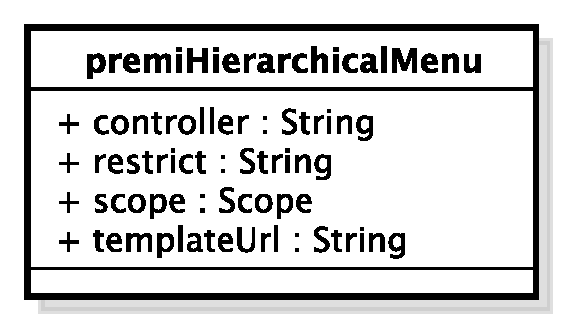
\includegraphics[scale=0.4,keepaspectratio]{diagrammi/classi/{frontEnd/directives/premiHierarchicalMenu}.pdf}}
\caption{\nogloxy{Premi::Front-End::Directives::premiHierarchicalMenu}}
\end{figure}
\FloatBarrier
\begin{itemize}
\item \textbf{Descrizione}\\
Rappresenta il menù che durante la presentazione permette di navigare la \gloxy{mappa mentale} seguendo le relazioni gerarchiche presenti tra i vari nodi della mappa mentale. Questo componente consiste in una lista di elementi selezionabili dall’utente, ogni elemento corrisponde ad una relazione presente tra il nodo corrente ed un altro nodo della mappa.
\item \textbf{Utilizzo}\\
Viene utilizzata per permettere all'utente di spostarsi tra i nodi della \gloxy{mappa mentale} seguendo le relazioni gerarchiche presenti.
\item \textbf{Relazioni con altre classi}:
\begin{itemize}
\item \textit{IN} \hyperref[\nogloxy{Premi::Front-End::Controllers::HierarchicalMenuController}]{\nogloxy{\texttt{HierarchicalMenuController}}}\\
Classe che gestisce la visibilità della directive \texttt{premiHierarchicalMenu}.
\item \textit{IN} \hyperref[\nogloxy{Premi::Front-End::Views::PresentationView}]{\nogloxy{\texttt{PresentationView}}}\\
\gloxy{View} dell’applicazione che permette di effettuare la presentazione di un \gloxy{percorso} scelto dall’utente. Utilizza la directive \texttt{premiPresentation} per offrire funzionalità legate alla presentazione lineare e due menù per permettere all'utente di spostarsi in modo non lineare, seguendo le relazioni definite tra i nodi della mappa mentale.
Da questa vista è inoltre possibile stampare ed esportare il \gloxy{percorso di presentazione} in esecuzione, mediante le funzionalità offerte dal \gloxy{browser}.
\item \textit{OUT} \hyperref[\nogloxy{Premi::Front-End::Model::NodeReference}]{\nogloxy{\texttt{NodeReference}}}\\
Rappresenta il riferimento ad un nodo della mappa mentale, contiene l'identificativo e il titolo del del nodo.
\end{itemize}
\item \textbf{Attributi}:
\begin{itemize}
\item \nogloxy{\texttt{+ controller: String}}
\\ \dpDirectiveController
\item \nogloxy{\texttt{+ restrict: String}}
\\ \dpRestrict
\item \nogloxy{\texttt{+ scope: Scope}}
\\ \dpIsolatedScope \\
Lo scope deve contenere i seguenti oggetti:
\begin{itemize}
\item \texttt{parent (=)}: oggetto di tipo \texttt{NodeReference} contenente un riferimento al nodo padre del nodo correntemente visualizzato;
\item \texttt{relations (=)}: \texttt{Array} contenente oggetti di tipo \texttt{NodeReference}, rappresentanti le associazioni che coinvolgono il nodo correntemente visualizzato;
\item \texttt{onClick (\&)}: funzione da invocare quando l’utente clicca su un elemento del menù. La funzione viene invocata con un parametro corrispondete all’id del nodo che compare nella relazione selezionata dall’utente.
\end{itemize}
\item \nogloxy{\texttt{+ templateUrl: String}}
\\ \dpTemplateUrl
\end{itemize}
\end{itemize}
\subsubsubsection{\nogloxy{Premi::Front-End::Directives::premiMindmap}}
\label{\nogloxy{Premi::Front-End::Directives::premiMindmap}}
\begin{figure}[h]
\centering
\nogloxy{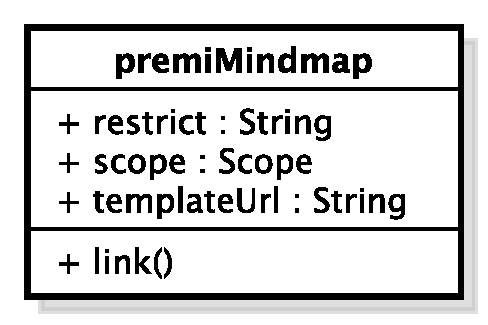
\includegraphics[scale=0.4,keepaspectratio]{diagrammi/classi/{frontEnd/directives/premiMindmap}.pdf}}
\caption{\nogloxy{Premi::Front-End::Directives::premiMindmap}}
\end{figure}
\FloatBarrier
\begin{itemize}
\item \textbf{Descrizione}\\
Rappresenta il componente grafico che disegna la mappa mentale.
\item \textbf{Utilizzo}\\
Viene utilizzato per inserire all'interno delle varie \gloxy{view} dell'applicazione la mappa mentale.
\item \textbf{Relazioni con altre classi}:
\begin{itemize}
\item \textit{IN} \hyperref[\nogloxy{Premi::Front-End::Services::MindmapService}]{\nogloxy{\texttt{MindmapService}}}\\
Questa classe si occupa del recupero e della modifica delle informazioni relative ai nodi e alle associazione presenti nella \gloxy{mappa mentale} del \gloxy{progetto} corrente. Utilizza \texttt{\$http} per comunicare con il \gloxy{back-end} e \texttt{MindmapAdapterService} per memorizzare i dati in locale.
\item \textit{IN} \hyperref[\nogloxy{Premi::Front-End::Views::PathsEditorView}]{\nogloxy{\texttt{PathsEditorView}}}\\
\gloxy{View} dell’applicazione contenente la mappa mentale. Offre funzionalità legate ai \gloxy{percorsi} di presentazione.
Da questa \gloxy{view} è possibile:
\begin{itemize}
\item Creare/eliminare un \gloxy{percorso} di presentazione;
\item Modificare un \gloxy{percorso} aggiungendo e togliendo nodi, oppure rinominandolo;
\item Scegliere un \gloxy{percorso} da presentare e successivamente presentarlo.
\end{itemize}
\end{itemize}
\item \textbf{Attributi}:
\begin{itemize}
\item \nogloxy{\texttt{+ replace: Boolean}}
\\ \dpReplace
\item \nogloxy{\texttt{+ restrict: String}}
\\ \dpRestrict
\item \nogloxy{\texttt{+ scope: Scope}}
\\ \dpIsolatedScope
\item \nogloxy{\texttt{+ templateUrl: String}}
\\ \dpTemplateUrl
\end{itemize}
\item \textbf{Metodi}:
\begin{itemize}
\item \nogloxy{\texttt{+ link()}}
\\ \dpLinkFn \\ Viene utilizzata per disegnare la mappa mentale.
\end{itemize}
\end{itemize}
\subsubsubsection{\nogloxy{Premi::Front-End::Directives::premiNode}}
\label{\nogloxy{Premi::Front-End::Directives::premiNode}}
\begin{figure}[h]
\centering
\nogloxy{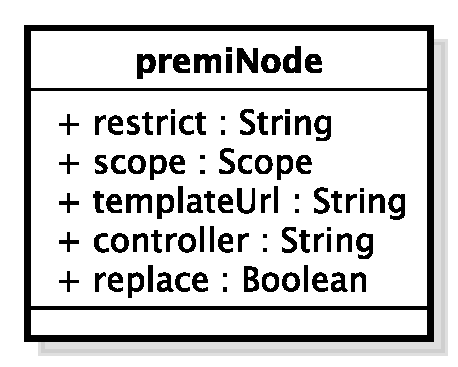
\includegraphics[scale=0.4,keepaspectratio]{diagrammi/classi/{frontEnd/directives/premiNode}.pdf}}
\caption{\nogloxy{Premi::Front-End::Directives::premiNode}}
\end{figure}
\FloatBarrier
\begin{itemize}
\item \textbf{Descrizione}\\
Rappresenta il componente grafico che visualizza il contenuto di un nodo. Questo contenuto non deve essere modificabile.
\item \textbf{Utilizzo}\\
Viene utilizzato per visualizzare il contenuto di un nodo.
\item \textbf{Relazioni con altre classi}:
\begin{itemize}
\item \textit{IN} \hyperref[\nogloxy{Premi::Front-End::Controllers::NodeController}]{\nogloxy{\texttt{NodeController}}}\\
Classe che si occupa di gestire il funzionamento della directive \texttt{premiNode}.
\item \textit{IN} \hyperref[\nogloxy{Premi::Front-End::Directives::premiAddToPath}]{\nogloxy{\texttt{premiAddToPath}}}\\
Rappresenta il componente grafico che permette all’utente di visualizzare il contenuto di un nodo e di aggiungerlo ad uno dei \gloxy{percorsi di presentazione} esistenti.
Questo componente visualizza una lista contenente tutti i \gloxy{percorsi} disponibili al quale, selezionando quello desiderato, è possibile aggiungere il nodo slezionato.
\item \textit{IN} \hyperref[\nogloxy{Premi::Front-End::Directives::premiContextMenu}]{\nogloxy{\texttt{premiContextMenu}}}\\
Rappresenta un menù contestuale generato in base agli oggetti passati nello scope isolato. Fornisce un pulsante per ogni oggetto ricevuto come parametro, ogni pulsante viene rappresentato con un'icona e con del testo. Al click di un pulsante viene invocata la funzione ad esso associata.
\item \textit{OUT} \hyperref[\nogloxy{Premi::Front-End::Directives::premiNodeContent}]{\nogloxy{\texttt{premiNodeContent}}}\\
Rappresenta un elemento contenuto nel \gloxy{frame} di un nodo.
Questo componente deve essere in grado di rappresentare le varie tipologie di contenuto che possono essere presenti all’interno di un nodo.  La discriminazione del tipo del contenuto deve essere fatta in base ai campi dati dell’oggetto \texttt{nodeContent}.
\item \textit{OUT} \hyperref[\nogloxy{Premi::Front-End::Model::Node}]{\nogloxy{\texttt{Node}}}\\
Rappresenta un nodo della mappa mentale. Contiene tutte le informazioni necessarie alla presentazione del contenuto del nodo.
\item \textit{OUT} \hyperref[\nogloxy{Premi::Front-End::Model::PresentationNode}]{\nogloxy{\texttt{PresentationNode}}}\\
Classe che estende \texttt{Node}, riproducendo una struttura comoda per poter presentare i contenuti di un nodo e semplificare lo spostamento fra \gloxy{frame} associati e con relazioni di tipo gerarchico.
\end{itemize}
\item \textbf{Attributi}:
\begin{itemize}
\item \nogloxy{\texttt{- controller: String}}
\\ \dpDirectiveController
\item \nogloxy{\texttt{+ replace: Boolean}}
\\ \dpReplace
\item \nogloxy{\texttt{+ restrict: String}}
\\ \dpRestrict
\item \nogloxy{\texttt{+ scope: Scope}}
\\ \dpIsolatedScope \\ Dentro questo oggetto devono essere presenti i seguenti oggetti: \begin{itemize} \item \texttt{node (=)}: oggetto di tipo \texttt{Node} che deve essere visualizzato. \end{itemize}
\item \nogloxy{\texttt{+ templateUrl: String}}
\\ \dpTemplateUrl
\end{itemize}
\end{itemize}
\subsubsubsection{\nogloxy{Premi::Front-End::Directives::premiNodeContent}}
\label{\nogloxy{Premi::Front-End::Directives::premiNodeContent}}
\begin{figure}[h]
\centering
\nogloxy{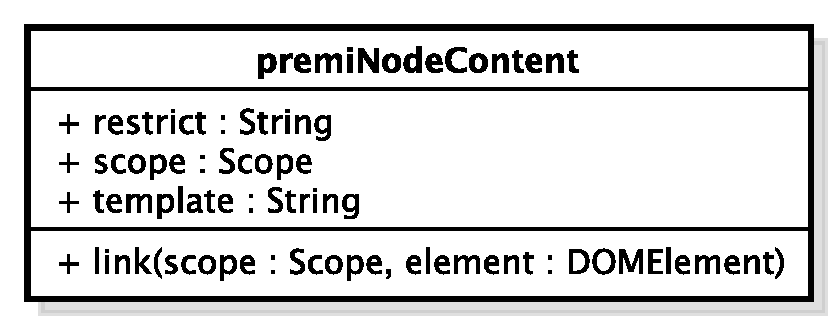
\includegraphics[scale=0.4,keepaspectratio]{diagrammi/classi/{frontEnd/directives/premiNodeContent}.pdf}}
\caption{\nogloxy{Premi::Front-End::Directives::premiNodeContent}}
\end{figure}
\FloatBarrier
\begin{itemize}
\item \textbf{Descrizione}\\
Rappresenta un elemento contenuto nel \gloxy{frame} di un nodo.
Questo componente deve essere in grado di rappresentare le varie tipologie di contenuto che possono essere presenti all’interno di un nodo.  La discriminazione del tipo del contenuto deve essere fatta in base ai campi dati dell’oggetto \texttt{nodeContent}.
\item \textbf{Utilizzo}\\
Viene utilizzata per rappresentare un elemento all'interno del \gloxy{frame} di un nodo.
\item \textbf{Relazioni con altre classi}:
\begin{itemize}
\item \textit{IN} \hyperref[\nogloxy{Premi::Front-End::Directives::premiNode}]{\nogloxy{\texttt{premiNode}}}\\
Rappresenta il componente grafico che visualizza il contenuto di un nodo. Questo contenuto non deve essere modificabile.
\item \textit{OUT} \hyperref[\nogloxy{Premi::Front-End::Model::NodeContent}]{\nogloxy{\texttt{NodeContent}}}\\
Rappresenta il contenuto di un nodo. Contiene informazioni che indicano deve essere visualizzato il contenuto all’interno del nodo.
\end{itemize}
\item \textbf{Attributi}:
\begin{itemize}
\item \nogloxy{\texttt{+ restrict: String}}
\\ \dpRestrict
\item \nogloxy{\texttt{+ scope: Scope}}
\\ \dpIsolatedScope \\
Dentro questo oggetto deve essere presente il seguente oggetto:
\begin{itemize}
\item \texttt{nodeContent (=)}: oggetto di tipo \texttt{NodeContent} che rappresenta un elemento contenuto nel \gloxy{frame} di un nodo.
\end{itemize}
\item \nogloxy{\texttt{+ template: String}}
\\ \dpTemplate
\end{itemize}
\item \textbf{Metodi}:
\begin{itemize}
\item \nogloxy{\texttt{+ link(scope: Scope, element: DOMElement)}}
\\ \dpLinkFn \\ Viene utilizzata per creare l'elemento del DOM corretto in base al tipo di contenuto dell'oggetto e per gestire l'evento \texttt{resize} della pagina.
\\ \textbf{Parametri}:
\begin{itemize}
\item \nogloxy{\texttt{scope: Scope}}
\\ Parametro contenente un riferimento allo \texttt{scope} della directive.
\item \nogloxy{\texttt{element: DOMElement}}
\\ Parametro contenente un oggetto della \gloxy{libreria} jQuery rappresentante l'elemento del DOM contenente la directive.
\end{itemize}
\end{itemize}
\end{itemize}
\subsubsubsection{\nogloxy{Premi::Front-End::Directives::premiNodeContentsEditor}}
\label{\nogloxy{Premi::Front-End::Directives::premiNodeContentsEditor}}
\begin{figure}[h]
\centering
\nogloxy{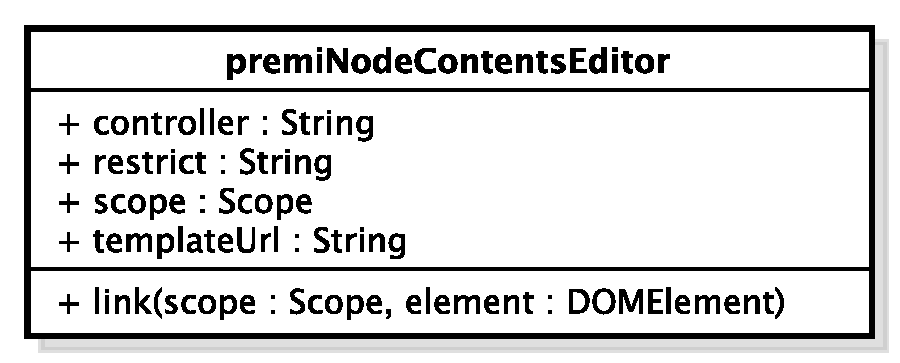
\includegraphics[scale=0.4,keepaspectratio]{diagrammi/classi/{frontEnd/directives/premiNodeContentsEditor}.pdf}}
\caption{\nogloxy{Premi::Front-End::Directives::premiNodeContentsEditor}}
\end{figure}
\FloatBarrier
\begin{itemize}
\item \textbf{Descrizione}\\
Rappresenta il componente grafico che permette all’utente di modificare il contenuto di un nodo. Questo componente fornisce all’utente sia dei campi per inserire/modificare il contenuto del nodo, sia un’anteprima di come questo verrà visualizzato. Dall’anteprima sarà anche possibile spostare e ridimensionare i vari componenti.
Saranno presenti inoltre due pulsanti, uno per confermare le modifiche e l’altro per annullarle e ripristinare lo stato del nodo.
\item \textbf{Utilizzo}\\
Viene utilizzata per permettere all’utente di modificare i nodi della mappa menale.
\item \textbf{Relazioni con altre classi}:
\begin{itemize}
\item \textit{IN} \hyperref[\nogloxy{Premi::Front-End::Controllers::NodeContentsEditorController}]{\nogloxy{\texttt{NodeContentsEditorController}}}\\
Classe che si occupa di gestire la logica legata alla modifica del contenuto di un nodo.
\item \textit{IN} \hyperref[\nogloxy{Premi::Front-End::Views::MindmapEditorView}]{\nogloxy{\texttt{MindmapEditorView}}}\\
\gloxy{View} dell’applicazione contenente la mappa mentale. Offre funzionalità di modifica della mappa.
Da questa \gloxy{view} è possibile:
\begin{itemize}
\item Aggiungere/togliere nodi;
\item Modificare il contenuto di un nodo;
\item Aggiungere/togliere associazioni tra nodi;
\item Modificare i parametri del \gloxy{progetto}.
\end{itemize}
\item \textit{OUT} \hyperref[\nogloxy{Premi::Front-End::Directives::premiEditableNodeContent}]{\nogloxy{\texttt{premiEditableNodeContent}}}\\
Rappresenta un elemento contenuto nel \gloxy{frame} di un nodo. Questo elemento è spostabile e ridimensionabile. Le modifiche effettuate su questo elemento vengono riportate direttamente sull’oggetto \texttt{nodeContent}.
Questo componente deve essere in grado di rappresentare le varie tipologie di contenuto che possono essere presenti all’interno di un nodo. La discriminazione del tipo del contenuto deve essere fatta in base ai campi dati dell’oggetto \texttt{nodeContent}.
\item \textit{OUT} \hyperref[\nogloxy{Premi::Front-End::Model::Node}]{\nogloxy{\texttt{Node}}}\\
Rappresenta un nodo della mappa mentale. Contiene tutte le informazioni necessarie alla presentazione del contenuto del nodo.
\end{itemize}
\item \textbf{Attributi}:
\begin{itemize}
\item \nogloxy{\texttt{+ controller: String}}
\\ \dpDirectiveController
\item \nogloxy{\texttt{+ restrict: String}}
\\ \dpRestrict
\item \nogloxy{\texttt{+ scope: Scope}}
\\ \dpIsolatedScope \\
All'interno dello scope dovranno essere presenti i seguenti oggetti:
\begin{itemize}
\item \texttt{node (=)}: oggetto di tipo nodo che deve essere modificato;
\item \texttt{onConfirm (\&)}: funzione invocata quando l’utente conferma le modifiche effettuate;
\item \texttt{onReset (\&)}: funzione invocata quando l’utente decide di annullare le modifiche.
\end{itemize}
\item \nogloxy{\texttt{+ templateUrl: String}}
\\ \dpTemplateUrl
\end{itemize}
\item \textbf{Metodi}:
\begin{itemize}
\item \nogloxy{\texttt{+ link(scope: Scope, element: DOMElement)}}
\\ \dpLinkFn \\ Viene utilizzata per registrare un gestore per l'evento \texttt{resize} del \gloxy{browser}, in modo da poter scalare in modo corretto i contenuti del nodo.
\\ \textbf{Parametri}:
\begin{itemize}
\item \nogloxy{\texttt{scope: Scope}}
\\ Parametro contenente un riferimento allo \texttt{scope} della directive.
\item \nogloxy{\texttt{element: DOMElement}}
\\ Parametro contenente un oggetto della \gloxy{libreria} jQuery rappresentante l'elemento del DOM contenente la directive.
\end{itemize}
\end{itemize}
\end{itemize}
\subsubsubsection{\nogloxy{Premi::Front-End::Directives::premiPath}}
\label{\nogloxy{Premi::Front-End::Directives::premiPath}}
\begin{figure}[h]
\centering
\nogloxy{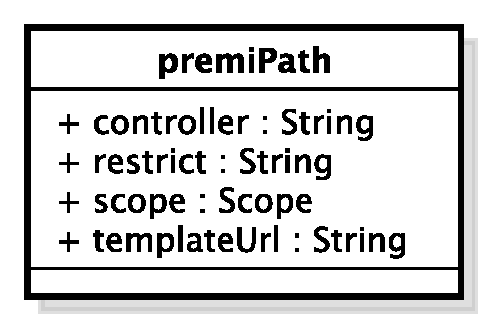
\includegraphics[scale=0.4,keepaspectratio]{diagrammi/classi/{frontEnd/directives/premiPath}.pdf}}
\caption{\nogloxy{Premi::Front-End::Directives::premiPath}}
\end{figure}
\FloatBarrier
\begin{itemize}
\item \textbf{Descrizione}\\
Rappresenta il componente grafico che permette all’utente di modificare il \gloxy{percorso} selezionato: togliendo dei nodi oppure rinominandolo.
Questo componente visualizza la lista dei nodi presenti nel \gloxy{percorso}. Per ogni nodo viene visualizzato il titolo del nodo ed un pulsante che permette di rimuoverlo dal \gloxy{percorso}.
\item \textbf{Utilizzo}\\
Viene utilizzata per consentire all’utente di modificare i \gloxy{percorsi di presentazione} che ha creato.
\item \textbf{Relazioni con altre classi}:
\begin{itemize}
\item \textit{IN} \hyperref[\nogloxy{Premi::Front-End::Controllers::PathController}]{\nogloxy{\texttt{PathController}}}\\
Classe che gestisce la visibilità e la logica della directive \texttt{premiPath}.
\item \textit{IN} \hyperref[\nogloxy{Premi::Front-End::Views::PathsEditorView}]{\nogloxy{\texttt{PathsEditorView}}}\\
\gloxy{View} dell’applicazione contenente la mappa mentale. Offre funzionalità legate ai \gloxy{percorsi} di presentazione.
Da questa \gloxy{view} è possibile:
\begin{itemize}
\item Creare/eliminare un \gloxy{percorso} di presentazione;
\item Modificare un \gloxy{percorso} aggiungendo e togliendo nodi, oppure rinominandolo;
\item Scegliere un \gloxy{percorso} da presentare e successivamente presentarlo.
\end{itemize}
\item \textit{OUT} \hyperref[\nogloxy{Premi::Front-End::Model::NodeReference}]{\nogloxy{\texttt{NodeReference}}}\\
Rappresenta il riferimento ad un nodo della mappa mentale, contiene l'identificativo e il titolo del del nodo.
\item \textit{OUT} \hyperref[\nogloxy{Premi::Front-End::Model::Path}]{\nogloxy{\texttt{Path}}}\\
Rappresenta un \gloxy{percorso di presentazione} costituito da una sequenza ordinata di passi.
\end{itemize}
\item \textbf{Attributi}:
\begin{itemize}
\item \nogloxy{\texttt{+ controller: String}}
\\ \dpDirectiveController
\item \nogloxy{\texttt{+ restrict: String}}
\\ \dpRestrict
\item \nogloxy{\texttt{+ scope: Scope}}
\\ \dpIsolatedScope \\
Lo scope deve contenere i seguenti oggetti:
\begin{itemize}
\item \texttt{selectedPath (=)}: oggetto \texttt{Path} da visualizzare e modificare;
\item \texttt{deselectPath (\&)}: funzione da invocare quando viene nascosta la directive.
\end{itemize}
\item \nogloxy{\texttt{+ templateUrl: String}}
\\ \dpTemplateUrl
\end{itemize}
\end{itemize}
\subsubsubsection{\nogloxy{Premi::Front-End::Directives::premiPathsList}}
\label{\nogloxy{Premi::Front-End::Directives::premiPathsList}}
\begin{figure}[h]
\centering
\nogloxy{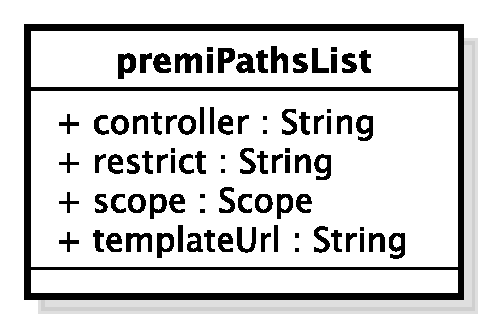
\includegraphics[scale=0.4,keepaspectratio]{diagrammi/classi/{frontEnd/directives/premiPathsList}.pdf}}
\caption{\nogloxy{Premi::Front-End::Directives::premiPathsList}}
\end{figure}
\FloatBarrier
\begin{itemize}
\item \textbf{Descrizione}\\
Rappresenta il componente grafico che si occupa di visualizzare la lista dei \gloxy{percorsi di presentazione} presenti nel \gloxy{progetto} corrente. Dalla lista dei \gloxy{percorsi} l'utente può selezionare un \gloxy{percorso} per modificarlo, cancellare un determinato \gloxy{percorso} oppure avviare la presentazione di quel \gloxy{percorso}. Questo componente contiene anche un pulsante per creare un nuovo \gloxy{progetto}.
\item \textbf{Utilizzo}\\
Viene utilizzata per mostrare all’utente i \gloxy{percorsi} già definiti nel \gloxy{progetto} corrente e per creare un \gloxy{percorso} vuoto.
\item \textbf{Relazioni con altre classi}:
\begin{itemize}
\item \textit{IN} \hyperref[\nogloxy{Premi::Front-End::Controllers::PathsListController}]{\nogloxy{\texttt{PathsListController}}}\\
Classe che gestisce le operazioni e la logica applicativa della directive \texttt{premiPathsList}.
\item \textit{IN} \hyperref[\nogloxy{Premi::Front-End::Views::PathsEditorView}]{\nogloxy{\texttt{PathsEditorView}}}\\
\gloxy{View} dell’applicazione contenente la mappa mentale. Offre funzionalità legate ai \gloxy{percorsi} di presentazione.
Da questa \gloxy{view} è possibile:
\begin{itemize}
\item Creare/eliminare un \gloxy{percorso} di presentazione;
\item Modificare un \gloxy{percorso} aggiungendo e togliendo nodi, oppure rinominandolo;
\item Scegliere un \gloxy{percorso} da presentare e successivamente presentarlo.
\end{itemize}
\end{itemize}
\item \textbf{Attributi}:
\begin{itemize}
\item \nogloxy{\texttt{+ controller: String}}
\\ \dpDirectiveController
\item \nogloxy{\texttt{+ restrict: String}}
\\ \dpRestrict
\item \nogloxy{\texttt{+ scope: Scope}}
\\ \dpIsolatedScope \\
Lo scope dovrà contenere i seguenti oggetti:
\begin{itemize}
\item \texttt{paths (=)}: \texttt{Array} contenente oggetti definiti con il \gloxy{JSON} ricevuto in risposta dalle \gloxy{API} del \gloxy{server}, in particolare questi oggetti hanno i seguenti campi dati: \texttt{$\_$id}, \texttt{name} e \texttt{default};
\item \texttt{selectPath (\&)} funzione da invocare quando l'utente preme il pulsante di modifica su un \gloxy{percorso} presente in lista.
\end{itemize}
\item \nogloxy{\texttt{+ templateUrl: String}}
\\ \dpTemplateUrl
\end{itemize}
\end{itemize}
\subsubsubsection{\nogloxy{Premi::Front-End::Directives::premiPresentation}}
\label{\nogloxy{Premi::Front-End::Directives::premiPresentation}}
\begin{figure}[h]
\centering
\nogloxy{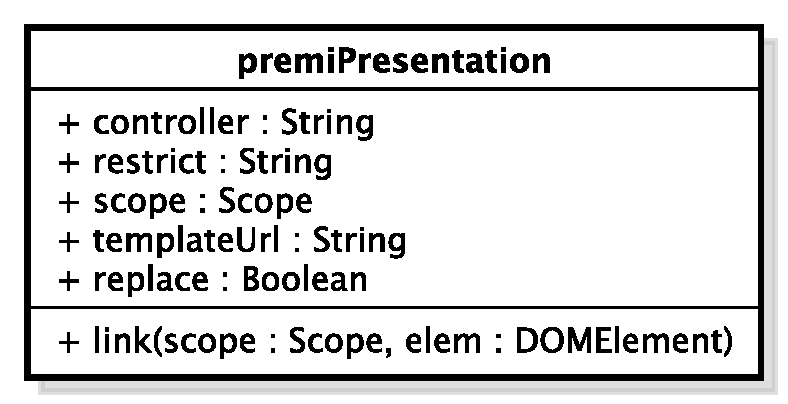
\includegraphics[scale=0.4,keepaspectratio]{diagrammi/classi/{frontEnd/directives/premiPresentation}.pdf}}
\caption{\nogloxy{Premi::Front-End::Directives::premiPresentation}}
\end{figure}
\FloatBarrier
\begin{itemize}
\item \textbf{Descrizione}\\
Rappresenta il componente grafico che genera la presentazione.
\item \textbf{Utilizzo}\\
Viene utilizzata per generare uno slideshow a partire dai nodi presenti nella mappa mentale.
\item \textbf{Relazioni con altre classi}:
\begin{itemize}
\item \textit{IN} \hyperref[\nogloxy{Premi::Front-End::Controllers::PresentationController}]{\nogloxy{\texttt{PresentationController}}}\\
Classe che si occupa di gestire la logica della presentazione di un \gloxy{percorso}. La gestione della presentazione funziona mediante l'emissione e l'ascolto di determinati eventi.
In particolare questa classe registra dei \textit{listeners} nell'oggetto \texttt{\$scope} per i seguenti eventi:
\begin{itemize}
\item \texttt{presentation-previousStep}: per tornare alla slide precedente;
\item \texttt{presentation-nextStep}: per passare alla slide successiva;
\item \texttt{presentation-goToId}: per passare alla slide contenente il nodo avente \texttt{id} uguale a quello associato all'evento;
\item \texttt{presentation-resumeLinear}: per riprendere la presentazione lineare dopo che si è verificato l'evento \texttt{presentation-goToId}.
\end{itemize}
Viene inoltre sollevato nello \texttt{\$scope} l'evento \texttt{presentation-goingToNode} con l'identificativo del nodo che sta per essere visualizzato ogni volta che si verifica un cambio slide.
\item \textit{IN} \hyperref[\nogloxy{Premi::Front-End::Views::PresentationView}]{\nogloxy{\texttt{PresentationView}}}\\
\gloxy{View} dell’applicazione che permette di effettuare la presentazione di un \gloxy{percorso} scelto dall’utente. Utilizza la directive \texttt{premiPresentation} per offrire funzionalità legate alla presentazione lineare e due menù per permettere all'utente di spostarsi in modo non lineare, seguendo le relazioni definite tra i nodi della mappa mentale.
Da questa vista è inoltre possibile stampare ed esportare il \gloxy{percorso di presentazione} in esecuzione, mediante le funzionalità offerte dal \gloxy{browser}.
\end{itemize}
\item \textbf{Attributi}:
\begin{itemize}
\item \nogloxy{\texttt{+ controller: String}}
\\ \dpDirectiveController
\item \nogloxy{\texttt{+ replace: Boolean}}
\\ \dpReplace
\item \nogloxy{\texttt{+ restrict: String}}
\\ \dpRestrict
\item \nogloxy{\texttt{+ scope: Scope}}
\\ \dpIsolatedScope \\
Lo scope deve contenere i seguenti oggetti:
\begin{itemize}
\item \texttt{paths (=)}: oggetto di tipo \texttt{Path} contenente le informazioni riguardanti il \gloxy{percorso} che si vuole presentare;
\item \texttt{nodes (=)}: \texttt{Array} contenente gli oggetti di tipo \texttt{PresentationNode} con i quali generare la presentazione;
\item \texttt{nodesIndex (=)}: oggetto contenente le informazioni riguardante la posizione dei nodi nella sequenza della presentazione. Le informazioni all'interno dell'oggetto sono memorizzate come coppie chiave/valore, usando come chiave l'id del nodo e come valore un \texttt{Array} contenente tutte le posizioni dell'array \texttt{nodes} in cui compare quel determinato nodo.
\end{itemize}
\item \nogloxy{\texttt{+ templateUrl: String}}
\\ \dpTemplateUrl
\end{itemize}
\item \textbf{Metodi}:
\begin{itemize}
\item \nogloxy{\texttt{+ link(scope: Scope, elem: DOMElement)}}
\\ \dpLinkFn \\ Viene utilizzata per integrare le funzionalità di Impress con \gloxy{Angular}.
\\ \textbf{Parametri}:
\begin{itemize}
\item \nogloxy{\texttt{scope: Scope}}
\\ Parametro contenente un riferimento allo \texttt{scope} della directive.
\item \nogloxy{\texttt{elem: DOMElement}}
\\ Parametro contenente un oggetto della \gloxy{libreria} \textit{jQuery} che rappresenta l'elemento del DOM associato alla directive.
\end{itemize}
\end{itemize}
\end{itemize}
\subsubsubsection{\nogloxy{Premi::Front-End::Directives::premiProjectSettingsEditor}}
\label{\nogloxy{Premi::Front-End::Directives::premiProjectSettingsEditor}}
\begin{figure}[h]
\centering
\nogloxy{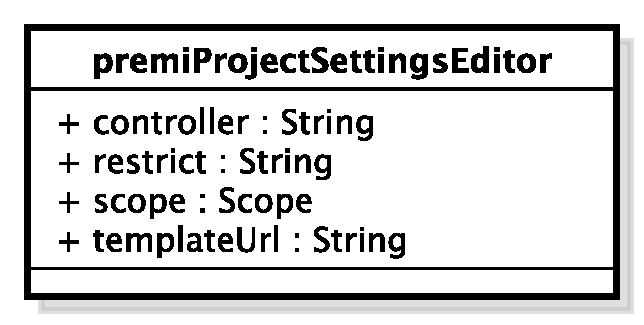
\includegraphics[scale=0.4,keepaspectratio]{diagrammi/classi/{frontEnd/directives/premiProjectSettingsEditor}.pdf}}
\caption{\nogloxy{Premi::Front-End::Directives::premiProjectSettingsEditor}}
\end{figure}
\FloatBarrier
\begin{itemize}
\item \textbf{Descrizione}\\
Rappresenta il componente grafico che permette di modificare i dati del \gloxy{progetto} aperto.
Questo componente presenta i vari campi per interagire con i parametri del \gloxy{progetto} e due pulsanti che l'utente utilizza per confermare o annullare le modifiche.
\item \textbf{Utilizzo}\\
Fornisce all’utente i controlli necessari per modificare i parametri del \gloxy{progetto} correntemente aperto.
\item \textbf{Relazioni con altre classi}:
\begin{itemize}
\item \textit{IN} \hyperref[\nogloxy{Premi::Front-End::Controllers::ProjectSettingsEditorController}]{\nogloxy{\texttt{ProjectSettingsEditorController}}}\\
Classe che si occupa di gestire la logica di funzionamento della directive \texttt{premiProjectSettingsEditor}.
\item \textit{IN} \hyperref[\nogloxy{Premi::Front-End::Directives::premiHeader}]{\nogloxy{\texttt{premiHeader}}}\\
Rappresenta la barra di navigazione che permette all’utente di spostarsi tra le varie views dell'applicazione. Fornisce inoltre i pulsanti per visualizzare il manuale utente, effettuare il logout, chiudere al presentazione e il \gloxy{progetto}. Inoltre, quando l'utente si trova nelle views in cui è possibile modificare il \gloxy{progetto}, questa directive permette di mostrare la finestra di modifica delle impostazioni del \gloxy{progetto}, sia di interagire con la visualizzazione della mappa mentale, modificando lo zoom e permettendo anche di stamparla.
\item \textit{OUT} \hyperref[\nogloxy{Premi::Front-End::Model::Project}]{\nogloxy{\texttt{Project}}}\\
Rappresenta un \gloxy{progetto} creato dall’utente. Contiene le informazioni riguardanti i parametri globali del \gloxy{progetto}: nome, formato del testo, colore di sfondo.
\end{itemize}
\item \textbf{Attributi}:
\begin{itemize}
\item \nogloxy{\texttt{+ controller: String}}
\\ \dpDirectiveController
\item \nogloxy{\texttt{+ restrict: String}}
\\ \dpRestrict
\item \nogloxy{\texttt{+ scope: Scope}}
\\ \dpIsolatedScope
\item \nogloxy{\texttt{+ templateUrl: String}}
\\ \dpTemplateUrl
\end{itemize}
\end{itemize}
\subsubsubsection{\nogloxy{Premi::Front-End::Directives::premiProjectsList}}
\label{\nogloxy{Premi::Front-End::Directives::premiProjectsList}}
\begin{figure}[h]
\centering
\nogloxy{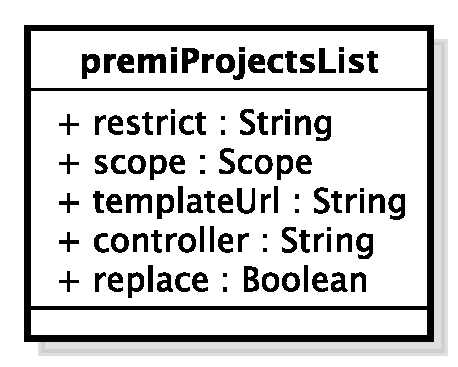
\includegraphics[scale=0.4,keepaspectratio]{diagrammi/classi/{frontEnd/directives/premiProjectsList}.pdf}}
\caption{\nogloxy{Premi::Front-End::Directives::premiProjectsList}}
\end{figure}
\FloatBarrier
\begin{itemize}
\item \textbf{Descrizione}\\
Rappresenta il componente grafico che mostra la lista dei \gloxy{progetti} creati dall’utente. Per ogni \gloxy{progetto} della lista è presente un pulsante che permette di modificarlo, di cancellarlo e di presentarlo.
\item \textbf{Utilizzo}\\
Viene utilizzata per permettere all’utente di interagire con i \gloxy{progetti} che ha creato.
\item \textbf{Relazioni con altre classi}:
\begin{itemize}
\item \textit{IN} \hyperref[\nogloxy{Premi::Front-End::Controllers::ProjectsListController}]{\nogloxy{\texttt{ProjectsListController}}}\\
Classe che gestisce la logica di funzionamento della directive \texttt{premiProjectsList}.
\item \textit{IN} \hyperref[\nogloxy{Premi::Front-End::Views::DashboardView}]{\nogloxy{\texttt{DashboardView}}}\\
\gloxy{View} dell’applicazione contenente la lista dei \gloxy{progetti} dell’utente correntemente autenticato.
Da questa \gloxy{view} è possibile:
\begin{itemize}
\item Creare un nuovo \gloxy{progetto};
\item Aprire un \gloxy{progetto} esistente per modificarlo oppure presentarlo;
\item Cancellare un \gloxy{progetto} esistente.
\end{itemize}
\item \textit{OUT} \hyperref[\nogloxy{Premi::Front-End::Model::Project}]{\nogloxy{\texttt{Project}}}\\
Rappresenta un \gloxy{progetto} creato dall’utente. Contiene le informazioni riguardanti i parametri globali del \gloxy{progetto}: nome, formato del testo, colore di sfondo.
\end{itemize}
\item \textbf{Attributi}:
\begin{itemize}
\item \nogloxy{\texttt{+ controller: String}}
\\ \dpDirectiveController
\item \nogloxy{\texttt{+ replace: Boolean}}
\\ \dpReplace
\item \nogloxy{\texttt{+ restrict: String}}
\\ \dpRestrict
\item \nogloxy{\texttt{+ scope: Scope}}
\\ \dpIsolatedScope \\
Lo scope deve contenere i seguenti oggetti:
\begin{itemize}
\item \texttt{projects (=)}: array contenente i \gloxy{progetti} da visualizzare;
\item \texttt{onEdit (\&)}: funzione da invocare quando l’utente seleziona un \gloxy{progetto} da aprire/modificare, la funzione viene invocata con un parametro corrispondente all’id del \gloxy{progetto};
\item \texttt{onDelete (\&)}: funzione da invocare quando l’utente seleziona un \gloxy{progetto} da eliminare, la funzione viene invocata con un parametro corrispondente all’id del \gloxy{progetto};
\item \texttt{onPlay (\&)}: funzione da invocare quando l’utente ha scelto un \gloxy{percorso di presentazione} da eseguire, la funzione viene invocata con due parametri di tipo stringa, il primo rappresentante l'id del \gloxy{progetto} e il secondo rappresentante l'id del \gloxy{percorso} da presentare.
\end{itemize}
\item \nogloxy{\texttt{+ templateUrl: String}}
\\ \dpTemplateUrl
\end{itemize}
\end{itemize}
\subsubsubsection{\nogloxy{Premi::Front-End::Directives::premiSmartMenu}}
\label{\nogloxy{Premi::Front-End::Directives::premiSmartMenu}}
\begin{figure}[h]
\centering
\nogloxy{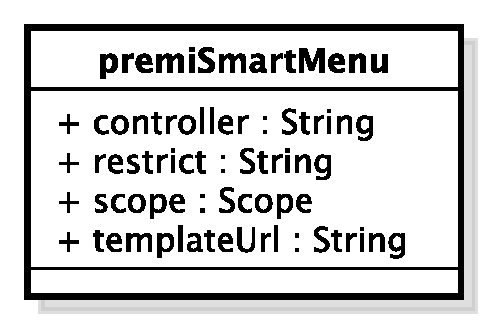
\includegraphics[scale=0.4,keepaspectratio]{diagrammi/classi/{frontEnd/directives/premiSmartMenu}.pdf}}
\caption{\nogloxy{Premi::Front-End::Directives::premiSmartMenu}}
\end{figure}
\FloatBarrier
\begin{itemize}
\item \textbf{Descrizione}\\
Rappresenta il menù che durante la presentazione permette di navigare la \gloxy{mappa mentale} seguendo le associazioni definite tra i vari nodi.
Questo componente consiste in una lista di elementi selezionabili dall’utente, ogni elemento corrisponde ad un'associazione presente tra il nodo corrente ed un altro nodo della mappa.
\item \textbf{Utilizzo}\\
Viene utilizzata per permettere all'utente di spostarsi tra i nodi della \gloxy{mappa mentale} seguendo le assocazioni presenti.
\item \textbf{Relazioni con altre classi}:
\begin{itemize}
\item \textit{IN} \hyperref[\nogloxy{Premi::Front-End::Controllers::SmartMenuController}]{\nogloxy{\texttt{SmartMenuController}}}\\
Classe che gestisce la visibilità della directive \texttt{premiSmartMenu}.
\item \textit{IN} \hyperref[\nogloxy{Premi::Front-End::Views::PresentationView}]{\nogloxy{\texttt{PresentationView}}}\\
\gloxy{View} dell’applicazione che permette di effettuare la presentazione di un \gloxy{percorso} scelto dall’utente. Utilizza la directive \texttt{premiPresentation} per offrire funzionalità legate alla presentazione lineare e due menù per permettere all'utente di spostarsi in modo non lineare, seguendo le relazioni definite tra i nodi della mappa mentale.
Da questa vista è inoltre possibile stampare ed esportare il \gloxy{percorso di presentazione} in esecuzione, mediante le funzionalità offerte dal \gloxy{browser}.
\item \textit{OUT} \hyperref[\nogloxy{Premi::Front-End::Model::NodeReference}]{\nogloxy{\texttt{NodeReference}}}\\
Rappresenta il riferimento ad un nodo della mappa mentale, contiene l'identificativo e il titolo del del nodo.
\end{itemize}
\item \textbf{Attributi}:
\begin{itemize}
\item \nogloxy{\texttt{+ controller: String}}
\\ \dpDirectiveController
\item \nogloxy{\texttt{+ restrict: String}}
\\ \dpRestrict
\item \nogloxy{\texttt{+ scope: Scope}}
\\ \dpIsolatedScope \\
Lo scope deve contenere i seguenti oggetti:
\begin{itemize}
\item \texttt{relations (=)}: \texttt{Array} contenente oggetti di tipo \texttt{NodeReference}, rappresentanti le associazioni che coinvolgono il nodo correntemente visualizzato;
\item \texttt{onClick (\&)}: funzione da invocare quando l’utente clicca su un elemento del menù. La funzione viene invocata con un parametro corrispondete all’id del nodo che compare nella relazione selezionata dall’utente.
\end{itemize}
\item \nogloxy{\texttt{+ templateUrl: String}}
\\ \dpTemplateUrl
\end{itemize}
\end{itemize}
\subsection{\nogloxy{Premi::Front-End::Model}}
\label{\nogloxy{Premi::Front-End::Model}}
\subsubsection{Informazioni generali}
\begin{figure}[h]
\centering
\nogloxy{\includegraphics[scale=0.4,keepaspectratio]{diagrammi/package/{frontEnd-model}.pdf}}
\caption{\nogloxy{Premi::Front-End::Model}}
\end{figure}
\FloatBarrier
\begin{itemize}
\item \textbf{Descrizione}\\
Package contenente le classi che definiscono la \gloxy{business logic} dell’applicazione.
\item \textbf{Padre}: \hyperref[\nogloxy{Premi::Front-End}]{\nogloxy{\texttt{Front-End}}}
\item \textbf{Interazioni con altri componenti}:
\begin{itemize}
\item \hyperref[\nogloxy{Premi::Front-End::Controllers}]{\nogloxy{\texttt{Controllers}}}\\
Package contenente i \gloxy{controller} della componente \gloxy{front-end} dell’applicazione.
\item \hyperref[\nogloxy{Premi::Front-End::Directives}]{\nogloxy{\texttt{Directives}}}\\
Package contenente le directives che compongno le views.
\item \hyperref[\nogloxy{Premi::Front-End::Services}]{\nogloxy{\texttt{Services}}}\\
Package contenente le classi che descrivono il meccanismo con cui il \gloxy{front-end} può interfacciarsi con le \gloxy{API} \gloxy{REST} del \gloxy{back-end}. Permette di popolare il model del \gloxy{client} e di richiedere l'esecuzione di operazioni al \gloxy{server}.
\item \hyperref[\nogloxy{Premi::Front-End::Views}]{\nogloxy{\texttt{Views}}}\\
Package contenente le views della componente \gloxy{front-end} dell’applicazione.
\end{itemize}
\end{itemize}
\subsubsection{Classi}
\subsubsubsection{\nogloxy{Premi::Front-End::Model::ErrorInfo}}
\label{\nogloxy{Premi::Front-End::Model::ErrorInfo}}
\begin{figure}[h]
\centering
\nogloxy{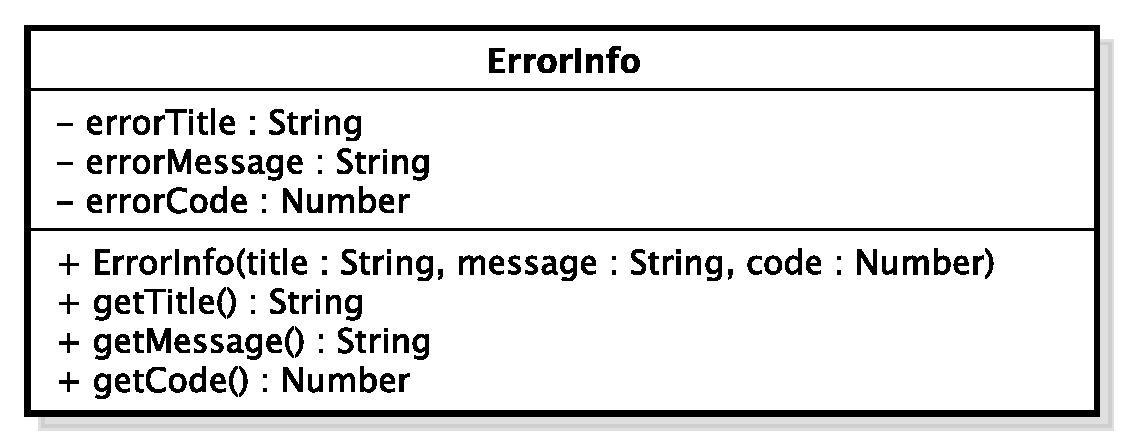
\includegraphics[scale=0.4,keepaspectratio]{diagrammi/classi/{frontEnd/model/ErrorInfo}.pdf}}
\caption{\nogloxy{Premi::Front-End::Model::ErrorInfo}}
\end{figure}
\FloatBarrier
\begin{itemize}
\item \textbf{Descrizione}\\
Rappresenta le informazioni di un errore che si è verificato eseguendo una determinata operazione.
\item \textbf{Utilizzo}\\
Viene utilizzata per racchiudere tutte le informazioni riguardanti l'errore.
\item \textbf{Relazioni con altre classi}:
\begin{itemize}
\item \textit{IN} \hyperref[\nogloxy{Premi::Front-End::AppRun}]{\nogloxy{\texttt{AppRun}}}\\
Classe che si occupa di gestire l'inizializzazione dell'applicazione.
\item \textit{IN} \hyperref[\nogloxy{Premi::Front-End::Directives::premiErrorMessage}]{\nogloxy{\texttt{premiErrorMessage}}}\\
Rappresenta il componente grafico che permette di mostrare messaggi d’errore all’utente all’interno dell’applicazione. Questo componente fornisce anche un pulsante che permette di nascondere il messaggio.
\item \textit{IN} \hyperref[\nogloxy{Premi::Front-End::Services::AuthenticationService}]{\nogloxy{\texttt{AuthenticationService}}}\\
Questa classe si occupa di gestire il processo di autenticazione e di registrazione di un utente.
\item \textit{IN} \hyperref[\nogloxy{Premi::Front-End::Services::MindmapService}]{\nogloxy{\texttt{MindmapService}}}\\
Questa classe si occupa del recupero e della modifica delle informazioni relative ai nodi e alle associazione presenti nella \gloxy{mappa mentale} del \gloxy{progetto} corrente. Utilizza \texttt{\$http} per comunicare con il \gloxy{back-end} e \texttt{MindmapAdapterService} per memorizzare i dati in locale.
\item \textit{IN} \hyperref[\nogloxy{Premi::Front-End::Services::PathService}]{\nogloxy{\texttt{PathService}}}\\
Questa classe si occupa del recupero e della modifica delle informazioni relative ai \gloxy{percorsi di presentazione} relativi al \gloxy{progetto} corrente.
\item \textit{IN} \hyperref[\nogloxy{Premi::Front-End::Services::PresentationService}]{\nogloxy{\texttt{PresentationService}}}\\
Questa classe si occupa del recupero e della modifica delle informazioni relative alle presentazioni del \gloxy{progetto} corrente.
\item \textit{IN} \hyperref[\nogloxy{Premi::Front-End::Services::ProjectService}]{\nogloxy{\texttt{ProjectService}}}\\
Questa classe si occupa del recupero e della modifica delle informazioni riguardanti i \gloxy{progetti}.
\end{itemize}
\item \textbf{Attributi}:
\begin{itemize}
\item \nogloxy{\texttt{- errorCode: Number}}
\\ Campo dati che contiene il codice dell'errore che si è verificato.
\item \nogloxy{\texttt{- errorMessage: String}}
\\ Campo dati contenente la descrizione dell'errore.
\item \nogloxy{\texttt{- errorTitle: String}}
\\ Campo dati che rappresenta il titolo del messaggio d'errore.
\end{itemize}
\item \textbf{Metodi}:
\begin{itemize}
\item \nogloxy{\texttt{+ ErrorInfo(title: String, message: String, code: Number)}}
\\ \dpConstructor
\\ \textbf{Parametri}:
\begin{itemize}
\item \nogloxy{\texttt{title: String}}
\\ Parametro contenente il titolo del messaggio d'errore.
\item \nogloxy{\texttt{message: String}}
\\ Parametro contenente al descrizione del messaggio d'errore.
\item \nogloxy{\texttt{code: Number}}
\\ Parametro contenente il codice del messaggio d'errore.
\end{itemize}
\item \nogloxy{\texttt{+ getCode(): Number}}
\\ Metodo \textit{getter} per il campo dati \texttt{errorCode}.
\item \nogloxy{\texttt{+ getMessage(): String}}
\\ Metodo \textit{getter} per il campo dati \texttt{errorMessage}.
\item \nogloxy{\texttt{+ getTitle(): String}}
\\ Metodo \textit{getter} per il campo dati \texttt{errorTitle}.
\end{itemize}
\end{itemize}
\subsubsubsection{\nogloxy{Premi::Front-End::Model::Node}}
\label{\nogloxy{Premi::Front-End::Model::Node}}
\begin{figure}[h]
\centering
\nogloxy{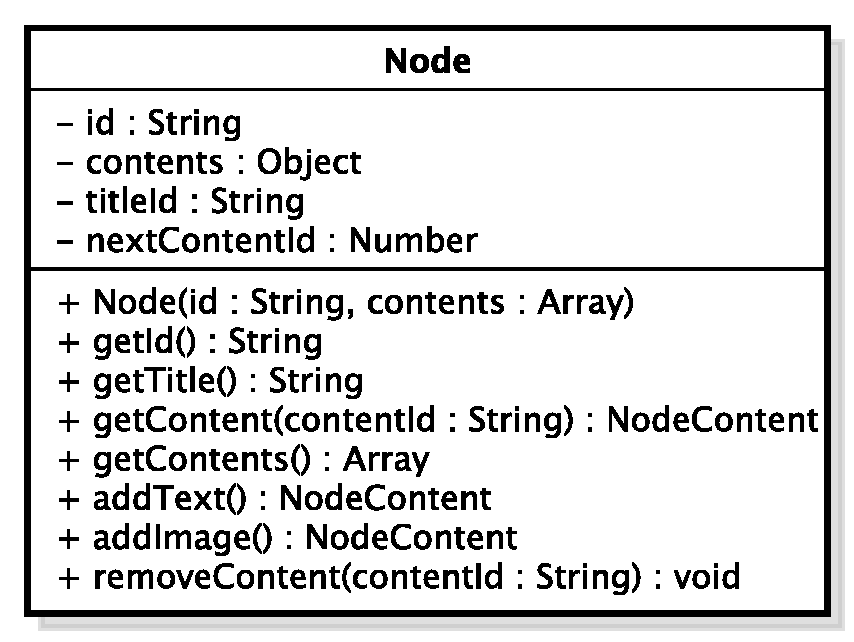
\includegraphics[scale=0.4,keepaspectratio]{diagrammi/classi/{frontEnd/model/Node}.pdf}}
\caption{\nogloxy{Premi::Front-End::Model::Node}}
\end{figure}
\FloatBarrier
\begin{itemize}
\item \textbf{Descrizione}\\
Rappresenta un nodo della mappa mentale. Contiene tutte le informazioni necessarie alla presentazione del contenuto del nodo.
\item \textbf{Utilizzo}\\
Viene utilizzata per memorizzare i dati di un nodo.
\item \textbf{Sottoclassi}:
\begin{itemize}
\item \hyperref[\nogloxy{Premi::Front-End::Model::PresentationNode}]{\nogloxy{\texttt{PresentationNode}}}
\end{itemize}
\item \textbf{Relazioni con altre classi}:
\begin{itemize}
\item \textit{IN} \hyperref[\nogloxy{Premi::Front-End::Controllers::ContextMenuController}]{\nogloxy{\texttt{ContextMenuController}}}\\
Classe che gestisce il comportamento della directive \texttt{premiContextMenu}.
\item \textit{IN} \hyperref[\nogloxy{Premi::Front-End::Controllers::MindmapEditorController}]{\nogloxy{\texttt{MindmapEditorController}}}\\
Classe che gestisce le operazioni e la logica applicativa riguardante la modifica di una mappa.
\item \textit{IN} \hyperref[\nogloxy{Premi::Front-End::Controllers::NodeContentsEditorController}]{\nogloxy{\texttt{NodeContentsEditorController}}}\\
Classe che si occupa di gestire la logica legata alla modifica del contenuto di un nodo.
\item \textit{IN} \hyperref[\nogloxy{Premi::Front-End::Controllers::NodeController}]{\nogloxy{\texttt{NodeController}}}\\
Classe che si occupa di gestire il funzionamento della directive \texttt{premiNode}.
\item \textit{IN} \hyperref[\nogloxy{Premi::Front-End::Controllers::PathsEditorController}]{\nogloxy{\texttt{PathsEditorController}}}\\
Classe che gestisce le operazioni e la logica applicativa riguardante la gestione dei \gloxy{percorsi di presentazione} definiti sulla mappa mentale.
\item \textit{IN} \hyperref[\nogloxy{Premi::Front-End::Controllers::PresentationViewerController}]{\nogloxy{\texttt{PresentationViewerController}}}\\
Classe che gestisce le operazioni e la logica applicativa riguardante l’esecuzione di un \gloxy{percorso} di presentazione.
\item \textit{IN} \hyperref[\nogloxy{Premi::Front-End::Directives::premiAddToPath}]{\nogloxy{\texttt{premiAddToPath}}}\\
Rappresenta il componente grafico che permette all’utente di visualizzare il contenuto di un nodo e di aggiungerlo ad uno dei \gloxy{percorsi di presentazione} esistenti.
Questo componente visualizza una lista contenente tutti i \gloxy{percorsi} disponibili al quale, selezionando quello desiderato, è possibile aggiungere il nodo slezionato.
\item \textit{IN} \hyperref[\nogloxy{Premi::Front-End::Directives::premiNode}]{\nogloxy{\texttt{premiNode}}}\\
Rappresenta il componente grafico che visualizza il contenuto di un nodo. Questo contenuto non deve essere modificabile.
\item \textit{IN} \hyperref[\nogloxy{Premi::Front-End::Directives::premiNodeContentsEditor}]{\nogloxy{\texttt{premiNodeContentsEditor}}}\\
Rappresenta il componente grafico che permette all’utente di modificare il contenuto di un nodo. Questo componente fornisce all’utente sia dei campi per inserire/modificare il contenuto del nodo, sia un’anteprima di come questo verrà visualizzato. Dall’anteprima sarà anche possibile spostare e ridimensionare i vari componenti.
Saranno presenti inoltre due pulsanti, uno per confermare le modifiche e l’altro per annullarle e ripristinare lo stato del nodo.
\item \textit{IN} \hyperref[\nogloxy{Premi::Front-End::Services::MindmapService}]{\nogloxy{\texttt{MindmapService}}}\\
Questa classe si occupa del recupero e della modifica delle informazioni relative ai nodi e alle associazione presenti nella \gloxy{mappa mentale} del \gloxy{progetto} corrente. Utilizza \texttt{\$http} per comunicare con il \gloxy{back-end} e \texttt{MindmapAdapterService} per memorizzare i dati in locale.
\item \textit{IN} \hyperref[\nogloxy{Premi::Front-End::Views::MindmapEditorView}]{\nogloxy{\texttt{MindmapEditorView}}}\\
\gloxy{View} dell’applicazione contenente la mappa mentale. Offre funzionalità di modifica della mappa.
Da questa \gloxy{view} è possibile:
\begin{itemize}
\item Aggiungere/togliere nodi;
\item Modificare il contenuto di un nodo;
\item Aggiungere/togliere associazioni tra nodi;
\item Modificare i parametri del \gloxy{progetto}.
\end{itemize}
\item \textit{IN} \hyperref[\nogloxy{Premi::Front-End::Views::PathsEditorView}]{\nogloxy{\texttt{PathsEditorView}}}\\
\gloxy{View} dell’applicazione contenente la mappa mentale. Offre funzionalità legate ai \gloxy{percorsi} di presentazione.
Da questa \gloxy{view} è possibile:
\begin{itemize}
\item Creare/eliminare un \gloxy{percorso} di presentazione;
\item Modificare un \gloxy{percorso} aggiungendo e togliendo nodi, oppure rinominandolo;
\item Scegliere un \gloxy{percorso} da presentare e successivamente presentarlo.
\end{itemize}
\item \textit{OUT} \hyperref[\nogloxy{Premi::Front-End::Model::NodeContent}]{\nogloxy{\texttt{NodeContent}}}\\
Rappresenta il contenuto di un nodo. Contiene informazioni che indicano deve essere visualizzato il contenuto all’interno del nodo.
\end{itemize}
\item \textbf{Attributi}:
\begin{itemize}
\item \nogloxy{\texttt{- contents: Object}}
\\ Attributo che rappresenta i dati contenuti nel nodo, i vari oggetti \texttt{NodeContent} vengono memorizzati all'interno dell'oggetto come coppie chiave/valore, usando come chiavi gli \texttt{id} devi vari \texttt{NodeContent}.
\item \nogloxy{\texttt{- id: String}}
\\ Attributo che rappresenta l'identificativo del nodo.
\item \nogloxy{\texttt{- nextContentId: Number}}
\\ Campo dati contenente l'\texttt{id} da dare al prossimo contenuto che verrà aggiunto al nodo.
\item \nogloxy{\texttt{- titleId: String}}
\\ Attributo che rappresenta l'id del \texttt{NodeContent} presente nell'array \texttt{content} e che contiene il titolo del nodo.
\end{itemize}
\item \textbf{Metodi}:
\begin{itemize}
\item \nogloxy{\texttt{+ addImage(): NodeContent}}
\\ Metodo che aggiunge ai contenuti del nodo un'immagine utilizzando dei dati di default. Viene ritornato un riferimento all'oggetto creato.
\item \nogloxy{\texttt{+ addText(): NodeContent}}
\\ Metodo che aggiunge ai contenuti del nodo un elemento testuale utilizzando dei dati di default. Viene ritornato un riferimento all'oggetto creato.
\item \nogloxy{\texttt{+ getContent(contentId: String): NodeContent}}
\\ Metodo che ritorna l'oggetto di \texttt{NodeContent} presente all'interno del nodo avente \texttt{id} uguale a quello ricevuto come parametro.
\\ \textbf{Parametri}:
\begin{itemize}
\item \nogloxy{\texttt{contentId: String}}
\\ Parametro che rappresenta l'\texttt{id} dell'oggetto richiesto.
\end{itemize}
\item \nogloxy{\texttt{+ getContents(): Array}}
\\ Metodo che restituisce tutti gli oggetti \texttt{NodeContent} contenuti nel nodo.
\item \nogloxy{\texttt{+ getId(): String}}
\\ Metodo che ritorna l'\texttt{id} del nodo.
\item \nogloxy{\texttt{+ getTitle(): String}}
\\ Metodo che, uttilizza il campo dati \texttt{titleId} per recuperare dall'array \texttt{contents}, restituisce una stringa contenente il titolo del nodo.
\item \nogloxy{\texttt{+ Node(id: String, contents: Array)}}
\\ \dpConstructor
\\ \textbf{Parametri}:
\begin{itemize}
\item \nogloxy{\texttt{id: String}}
\\ Parametro che rappresenta l'\texttt{id} da dare al nuovo oggetto.
\item \nogloxy{\texttt{contents: Array}}
\\ Parametro che rappresenta i contenuti da inserire all'interno del nuovo nodo. L'array deve contenere almeno un \texttt{NodeContent} di tipo 'title'. All'interno dell'array gli oggetti possono essere di tipo \texttt{NodeContent} oppure essere definiti con il \texttt{\gloxy{JSON}} ricevuto in risposta dalle \gloxy{API} del \gloxy{back-end}.
\end{itemize}
\item \nogloxy{\texttt{+ removeContent(contentId: String): void}}
\\ Metodo che rimuove dalla collezione \texttt{content} l'elemento avente \texttt{id} uguale a \texttt{contentId}.
\\ \textbf{Parametri}:
\begin{itemize}
\item \nogloxy{\texttt{contentId: String}}
\\ Parametro che rappresenta l'\texttt{id} dell'oggetto \texttt{NodeContent} da rimuovere.
\end{itemize}
\end{itemize}
\end{itemize}
\subsubsubsection{\nogloxy{Premi::Front-End::Model::NodeContent}}
\label{\nogloxy{Premi::Front-End::Model::NodeContent}}
\begin{figure}[h]
\centering
\nogloxy{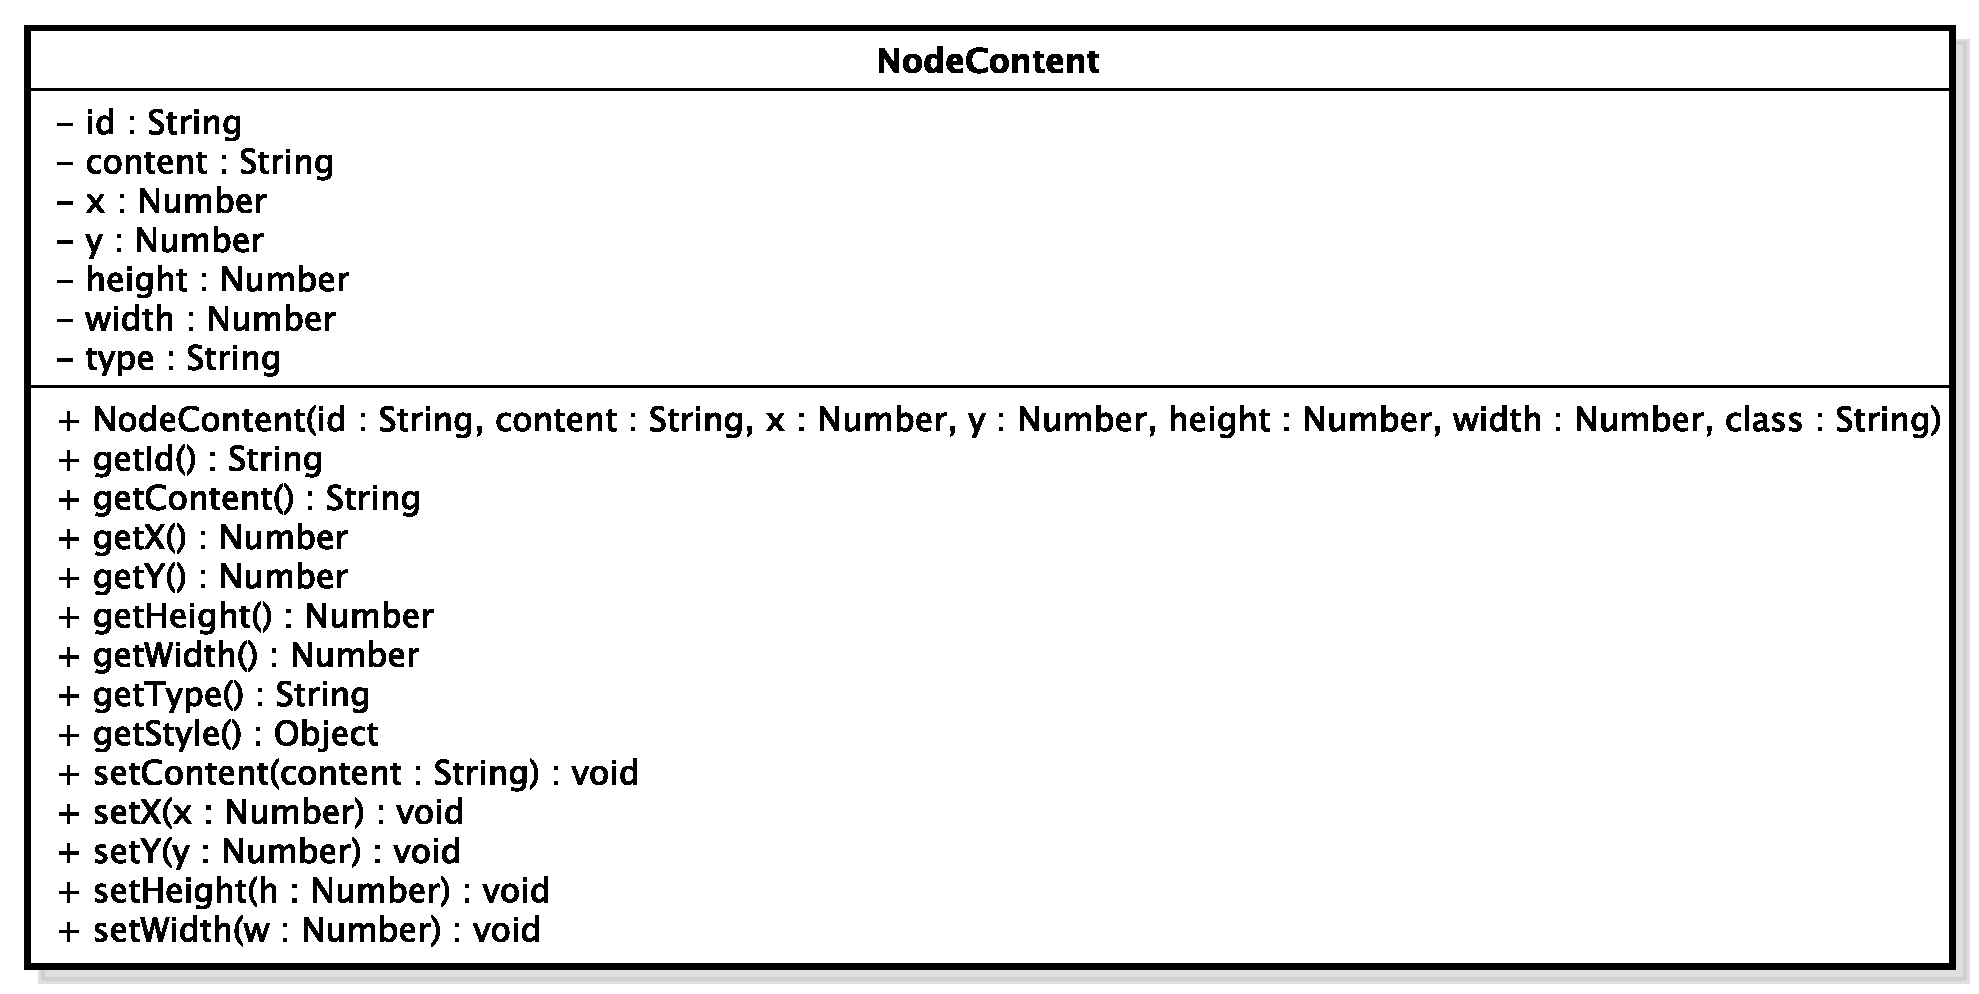
\includegraphics[scale=0.4,keepaspectratio]{diagrammi/classi/{frontEnd/model/NodeContent}.pdf}}
\caption{\nogloxy{Premi::Front-End::Model::NodeContent}}
\end{figure}
\FloatBarrier
\begin{itemize}
\item \textbf{Descrizione}\\
Rappresenta il contenuto di un nodo. Contiene informazioni che indicano deve essere visualizzato il contenuto all’interno del nodo.
\item \textbf{Utilizzo}\\
Viene utilizzata per memorizzare i vari oggetti che sono contenuti in un nodo.
\item \textbf{Relazioni con altre classi}:
\begin{itemize}
\item \textit{IN} \hyperref[\nogloxy{Premi::Front-End::Controllers::NodeContentsEditorController}]{\nogloxy{\texttt{NodeContentsEditorController}}}\\
Classe che si occupa di gestire la logica legata alla modifica del contenuto di un nodo.
\item \textit{IN} \hyperref[\nogloxy{Premi::Front-End::Directives::premiEditableNodeContent}]{\nogloxy{\texttt{premiEditableNodeContent}}}\\
Rappresenta un elemento contenuto nel \gloxy{frame} di un nodo. Questo elemento è spostabile e ridimensionabile. Le modifiche effettuate su questo elemento vengono riportate direttamente sull’oggetto \texttt{nodeContent}.
Questo componente deve essere in grado di rappresentare le varie tipologie di contenuto che possono essere presenti all’interno di un nodo. La discriminazione del tipo del contenuto deve essere fatta in base ai campi dati dell’oggetto \texttt{nodeContent}.
\item \textit{IN} \hyperref[\nogloxy{Premi::Front-End::Directives::premiNodeContent}]{\nogloxy{\texttt{premiNodeContent}}}\\
Rappresenta un elemento contenuto nel \gloxy{frame} di un nodo.
Questo componente deve essere in grado di rappresentare le varie tipologie di contenuto che possono essere presenti all’interno di un nodo.  La discriminazione del tipo del contenuto deve essere fatta in base ai campi dati dell’oggetto \texttt{nodeContent}.
\item \textit{IN} \hyperref[\nogloxy{Premi::Front-End::Model::Node}]{\nogloxy{\texttt{Node}}}\\
Rappresenta un nodo della mappa mentale. Contiene tutte le informazioni necessarie alla presentazione del contenuto del nodo.
\item \textit{IN} \hyperref[\nogloxy{Premi::Front-End::Model::PresentationNode}]{\nogloxy{\texttt{PresentationNode}}}\\
Classe che estende \texttt{Node}, riproducendo una struttura comoda per poter presentare i contenuti di un nodo e semplificare lo spostamento fra \gloxy{frame} associati e con relazioni di tipo gerarchico.
\end{itemize}
\item \textbf{Attributi}:
\begin{itemize}
\item \nogloxy{\texttt{- content: String}}
\\ Attributo che rappresenta i dati del contenuto del nodo.
\item \nogloxy{\texttt{- height: Number}}
\\ Attributo che rappresenta l'altezza del contenuto del nodo.
\item \nogloxy{\texttt{- id: String}}
\\ Attributo che rappresenta l'identificativo del contenuto.
\item \nogloxy{\texttt{- type: String}}
\\ Attributo che rappresenta il tipo di contenuto del nodo.
\item \nogloxy{\texttt{- width: Number}}
\\ Attributo che rappresenta la larghezza del contenuto del nodo.
\item \nogloxy{\texttt{- x: Number}}
\\ Attributo che rappresenta la posizione rispetto all'asse delle x del contenuto del nodo.
\item \nogloxy{\texttt{- y: Number}}
\\ Attributo che rappresenta la posizione rispetto all'asse delle y del contenuto del nodo.
\end{itemize}
\item \textbf{Metodi}:
\begin{itemize}
\item \nogloxy{\texttt{+ getContent(): String}}
\\ Metodo che restituisce il valore dell'attributo \texttt{content}.
\item \nogloxy{\texttt{+ getHeight(): Number}}
\\ Metodo che restituisce il valore dell'attributo \texttt{height}.
\item \nogloxy{\texttt{+ getId(): String}}
\\ Metodo che restituisce il valore dell'attributo \texttt{id}.
\item \nogloxy{\texttt{+ getStyle(): Object}}
\\ Metodo che restituisce un oggetto contenente le informazioni riguardanti lo stile \gloxy{CSS} del contenuto del nodo. L'oggetto conterrà i seguenti campi dati: \texttt{top}, \texttt{left}, \texttt{width}, \texttt{height} e \texttt{position}.
\item \nogloxy{\texttt{+ getType(): String}}
\\ Metodo che restituisce il valore dell'attributo \texttt{type}.
\item \nogloxy{\texttt{+ getWidth(): Number}}
\\ Metodo che restituisce il valore dell'attributo \texttt{width}.
\item \nogloxy{\texttt{+ getX(): Number}}
\\ Metodo che restituisce il valore dell'attributo \texttt{x}.
\item \nogloxy{\texttt{+ getY(): Number}}
\\ Metodo che restituisce il valore dell'attributo \texttt{Y}.
\item \nogloxy{\texttt{+ NodeContent(id: String, content: String, x: Number, y: Number, height: Number, width: Number, type: String)}}
\\ Costruttore di \texttt{NodeContent}. Crea un'istanza con contenuto, posizione rispetto all'asse delle x e delle y, altezza, larghezza e tipo di contenuto pari ai valori dei parametri \texttt{id}, \texttt{content}, \texttt{x}, \texttt{y}, \texttt{height}, \texttt{width} e \texttt{class}.
\\ \textbf{Parametri}:
\begin{itemize}
\item \nogloxy{\texttt{id: String}}
\\ Parametro che rappresenta l'\texttt{id} da dare all'oggetto.
\item \nogloxy{\texttt{content: String}}
\\ Parametro che rappresenta il contenuto dell'oggetto.
\item \nogloxy{\texttt{x: Number}}
\\ Parametro che rappresenta lo spostamento rispetto l'asse x dell'oggetto.
\item \nogloxy{\texttt{y: Number}}
\\ Parametro che rappresenta lo spostamento rispetto l'asse y dell'oggetto
\item \nogloxy{\texttt{height: Number}}
\\ Parametro che rappresenta l'altezza dell'oggetto.
\item \nogloxy{\texttt{width: Number}}
\\ Parametro che rappresenta la larghezza dell'oggetto.
\item \nogloxy{\texttt{type: String}}
\\ Parametro che rappresenta il tipo di contenuto presente nel campo \texttt{content} dell'oggetto.
\end{itemize}
\item \nogloxy{\texttt{+ setContent(content: String): void}}
\\ Metodo che imposta il valore del campo dati \texttt{content}.
\\ \textbf{Parametri}:
\begin{itemize}
\item \nogloxy{\texttt{content: String}}
\\ Parametro che rappresenta il valore da assegnare.
\end{itemize}
\item \nogloxy{\texttt{+ setHeight(h: Number): void}}
\\ Metodo che imposta il valore del campo dati \texttt{height}.
\\ \textbf{Parametri}:
\begin{itemize}
\item \nogloxy{\texttt{h: Number}}
\\ Parametro che rappresenta il valore da assegnare.
\end{itemize}
\item \nogloxy{\texttt{+ setWidth(w: Number): void}}
\\ Metodo che imposta il valore del campo dati \texttt{width}.
\\ \textbf{Parametri}:
\begin{itemize}
\item \nogloxy{\texttt{w: Number}}
\\ Parametro che rappresenta il valore da assegnare.
\end{itemize}
\item \nogloxy{\texttt{+ setX(x: Number): void}}
\\ Metodo che imposta il valore del campo dati \texttt{x}.
\\ \textbf{Parametri}:
\begin{itemize}
\item \nogloxy{\texttt{x: Number}}
\\ Parametro che rappresenta il valore da assegnare.
\end{itemize}
\item \nogloxy{\texttt{+ setY(y: Number): void}}
\\ Metodo che imposta il valore del campo dati \texttt{y}.
\\ \textbf{Parametri}:
\begin{itemize}
\item \nogloxy{\texttt{y: Number}}
\\ Parametro che rappresenta il valore da assegnare.
\end{itemize}
\end{itemize}
\end{itemize}
\subsubsubsection{\nogloxy{Premi::Front-End::Model::NodeReference}}
\label{\nogloxy{Premi::Front-End::Model::NodeReference}}
\begin{figure}[h]
\centering
\nogloxy{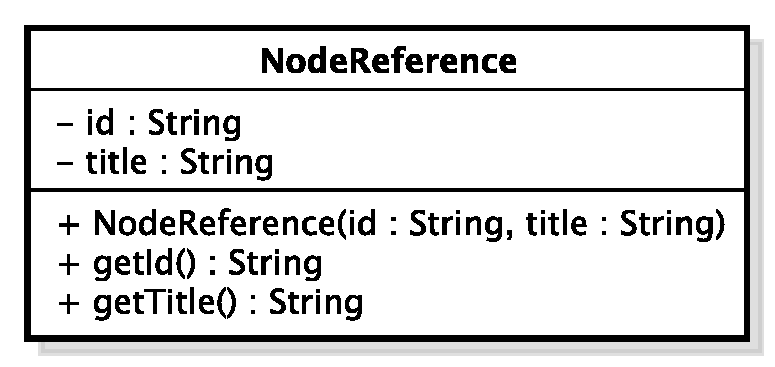
\includegraphics[scale=0.4,keepaspectratio]{diagrammi/classi/{frontEnd/model/NodeReference}.pdf}}
\caption{\nogloxy{Premi::Front-End::Model::NodeReference}}
\end{figure}
\FloatBarrier
\begin{itemize}
\item \textbf{Descrizione}\\
Rappresenta il riferimento ad un nodo della mappa mentale, contiene l'identificativo e il titolo del del nodo.
\item \textbf{Utilizzo}\\
Viene utilizzata per riferirsi ad un nodo della mappa mentale. Oggetti di questo tipo vengono usati per rappresentare sia i passi di un \gloxy{percorso} di presentazione, sia per i nodi in relazione con un oggetto di tipo \texttt{PresentationNode}.
\item \textbf{Relazioni con altre classi}:
\begin{itemize}
\item \textit{IN} \hyperref[\nogloxy{Premi::Front-End::Directives::premiHierarchicalMenu}]{\nogloxy{\texttt{premiHierarchicalMenu}}}\\
Rappresenta il menù che durante la presentazione permette di navigare la \gloxy{mappa mentale} seguendo le relazioni gerarchiche presenti tra i vari nodi della mappa mentale. Questo componente consiste in una lista di elementi selezionabili dall’utente, ogni elemento corrisponde ad una relazione presente tra il nodo corrente ed un altro nodo della mappa.
\item \textit{IN} \hyperref[\nogloxy{Premi::Front-End::Directives::premiPath}]{\nogloxy{\texttt{premiPath}}}\\
Rappresenta il componente grafico che permette all’utente di modificare il \gloxy{percorso} selezionato: togliendo dei nodi oppure rinominandolo.
Questo componente visualizza la lista dei nodi presenti nel \gloxy{percorso}. Per ogni nodo viene visualizzato il titolo del nodo ed un pulsante che permette di rimuoverlo dal \gloxy{percorso}.
\item \textit{IN} \hyperref[\nogloxy{Premi::Front-End::Directives::premiSmartMenu}]{\nogloxy{\texttt{premiSmartMenu}}}\\
Rappresenta il menù che durante la presentazione permette di navigare la \gloxy{mappa mentale} seguendo le associazioni definite tra i vari nodi.
Questo componente consiste in una lista di elementi selezionabili dall’utente, ogni elemento corrisponde ad un'associazione presente tra il nodo corrente ed un altro nodo della mappa.
\item \textit{IN} \hyperref[\nogloxy{Premi::Front-End::Model::Path}]{\nogloxy{\texttt{Path}}}\\
Rappresenta un \gloxy{percorso di presentazione} costituito da una sequenza ordinata di passi.
\item \textit{IN} \hyperref[\nogloxy{Premi::Front-End::Model::PresentationNode}]{\nogloxy{\texttt{PresentationNode}}}\\
Classe che estende \texttt{Node}, riproducendo una struttura comoda per poter presentare i contenuti di un nodo e semplificare lo spostamento fra \gloxy{frame} associati e con relazioni di tipo gerarchico.
\end{itemize}
\item \textbf{Attributi}:
\begin{itemize}
\item \nogloxy{\texttt{- id: String}}
\\ Attributo che rappresenta l'identificativo del nodo associato al passo di \gloxy{percorso} di presentazione.
\item \nogloxy{\texttt{- title: String}}
\\ Attributo che rappresenta il titolo del nodo nel passo del \gloxy{percorso} di presentazione.
\end{itemize}
\item \textbf{Metodi}:
\begin{itemize}
\item \nogloxy{\texttt{+ getId(): String}}
\\ Metodo che restituisce l'identificativo del nodo associato al passo di \gloxy{percorso} di presentazione.
\item \nogloxy{\texttt{+ getTitle(): String}}
\\ Metodo che restituisce il titolo del passo di \gloxy{percorso} di presentazione.
\item \nogloxy{\texttt{+ NodeReference(id: String, title: String)}}
\\ \dpConstructor
\\ \textbf{Parametri}:
\begin{itemize}
\item \nogloxy{\texttt{id: String}}
\\ Parametro che rappresenta l'\texttt{id} del nodo che compare in un \gloxy{percorso} di presentazione.
\item \nogloxy{\texttt{title: String}}
\\ Parametro che rappresenta il titolo del nodo che compare in un \gloxy{percorso} di presentazione.
\end{itemize}
\end{itemize}
\end{itemize}
\subsubsubsection{\nogloxy{Premi::Front-End::Model::Path}}
\label{\nogloxy{Premi::Front-End::Model::Path}}
\begin{figure}[h]
\centering
\nogloxy{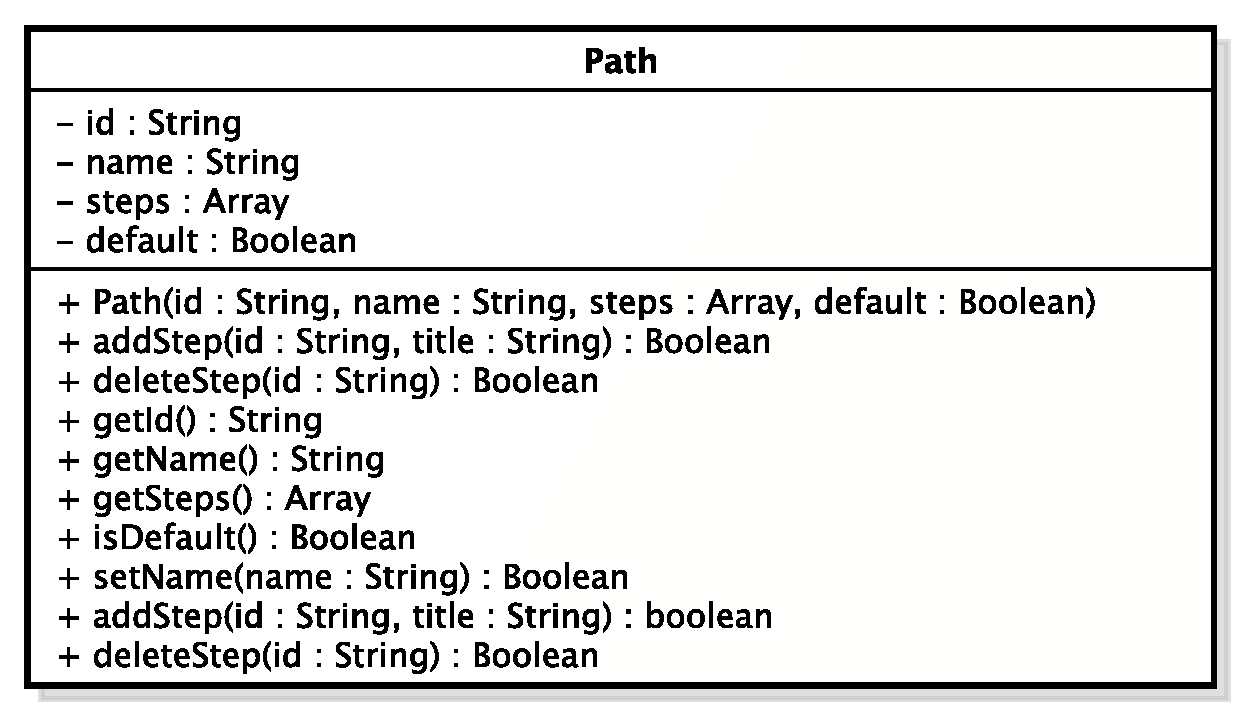
\includegraphics[scale=0.4,keepaspectratio]{diagrammi/classi/{frontEnd/model/Path}.pdf}}
\caption{\nogloxy{Premi::Front-End::Model::Path}}
\end{figure}
\FloatBarrier
\begin{itemize}
\item \textbf{Descrizione}\\
Rappresenta un \gloxy{percorso di presentazione} costituito da una sequenza ordinata di passi.
\item \textbf{Utilizzo}\\
Viene utilizzata per memorizzare un \gloxy{percorso} di presentazione.
\item \textbf{Relazioni con altre classi}:
\begin{itemize}
\item \textit{IN} \hyperref[\nogloxy{Premi::Front-End::Controllers::PathController}]{\nogloxy{\texttt{PathController}}}\\
Classe che gestisce la visibilità e la logica della directive \texttt{premiPath}.
\item \textit{IN} \hyperref[\nogloxy{Premi::Front-End::Controllers::PathsEditorController}]{\nogloxy{\texttt{PathsEditorController}}}\\
Classe che gestisce le operazioni e la logica applicativa riguardante la gestione dei \gloxy{percorsi di presentazione} definiti sulla mappa mentale.
\item \textit{IN} \hyperref[\nogloxy{Premi::Front-End::Controllers::PathsListController}]{\nogloxy{\texttt{PathsListController}}}\\
Classe che gestisce le operazioni e la logica applicativa della directive \texttt{premiPathsList}.
\item \textit{IN} \hyperref[\nogloxy{Premi::Front-End::Controllers::PresentationViewerController}]{\nogloxy{\texttt{PresentationViewerController}}}\\
Classe che gestisce le operazioni e la logica applicativa riguardante l’esecuzione di un \gloxy{percorso} di presentazione.
\item \textit{IN} \hyperref[\nogloxy{Premi::Front-End::Directives::premiPath}]{\nogloxy{\texttt{premiPath}}}\\
Rappresenta il componente grafico che permette all’utente di modificare il \gloxy{percorso} selezionato: togliendo dei nodi oppure rinominandolo.
Questo componente visualizza la lista dei nodi presenti nel \gloxy{percorso}. Per ogni nodo viene visualizzato il titolo del nodo ed un pulsante che permette di rimuoverlo dal \gloxy{percorso}.
\item \textit{IN} \hyperref[\nogloxy{Premi::Front-End::Services::PathService}]{\nogloxy{\texttt{PathService}}}\\
Questa classe si occupa del recupero e della modifica delle informazioni relative ai \gloxy{percorsi di presentazione} relativi al \gloxy{progetto} corrente.
\item \textit{IN} \hyperref[\nogloxy{Premi::Front-End::Views::PathsEditorView}]{\nogloxy{\texttt{PathsEditorView}}}\\
\gloxy{View} dell’applicazione contenente la mappa mentale. Offre funzionalità legate ai \gloxy{percorsi} di presentazione.
Da questa \gloxy{view} è possibile:
\begin{itemize}
\item Creare/eliminare un \gloxy{percorso} di presentazione;
\item Modificare un \gloxy{percorso} aggiungendo e togliendo nodi, oppure rinominandolo;
\item Scegliere un \gloxy{percorso} da presentare e successivamente presentarlo.
\end{itemize}
\item \textit{IN} \hyperref[\nogloxy{Premi::Front-End::Views::PresentationView}]{\nogloxy{\texttt{PresentationView}}}\\
\gloxy{View} dell’applicazione che permette di effettuare la presentazione di un \gloxy{percorso} scelto dall’utente. Utilizza la directive \texttt{premiPresentation} per offrire funzionalità legate alla presentazione lineare e due menù per permettere all'utente di spostarsi in modo non lineare, seguendo le relazioni definite tra i nodi della mappa mentale.
Da questa vista è inoltre possibile stampare ed esportare il \gloxy{percorso di presentazione} in esecuzione, mediante le funzionalità offerte dal \gloxy{browser}.
\item \textit{OUT} \hyperref[\nogloxy{Premi::Front-End::Model::NodeReference}]{\nogloxy{\texttt{NodeReference}}}\\
Rappresenta il riferimento ad un nodo della mappa mentale, contiene l'identificativo e il titolo del del nodo.
\end{itemize}
\item \textbf{Attributi}:
\begin{itemize}
\item \nogloxy{\texttt{- default: Boolean}}
\\ Campo dati che specifica se il \gloxy{percorso di presentazione} è quello di default.
\item \nogloxy{\texttt{- id: String}}
\\ Attributo che rappresenta l'identificativo del \gloxy{percorso} di presentazione.
\item \nogloxy{\texttt{- name: String}}
\\ Attributo che rappresenta il nome del \gloxy{percorso} di presentazione.
\item \nogloxy{\texttt{- steps: Array}}
\\ Attributo che rappresenta la successione dei passi del \gloxy{percorso} di presentazione.
\end{itemize}
\item \textbf{Metodi}:
\begin{itemize}
\item \nogloxy{\texttt{+ addStep(id: String, title: String): Boolean}}
\\ Metodo che inserisce il passo di presentazione, formato dai valori dei parametri \texttt{id} e \texttt{title}, rispettivamente, in coda alla successione dei passi del \gloxy{percorso} di presentazione.
\\ \textbf{Parametri}:
\begin{itemize}
\item \nogloxy{\texttt{id: String}}
\\ Parametro che rappresenta l'identificativo del nodo da associare al nuovo passo di \gloxy{percorso} di presentazione.
\item \nogloxy{\texttt{title: String}}
\\ Parametro che rappresenta il titolo del passo di \gloxy{percorso di presentazione} da aggiungere.
\end{itemize}
\item \nogloxy{\texttt{+ deleteStep(id: String): Boolean}}
\\ Metodo che rimuove l'ultimo passo del \gloxy{percorso di presentazione} con id pari al valore del parametro \texttt{id} e restituisce \texttt{true} se e solo se avviene tale rimozione.
\\ \textbf{Parametri}:
\begin{itemize}
\item \nogloxy{\texttt{id: String}}
\\ Parametro che rappresenta l'identificativo del nodo associato al passo di \gloxy{percorso di presentazione} da rimuovere.
\end{itemize}
\item \nogloxy{\texttt{+ getId(): String}}
\\ Metodo che ritorna l'identificativo del \gloxy{percorso}.
\item \nogloxy{\texttt{+ getName(): String}}
\\ Metodo che restituisce il nome del \gloxy{percorso} di presentazione.
\item \nogloxy{\texttt{+ getSteps(): Array}}
\\ Metodo che restituisce la successione dei passi del \gloxy{percorso} di presentazione.
\item \nogloxy{\texttt{+ isDefault(): Boolean}}
\\ Metodo \textit{getter} per il campo dati \texttt{default}.
\item \nogloxy{\texttt{+ Path(id: String, name: String, steps: Array, isDefault: Boolean)}}
\\ \dpConstructor
\\ \textbf{Parametri}:
\begin{itemize}
\item \nogloxy{\texttt{id: String}}
\\ Parametro contenente l'identificativo dell'oggetto da creare.
\item \nogloxy{\texttt{name: String}}
\\ Parametro contente il nome del \gloxy{percorso}.
\item \nogloxy{\texttt{steps: Array}}
\\ Parametro contenente un \texttt{Array} di oggetti \texttt{PathStep}.
\item \nogloxy{\texttt{isDefault: Boolean}}
\\ Parametro che specifica se il \gloxy{percorso} è di default o meno.
\end{itemize}
\item \nogloxy{\texttt{+ setName(name: String): Boolean}}
\\ Metodo che imposta il nome del \gloxy{percorso di presentazione} con il valore del parametro \texttt{name}.
\\ \textbf{Parametri}:
\begin{itemize}
\item \nogloxy{\texttt{name: String}}
\\ Parametro che rappresenta il nuovo nome da associare al \gloxy{percorso} di presentazione.
\end{itemize}
\end{itemize}
\end{itemize}
\subsubsubsection{\nogloxy{Premi::Front-End::Model::PresentationNode}}
\label{\nogloxy{Premi::Front-End::Model::PresentationNode}}
\begin{figure}[h]
\centering
\nogloxy{\includegraphics[scale=0.4,keepaspectratio]{diagrammi/classi/{frontEnd/model/PresentationNode}.pdf}}
\caption{\nogloxy{Premi::Front-End::Model::PresentationNode}}
\end{figure}
\FloatBarrier
\begin{itemize}
\item \textbf{Descrizione}\\
Classe che estende \texttt{Node}, riproducendo una struttura comoda per poter presentare i contenuti di un nodo e semplificare lo spostamento fra \gloxy{frame} associati e con relazioni di tipo gerarchico.
\item \textbf{Utilizzo}\\
Viene utilizzata per memorizzare i dati di un nodo e delle sue relazioni, informazioni sfruttate per creare una presentazione.
\item \textbf{Classi ereditate}:
\begin{itemize}
\item \hyperref[\nogloxy{Premi::Front-End::Model::Node}]{\nogloxy{\texttt{Node}}}
\end{itemize}
\item \textbf{Relazioni con altre classi}:
\begin{itemize}
\item \textit{IN} \hyperref[\nogloxy{Premi::Front-End::Controllers::PresentationViewerController}]{\nogloxy{\texttt{PresentationViewerController}}}\\
Classe che gestisce le operazioni e la logica applicativa riguardante l’esecuzione di un \gloxy{percorso} di presentazione.
\item \textit{IN} \hyperref[\nogloxy{Premi::Front-End::Directives::premiNode}]{\nogloxy{\texttt{premiNode}}}\\
Rappresenta il componente grafico che visualizza il contenuto di un nodo. Questo contenuto non deve essere modificabile.
\item \textit{IN} \hyperref[\nogloxy{Premi::Front-End::Services::PresentationService}]{\nogloxy{\texttt{PresentationService}}}\\
Questa classe si occupa del recupero e della modifica delle informazioni relative alle presentazioni del \gloxy{progetto} corrente.
\item \textit{IN} \hyperref[\nogloxy{Premi::Front-End::Views::PresentationView}]{\nogloxy{\texttt{PresentationView}}}\\
\gloxy{View} dell’applicazione che permette di effettuare la presentazione di un \gloxy{percorso} scelto dall’utente. Utilizza la directive \texttt{premiPresentation} per offrire funzionalità legate alla presentazione lineare e due menù per permettere all'utente di spostarsi in modo non lineare, seguendo le relazioni definite tra i nodi della mappa mentale.
Da questa vista è inoltre possibile stampare ed esportare il \gloxy{percorso di presentazione} in esecuzione, mediante le funzionalità offerte dal \gloxy{browser}.
\item \textit{OUT} \hyperref[\nogloxy{Premi::Front-End::Model::NodeContent}]{\nogloxy{\texttt{NodeContent}}}\\
Rappresenta il contenuto di un nodo. Contiene informazioni che indicano deve essere visualizzato il contenuto all’interno del nodo.
\item \textit{OUT} \hyperref[\nogloxy{Premi::Front-End::Model::NodeReference}]{\nogloxy{\texttt{NodeReference}}}\\
Rappresenta il riferimento ad un nodo della mappa mentale, contiene l'identificativo e il titolo del del nodo.
\end{itemize}
\item \textbf{Attributi}:
\begin{itemize}
\item \nogloxy{\texttt{- associatedNodes: Array}}
\\ Campo dati che rappresenta un'array di oggetti di tipo \texttt{NodeReference} che si riferiscono ai nodi associati al nodo che si vuole creare.
\item \nogloxy{\texttt{- childNodes: Array}}
\\ Campo dati che rappresenta un'array di oggetti di tipo \texttt{NodeReference} che si riferiscono ai nodi figli del nodo che si vuole creare.
\item \nogloxy{\texttt{- parentNode: NodeReference}}
\\ Campo dati che rappresenta un riferimento al nodo di cui è figlio.
\end{itemize}
\item \textbf{Metodi}:
\begin{itemize}
\item \nogloxy{\texttt{+ getAssociatedNodes(): Array}}
\\ Metodo che restituisce un array contenente i vari \texttt{NodeReference} dei nodi associati a questo nodo.
\item \nogloxy{\texttt{+ getChildNodes(): Array}}
\\ Metodo che restituisce un array contenente i vari \texttt{NodeReference} dei nodi figli di questo nodo.
\item \nogloxy{\texttt{+ getParentNode(): NodeReference}}
\\ Metodo che restituisce un oggetto \texttt{NodeReference} relativo al nodo padre.
\item \nogloxy{\texttt{+ PresentationNode(id: String, contents: Array, parentNode: Object, childNodes: Array, associatedNodes: Array)}}
\\ \dpConstructor
\\ \textbf{Parametri}:
\begin{itemize}
\item \nogloxy{\texttt{id: String}}
\\ Parametro che rappresenta l'identificativo del nodo.
\item \nogloxy{\texttt{contents: Array}}
\\ Parametro che rappresenta i contenuti del nodo, l'array può contenere sia oggetti di tipo \texttt{NodeContent}, sia oggetti definiti con il \gloxy{JSON} ricevuto in risposta dal \gloxy{back-end}.
\item \nogloxy{\texttt{parentNode: Object}}
\\ Parametro che rappresenta un oggetto contenente le informazioni riguardanti il padre del nodo. I campi dati dell'oggetto sono definiti dal \gloxy{JSON} ricevuto in risposta dal \gloxy{back-end}.
\item \nogloxy{\texttt{childNodes: Array}}
\\ Parametro che rappresenta un'array di \texttt{Object}, definiti dal \gloxy{JSON} ricevuto in risposta dal \gloxy{back-end},  contenenti le informazioni riguardanti i figli del nodo che si vuole creare.
\item \nogloxy{\texttt{associatedNodes: Array}}
\\ Parametro che rappresenta un'array di \texttt{Object}, definiti dal \gloxy{JSON} ricevuto in risposta dal \gloxy{back-end},  contenenti le informazioni riguardanti i nodi associati al nodo che si vuole creare.
\end{itemize}
\end{itemize}
\end{itemize}
\subsubsubsection{\nogloxy{Premi::Front-End::Model::Project}}
\label{\nogloxy{Premi::Front-End::Model::Project}}
\begin{figure}[h]
\centering
\nogloxy{\includegraphics[scale=0.4,keepaspectratio]{diagrammi/classi/{frontEnd/model/Project}.pdf}}
\caption{\nogloxy{Premi::Front-End::Model::Project}}
\end{figure}
\FloatBarrier
\begin{itemize}
\item \textbf{Descrizione}\\
Rappresenta un \gloxy{progetto} creato dall’utente. Contiene le informazioni riguardanti i parametri globali del \gloxy{progetto}: nome, formato del testo, colore di sfondo.
\item \textbf{Utilizzo}\\
Viene utilizzata per memorizzare i dati del \gloxy{progetto} correntemente aperto nell’applicazione.
\item \textbf{Relazioni con altre classi}:
\begin{itemize}
\item \textit{IN} \hyperref[\nogloxy{Premi::Front-End::Controllers::MindmapEditorController}]{\nogloxy{\texttt{MindmapEditorController}}}\\
Classe che gestisce le operazioni e la logica applicativa riguardante la modifica di una mappa.
\item \textit{IN} \hyperref[\nogloxy{Premi::Front-End::Controllers::ProjectSettingsEditorController}]{\nogloxy{\texttt{ProjectSettingsEditorController}}}\\
Classe che si occupa di gestire la logica di funzionamento della directive \texttt{premiProjectSettingsEditor}.
\item \textit{IN} \hyperref[\nogloxy{Premi::Front-End::Directives::premiProjectSettingsEditor}]{\nogloxy{\texttt{premiProjectSettingsEditor}}}\\
Rappresenta il componente grafico che permette di modificare i dati del \gloxy{progetto} aperto.
Questo componente presenta i vari campi per interagire con i parametri del \gloxy{progetto} e due pulsanti che l'utente utilizza per confermare o annullare le modifiche.
\item \textit{IN} \hyperref[\nogloxy{Premi::Front-End::Directives::premiProjectsList}]{\nogloxy{\texttt{premiProjectsList}}}\\
Rappresenta il componente grafico che mostra la lista dei \gloxy{progetti} creati dall’utente. Per ogni \gloxy{progetto} della lista è presente un pulsante che permette di modificarlo, di cancellarlo e di presentarlo.
\item \textit{IN} \hyperref[\nogloxy{Premi::Front-End::Services::ProjectService}]{\nogloxy{\texttt{ProjectService}}}\\
Questa classe si occupa del recupero e della modifica delle informazioni riguardanti i \gloxy{progetti}.
\item \textit{IN} \hyperref[\nogloxy{Premi::Front-End::Views::DashboardView}]{\nogloxy{\texttt{DashboardView}}}\\
\gloxy{View} dell’applicazione contenente la lista dei \gloxy{progetti} dell’utente correntemente autenticato.
Da questa \gloxy{view} è possibile:
\begin{itemize}
\item Creare un nuovo \gloxy{progetto};
\item Aprire un \gloxy{progetto} esistente per modificarlo oppure presentarlo;
\item Cancellare un \gloxy{progetto} esistente.
\end{itemize}
\item \textit{IN} \hyperref[\nogloxy{Premi::Front-End::Views::MindmapEditorView}]{\nogloxy{\texttt{MindmapEditorView}}}\\
\gloxy{View} dell’applicazione contenente la mappa mentale. Offre funzionalità di modifica della mappa.
Da questa \gloxy{view} è possibile:
\begin{itemize}
\item Aggiungere/togliere nodi;
\item Modificare il contenuto di un nodo;
\item Aggiungere/togliere associazioni tra nodi;
\item Modificare i parametri del \gloxy{progetto}.
\end{itemize}
\end{itemize}
\item \textbf{Attributi}:
\begin{itemize}
\item \nogloxy{\texttt{- backgroundColor: String}}
\\ Attributo che rappresenta il colore di sfondo del \gloxy{progetto}.
\item \nogloxy{\texttt{- fontFamily: String}}
\\ Attributo che rappresenta la famiglia del font del \gloxy{progetto}.
\item \nogloxy{\texttt{- id: String}}
\\ Attributo che rappresenta l'identificativo del \gloxy{progetto}.
\item \nogloxy{\texttt{- name: String}}
\\ Attributo che rappresenta il nome del \gloxy{progetto}.
\item \nogloxy{\texttt{- rootId: String}}
\\ Campo dati contenente l'identificativo del nodo radice della \gloxy{mappa mentale} presente all'interno del \gloxy{progetto}.
\item \nogloxy{\texttt{- textColor: String}}
\\ Attributo che rappresenta il colore del testo del \gloxy{progetto}.
\end{itemize}
\item \textbf{Metodi}:
\begin{itemize}
\item \nogloxy{\texttt{+ getBackgroundColor(): String}}
\\ Metodo che restituisce il nome del colore di sfondo associato al \gloxy{progetto}, se quest'ultimo esiste, altrimenti restituisce \texttt{null}.
\item \nogloxy{\texttt{+ getFontFamily(): String}}
\\ Metodo che restituisce il nome della famiglia di font associato al \gloxy{progetto}, se quest'ultimo esiste, altrimenti restituisce \texttt{null}.
\item \nogloxy{\texttt{+ getId(): String}}
\\ Metodo che restituisce l'identificativo associato al \gloxy{progetto}, se quest'ultimo esiste, altrimenti restituisce \texttt{null}.
\item \nogloxy{\texttt{+ getName(): String}}
\\ Metodo che restituisce il nome associato al \gloxy{progetto}, se quest'ultimo esiste, altrimenti restituisce \texttt{null}.
\item \nogloxy{\texttt{+ getRootId(): String}}
\\ Metodo che ritorna l'identificativo del nodo radice della \gloxy{mappa mentale} associata al \gloxy{progetto}.
\item \nogloxy{\texttt{+ getTextColor(): String}}
\\ Metodo che restituisce il nome del colore del testo associato al \gloxy{progetto}, se quest'ultimo esiste, altrimenti restituisce \texttt{null}.
\item \nogloxy{\texttt{+ Project(id: String, name: String, backgroundColor: String, fontFamily: String, textColor: String, rootId: String)}}
\\ \dpConstructor
\\ \textbf{Parametri}:
\begin{itemize}
\item \nogloxy{\texttt{id: String}}
\\ Parametro che rappresenta l'identificativo del \gloxy{progetto}.
\item \nogloxy{\texttt{name: String}}
\\ Parametro che rappresenta il nome del \gloxy{progetto}.
\item \nogloxy{\texttt{backgroundColor: String}}
\\ Parametro che rappresenta il colore di sfondo dei \gloxy{frame} presenti all'interno dei nodi del \gloxy{progetto}.
\item \nogloxy{\texttt{fontFamily: String}}
\\ Parametro che rappresenta il font per il testo dei \gloxy{frame} presenti all'interno dei nodi del \gloxy{progetto}.
\item \nogloxy{\texttt{textColor: String}}
\\ Parametro che rappresenta il colore del testo dei \gloxy{frame} presenti all'interno dei nodi del \gloxy{progetto}.
\item \nogloxy{\texttt{rootId: String}}
\\ Parametro che rappresenta l'\texttt{id} del nodo radice della \gloxy{mappa mentale} associata al \gloxy{progetto}.
\end{itemize}
\item \nogloxy{\texttt{+ setBackgroundColor(backgroundColor: String): Boolean}}
\\ Metodo che, se esiste un'istanza di \gloxy{progetto}, sostituisce il colore di sfondo associato a tale istanza con il valore del parametro \texttt{backgroundColor} e restituisce \texttt{true}, altrimenti \texttt{false}.
\\ \textbf{Parametri}:
\begin{itemize}
\item \nogloxy{\texttt{backgroundColor: String}}
\\ Parametro che rappresenta il colore di sfondo da sostituire a quello attuale del \gloxy{progetto} esistente.
\end{itemize}
\item \nogloxy{\texttt{+ setFontFamily(fontFamily: String): Boolean}}
\\ Metodo che, se esiste un'istanza di \gloxy{progetto}, sostituisce la famiglia del font associato a tale istanza con il valore del parametro \texttt{fontFamily} e restituisce \texttt{true}, altrimenti \texttt{false}.
\\ \textbf{Parametri}:
\begin{itemize}
\item \nogloxy{\texttt{fontFamily: String}}
\\ Parametro che rappresenta la famiglia di font da sostituire a quella attuale del \gloxy{progetto} esistente.
\end{itemize}
\item \nogloxy{\texttt{+ setName(name: String): Boolean}}
\\ Metodo che, se esiste un'istanza di \gloxy{progetto}, sostituisce il nome associato a tale istanza con il valore del parametro \texttt{name} e restituisce \texttt{true}, altrimenti \texttt{false}.
\\ \textbf{Parametri}:
\begin{itemize}
\item \nogloxy{\texttt{name: String}}
\\ Parametro che rappresenta il nome da sostituire a quello attuale del \gloxy{progetto} esistente.
\end{itemize}
\item \nogloxy{\texttt{+ setTextColor(textColor: String): Boolean}}
\\ Metodo che, se esiste un'istanza di \gloxy{progetto}, sostituisce il colore del testo associato a tale istanza con il valore del parametro \texttt{textColor} e restituisce \texttt{true}, altrimenti \texttt{false}.
\\ \textbf{Parametri}:
\begin{itemize}
\item \nogloxy{\texttt{textColor: String}}
\\ Parametro che rappresenta il colore del testo da sostituire a quello attuale del \gloxy{progetto} esistente.
\end{itemize}
\end{itemize}
\end{itemize}
\subsection{\nogloxy{Premi::Front-End::Services}}
\label{\nogloxy{Premi::Front-End::Services}}
\subsubsection{Informazioni generali}
\begin{figure}[h]
\centering
\nogloxy{\includegraphics[scale=0.4,keepaspectratio]{diagrammi/package/{frontEnd-services}.pdf}}
\caption{\nogloxy{Premi::Front-End::Services}}
\end{figure}
\FloatBarrier
\begin{itemize}
\item \textbf{Descrizione}\\
Package contenente le classi che descrivono il meccanismo con cui il \gloxy{front-end} può interfacciarsi con le \gloxy{API} \gloxy{REST} del \gloxy{back-end}. Permette di popolare il model del \gloxy{client} e di richiedere l'esecuzione di operazioni al \gloxy{server}.
\item \textbf{Padre}: \hyperref[\nogloxy{Premi::Front-End}]{\nogloxy{\texttt{Front-End}}}
\item \textbf{Interazioni con altri componenti}:
\begin{itemize}
\item \hyperref[\nogloxy{Premi::Front-End::Controllers}]{\nogloxy{\texttt{Controllers}}}\\
Package contenente i \gloxy{controller} della componente \gloxy{front-end} dell’applicazione.
\item \hyperref[\nogloxy{Premi::Front-End::Model}]{\nogloxy{\texttt{Model}}}\\
Package contenente le classi che definiscono la \gloxy{business logic} dell’applicazione.
\end{itemize}
\end{itemize}
\subsubsection{Classi}
\subsubsubsection{\nogloxy{Premi::Front-End::Services::AuthenticationService}}
\label{\nogloxy{Premi::Front-End::Services::AuthenticationService}}
\begin{figure}[h]
\centering
\nogloxy{\includegraphics[scale=0.4,keepaspectratio]{diagrammi/classi/{frontEnd/services/AuthenticationService}.pdf}}
\caption{\nogloxy{Premi::Front-End::Services::AuthenticationService}}
\end{figure}
\FloatBarrier
\begin{itemize}
\item \textbf{Descrizione}\\
Questa classe si occupa di gestire il processo di autenticazione e di registrazione di un utente.
\item \textbf{Utilizzo}\\
Viene utilizzata per fornire ai controllers le funzionalità di autenticazione e registrazione di un utente. Se l'utente ha già effettuato il login fornisce informazioni riguardanti la sessione in corso.
\item \textbf{Relazioni con altre classi}:
\begin{itemize}
\item \textit{IN} \hyperref[\nogloxy{Premi::Front-End::AppRun}]{\nogloxy{\texttt{AppRun}}}\\
Classe che si occupa di gestire l'inizializzazione dell'applicazione.
\item \textit{IN} \hyperref[\nogloxy{Premi::Front-End::Controllers::LoginController}]{\nogloxy{\texttt{LoginController}}}\\
Classe che gestisce le operazioni e la logica applicativa riguardante la pagina di login.
\item \textit{IN} \hyperref[\nogloxy{Premi::Front-End::Controllers::RegistrationController}]{\nogloxy{\texttt{RegistrationController}}}\\
Classe che gestisce le operazioni e la logica applicativa riguardante la registrazione di un utente.
\item \textit{OUT} \hyperref[\nogloxy{Premi::Front-End::Model::ErrorInfo}]{\nogloxy{\texttt{ErrorInfo}}}\\
Rappresenta le informazioni di un errore che si è verificato eseguendo una determinata operazione.
\item \textit{OUT} \hyperref[\nogloxy{Premi::Front-End::Services::ServerURL}]{\nogloxy{\texttt{ServerURL}}}\\
Questa classe, realizzata come \textit{Constant Recipe} di \gloxy{Angular}, racchiude l'URL del \gloxy{server} contenente il \gloxy{back-end} dell'applicazione.
\end{itemize}
\item \textbf{Attributi}:
\begin{itemize}
\item \nogloxy{\texttt{- logged: Boolean}}
\\ Campo dati che specifica se l'utente corrente si è già autenticato.
\item \nogloxy{\texttt{- ServerURL: ServerURL}}
\\ \dpConstantServiceField
\item \nogloxy{\texttt{- \$http: \$http}}
\\ \dpHttpField
\item \nogloxy{\texttt{- \$q: \$q}}
\\ \dpQField
\end{itemize}
\item \textbf{Metodi}:
\begin{itemize}
\item \nogloxy{\texttt{+ AuthenticationService(\$http: \$http, ServerURL: ServerURL, \$q: \$q)}}
\\ \dpConstructor
\\ \textbf{Parametri}:
\begin{itemize}
\item \nogloxy{\texttt{\$http: \$http}}
\\ \dpHttpParam
\item \nogloxy{\texttt{ServerURL: ServerURL}}
\\ \dpConstantServiceParam
\item \nogloxy{\texttt{\$q: \$q}}
\\ \dpQParam
\end{itemize}
\item \nogloxy{\texttt{- handleError(response: Object): Promise}}
\\ \dpHandleError
\\ \textbf{Parametri}:
\begin{itemize}
\item \nogloxy{\texttt{response: Object}}
\\ Parametro che rappresenta l'oggetto ricevuto in risposta da una richiesta HTTP effettuata utilizzando \texttt{\$http}.
\end{itemize}
\item \nogloxy{\texttt{+ isLoggedIn(): Boolean}}
\\ Metodo che ritorna il valore del campo dati \texttt{logged}.
\item \nogloxy{\texttt{+ logIn(email: String, password: String): Promise}}
\\ Metodo che richiede al \gloxy{back-end} l'autenticazione dell'utente, utilizzando i valori ricevuti come parametro.
\dpReturnPromiseNoValue
\\ \textbf{Parametri}:
\begin{itemize}
\item \nogloxy{\texttt{email: String}}
\\ Parametro che rappresenta l'email dell'utente che richiede l'accesso all'applicazione.
\item \nogloxy{\texttt{password: String}}
\\ Parametro che rappresenta la password dell'utente che richiede l'accesso all'applicazione.
\end{itemize}
\item \nogloxy{\texttt{+ logOut(): Promise}}
\\ Metodo che richiede al \gloxy{back-end} la de-autenticazione dell'utente. \dpReturnPromiseNoValue
\item \nogloxy{\texttt{+ signUp(email: String, password: String, passwordCheck: String): Promise}}
\\ Metodo che, medinate \texttt{\$http}, richiede al \gloxy{back-end} la creazione di un nuovo account con le informazioni ricevute come parametro. Prima di effettuare la richiesta il metodo controlla che le due password ricevuto coincidano.
\dpReturnPromiseNoValue
\\ \textbf{Parametri}:
\begin{itemize}
\item \nogloxy{\texttt{email: String}}
\\ Parametro che rappresenta la mail dell'utente che si vuole registrare.
\item \nogloxy{\texttt{password: String}}
\\ Parametro che rappresenta la password dell'utente che si vuole registrare.
\item \nogloxy{\texttt{passwordCheck: String}}
\\ Parametro che rappresenta la conferma della password inserita dall'utente.
\end{itemize}
\end{itemize}
\end{itemize}
\subsubsubsection{\nogloxy{Premi::Front-End::Services::MindmapAdapterService}}
\label{\nogloxy{Premi::Front-End::Services::MindmapAdapterService}}
\begin{figure}[h]
\centering
\nogloxy{\includegraphics[scale=0.4,keepaspectratio]{diagrammi/classi/{frontEnd/services/MindmapAdapterService}.pdf}}
\caption{\nogloxy{Premi::Front-End::Services::MindmapAdapterService}}
\end{figure}
\FloatBarrier
\begin{itemize}
\item \textbf{Descrizione}\\
Questa classe si occupa di incapsulare le funzionalità offerte dalla \gloxy{libreria} Cytoscape.js. Permette di rappresentare graficamente una \gloxy{mappa mentale} e di accedere agevolmente ai dati in essa contenuti.
\item \textbf{Utilizzo}\\
Viene utilizzata per fornire ai services le funzionalità CRUD riguardanti i nodi di una \gloxy{mappa mentale} e le relazioni tra di essi.
\item \textbf{Relazioni con altre classi}:
\begin{itemize}
\item \textit{IN} \hyperref[\nogloxy{Premi::Front-End::Services::MindmapService}]{\nogloxy{\texttt{MindmapService}}}\\
Questa classe si occupa del recupero e della modifica delle informazioni relative ai nodi e alle associazione presenti nella \gloxy{mappa mentale} del \gloxy{progetto} corrente. Utilizza \texttt{\$http} per comunicare con il \gloxy{back-end} e \texttt{MindmapAdapterService} per memorizzare i dati in locale.
\item \textit{IN} \hyperref[\nogloxy{Premi::Front-End::Services::ProjectService}]{\nogloxy{\texttt{ProjectService}}}\\
Questa classe si occupa del recupero e della modifica delle informazioni riguardanti i \gloxy{progetti}.
\end{itemize}
\item \textbf{Attributi}:
\begin{itemize}
\item \nogloxy{\texttt{- cy: cytoscape}}
\\ Campo dati che rappresenta la \gloxy{mappa mentale} associata al \gloxy{progetto} corrente.
\item \nogloxy{\texttt{- layout: Object}}
\\ Campo dati contenente l'oggetto \texttt{layout} di Cytoscape.js.
\item \nogloxy{\texttt{- listeners: Object}}
\\ Campo dati contenente le funzioni registrate come gestori dei vari eventi disponibili. Le funzioni sono memorizzate all'interno dell'oggetto con delle coppie chiave/valore, usando come chiave il nome dell'evento e come valore un array di funzioni da invocare quando si verifica quel determinato evento.
\item \nogloxy{\texttt{- mapEdges: Array}}
\\ Campo dati contenente un'array con tutte le relazioni presenti all'interno dell'oggetto \texttt{cy}. L'array contiene degli oggetti definiti come \texttt{edge} di Cytoscape.js.
\item \nogloxy{\texttt{- mapNodes: Array}}
\\ Campo dati contenente un'array con tutti i nodi presenti all'interno dell'oggetto \texttt{cy}. L'array contiene degli oggetti definiti come \texttt{nodes} di Cytoscape.js.
\item \nogloxy{\texttt{- \$q: \$q}}
\\ \dpQField
\end{itemize}
\item \textbf{Metodi}:
\begin{itemize}
\item \nogloxy{\texttt{+ addAssociation(sourceNodeId: String, destinationNodeId: String, associationId: String): Boolean}}
\\ Metodo che aggiunge un'associazione tra il nodo identificato da \texttt{sourceNodeId} e il nodo destinazione avente come \texttt{id} \texttt{destinationNodeId}. Se l'operazione va a buon fine restituisce \texttt{true}, altrimenti \texttt{false}.
\\ \textbf{Parametri}:
\begin{itemize}
\item \nogloxy{\texttt{sourceNodeId: String}}
\\ Parametro che rappresenta l'\texttt{id} del nodo sorgente dell'associazione.
\item \nogloxy{\texttt{destinationNodeId: String}}
\\ Parametro che rappresenta l'\texttt{id} del nodo destinazione dell'associazione.
\item \nogloxy{\texttt{associationId: String}}
\\ Parametro che rappresenta l'\texttt{id} dell'associazione da inserire nella mappa mentale.
\end{itemize}
\item \nogloxy{\texttt{+ addNode(parentId: String, node: Node): Boolean}}
\\ Metodo aggiungere il nodo \texttt{node} all'interno dell'oggetto \texttt{$\_$cy} e successivamente crea una relazione gerarchica tra il nodo identificato da \texttt{parentId} e il nodo appena aggiunto. Sia il nodo, sia la relazione vengono poi aggiunti anche nelle due collezioni \texttt{mapNodes} e \texttt{mapEdges}.
Ritorna un \texttt{Booleano} che specifica se l'operazione è andata a buon fine.
\\ \textbf{Parametri}:
\begin{itemize}
\item \nogloxy{\texttt{parentId: String}}
\\ Parametro che rappresenta l'id del nodo padre della \gloxy{mappa mentale} al quale aggiungere il nuovo nodo figlio.
\item \nogloxy{\texttt{node: Node}}
\\ Parametro che rappresenta il nodo da aggiungere alla mappa mentale.
\end{itemize}
\item \nogloxy{\texttt{+ deleteAssociation(associationId: String): Boolean}}
\\ Metodo che rimuove l'associazione avente come \texttt{id} il valore del parametro \texttt{associationId}. Se l'operazione va a buon fine restituisce \texttt{true}, altrimenti \texttt{false}.
\\ \textbf{Parametri}:
\begin{itemize}
\item \nogloxy{\texttt{associationId: String}}
\\ Parametro che rappresenta l'\texttt{id} dell'associazione da eliminare.
\end{itemize}
\item \nogloxy{\texttt{+ drawMap(): Promise}}
\\ Metodo che si occupa di inizializzare l'oggetto \texttt{$\_$cy} con i dati presenti nelle collezioni \texttt{mapNodes} e \texttt{mapEdges}. Una volta inizializzato l'oggetto \texttt{$\_$cy} la \gloxy{mappa mentale} diventerà visibile all'interno del \dpCyDiv presente nella \gloxy{view} correntemente attiva\footnote{Per maggiori informazioni riguardo il funzionamento di Cytoscape.js si rimanda all'appendice \ref{cytoApp}}. \dpReturnPromiseNoValue
\item \nogloxy{\texttt{- fire(e: String, args: Array): void}}
\\ Metodo che notifica agli \textit{\gloxy{observer}} dell'evento \texttt{e} con i parametri presenti nell'oggetto \texttt{args}.
\\ \textbf{Parametri}:
\begin{itemize}
\item \nogloxy{\texttt{e: String}}
\\ Parametro che rappresenta il nome dell'evento che si è verificato.
\item \nogloxy{\texttt{args: Array}}
\\ Parametro contenente le informazioni associate all'evento.
\end{itemize}
\item \nogloxy{\texttt{+ fit(): void}}
\\ Metodo che adatta lo zoom della \gloxy{mappa mentale} in modo che venga visualizzata completamente.
\item \nogloxy{\texttt{- getAssociableNodeList(nodeId: String): Object}}
\\ Metodo che dato l'\texttt{id} di un nodo fornisce l'insieme dei nodi che possono essere associati ad esso.
Tra due nodi può essere definita una sola associazione e, se tra un nodo e l'altro è già presente una relazione gerarchica, non è possibile aggiungere un'associazione. Le informazioni dei nodi sono memorizzate all'interno dell'oggetto ritornato sotto forma di coppie chiave/valore, usando come chiave l'\texttt{id} del nodo associabile e come valore il titolo del nodo.
\\ \textbf{Parametri}:
\begin{itemize}
\item \nogloxy{\texttt{nodeId: String}}
\\ Parametro che rappresenta l'\texttt{id} del nodo per il quale si vuole recuperare la lista dei nodi associabili.
\end{itemize}
\item \nogloxy{\texttt{+ getNode(nodeId: String): Node}}
\\ Metodo che crea un oggetto di tipo \texttt{Node} a partire i dati memorizzati dentro \texttt{$\_$cy} con l'\texttt{id} uguale a \texttt{nodeId}. Se \texttt{nodeId} non è associato a nessun nodo di Cytoscape viene ritornato \texttt{null}.
\\ \textbf{Parametri}:
\begin{itemize}
\item \nogloxy{\texttt{nodeId: String}}
\\ Parametro che rappresenta l'\texttt{id} del nodo del quale si vuole restituire il contenuto.
\end{itemize}
\item \nogloxy{\texttt{+ listen(eventName: String, callback: Function): Boolean}}
\\ Metodo che permette di registrare una funzione come \gloxy{callback} da invocare quando si verifica l'evento \texttt{eventName}. Per registrare le \gloxy{callback} viene utilizzato l'omonimo metodo di \texttt{MindmapAdapterService}.
Gli eventi disponibili e i relativi parametri con cui viene invocata la funzione di \gloxy{callback} sono descritti nell'appendice \ref{cytoApp}.
\\ \textbf{Parametri}:
\begin{itemize}
\item \nogloxy{\texttt{eventName: String}}
\\ Parametro che rappresenta il nome dell'evento per il quale si vuole registrare la funzione di \gloxy{callback}.
\item \nogloxy{\texttt{callback: Function}}
\\ Parametro che rappresenta la funzione di \gloxy{callback} da associare all'evento.
\end{itemize}
\item \nogloxy{\texttt{+ loadMap(nodes: Array, edges: Array, rootId: String): Boolean}}
\\ Metodo che legge i dati presenti nei due array \texttt{nodes} e \texttt{edges} e li trasforma nel formato di \texttt{cytoscape}. Una volta trasformati questi dati vengono memorizzati nei due array \texttt{mapNodes} e \texttt{mapEdges}.
\\ \textbf{Parametri}:
\begin{itemize}
\item \nogloxy{\texttt{nodes: Array}}
\\ Parametro che rappresenta la collezione di nodi da caricare nella mappa mentale. Gli oggetti presenti nell'array sono definiti con il \texttt{\gloxy{JSON}} ricevuto dalle \gloxy{API} del \gloxy{back-end}.
\item \nogloxy{\texttt{edges: Array}}
\\ Parametro che rappresenta la collezione le relazioni tra nodi da caricare nella mappa mentale. Gli oggetti presenti nell'array sono definiti con il \texttt{\gloxy{JSON}} ricevuto dalle \gloxy{API} del \gloxy{back-end}.
\item \nogloxy{\texttt{rootId: String}}
\\ Parametro che rappresenta l'\texttt{id} del nodo radice della mappa mentale.
\end{itemize}
\item \nogloxy{\texttt{+ MindmapAdapterService(\$q: \$q)}}
\\ \dpConstructor
\\ \textbf{Parametri}:
\begin{itemize}
\item \nogloxy{\texttt{\$q: \$q}}
\\ \dpQParam
\end{itemize}
\item \nogloxy{\texttt{+ setNode(node: Node): Boolean}}
\\ Metodo che legge dall'oggetto \texttt{node} l'\texttt{id} e va ad aggiornare i dati presenti nell'oggetto \texttt{$\_$cy}, associati all'\texttt{id} del nodo, con quelli presenti in \texttt{node}. Se l'operazione va a buon fine restituisce \texttt{true}, altrimenti, se non è presente alcun nodo con l'\texttt{id} uguale a quello del nodo ricevuto per parametro restituisce \texttt{false}.
\\ \textbf{Parametri}:
\begin{itemize}
\item \nogloxy{\texttt{node: Node}}
\\ Parametro contente l'oggetto da aggiornare all'interno di Cytoscape.
\end{itemize}
\item \nogloxy{\texttt{+ stopListen(eventName: String, callback: Function): Boolean}}
\\ Metodo che permette di rimuovere una \gloxy{callback} precendetemente registrata come gestore dell'evento \texttt{eventName}. Viene ritornato un valore \texttt{Boolean} che specifica se l'operazione è avvenuta con successo o meno.
\\ \textbf{Parametri}:
\begin{itemize}
\item \nogloxy{\texttt{eventName: String}}
\\ Parametro che rappresenta il nome dell'evento che si vuole smettere di ascoltare.
\item \nogloxy{\texttt{callback: Function}}
\\ Parametro che rappresenta la \gloxy{callback} da rimuovere.
\end{itemize}
\item \nogloxy{\texttt{+ zoom(increment: Number): void}}
\\ Metodo che effettua lo zoom sulla mappa mentale.
\\ \textbf{Parametri}:
\begin{itemize}
\item \nogloxy{\texttt{increment: Number}}
\\ Parametro che rappresenta di quanto incrementare (o decrementare, se il valore è negativo) lo zoom della mappa mentale.
\end{itemize}
\end{itemize}
\end{itemize}
\subsubsubsection{\nogloxy{Premi::Front-End::Services::MindmapService}}
\label{\nogloxy{Premi::Front-End::Services::MindmapService}}
\begin{figure}[h]
\centering
\nogloxy{\includegraphics[scale=0.4,keepaspectratio]{diagrammi/classi/{frontEnd/services/MindmapService}.pdf}}
\caption{\nogloxy{Premi::Front-End::Services::MindmapService}}
\end{figure}
\FloatBarrier
\begin{itemize}
\item \textbf{Descrizione}\\
Questa classe si occupa del recupero e della modifica delle informazioni relative ai nodi e alle associazione presenti nella \gloxy{mappa mentale} del \gloxy{progetto} corrente. Utilizza \texttt{\$http} per comunicare con il \gloxy{back-end} e \texttt{MindmapAdapterService} per memorizzare i dati in locale.
\item \textbf{Utilizzo}\\
Viene utilizzata per fornire ai controllers la possibilità di interagire con i dati della mappa mentale, incapsulando tutte le informazioni riguardanti la logica organizzativa e di comunicazione con il \gloxy{back-end}.
\item \textbf{Relazioni con altre classi}:
\begin{itemize}
\item \textit{IN} \hyperref[\nogloxy{Premi::Front-End::Controllers::MindmapEditorController}]{\nogloxy{\texttt{MindmapEditorController}}}\\
Classe che gestisce le operazioni e la logica applicativa riguardante la modifica di una mappa.
\item \textit{IN} \hyperref[\nogloxy{Premi::Front-End::Controllers::PathsEditorController}]{\nogloxy{\texttt{PathsEditorController}}}\\
Classe che gestisce le operazioni e la logica applicativa riguardante la gestione dei \gloxy{percorsi di presentazione} definiti sulla mappa mentale.
\item \textit{OUT} \hyperref[\nogloxy{Premi::Front-End::Directives::premiMindmap}]{\nogloxy{\texttt{premiMindmap}}}\\
Rappresenta il componente grafico che disegna la mappa mentale.
\item \textit{OUT} \hyperref[\nogloxy{Premi::Front-End::Model::ErrorInfo}]{\nogloxy{\texttt{ErrorInfo}}}\\
Rappresenta le informazioni di un errore che si è verificato eseguendo una determinata operazione.
\item \textit{OUT} \hyperref[\nogloxy{Premi::Front-End::Model::Node}]{\nogloxy{\texttt{Node}}}\\
Rappresenta un nodo della mappa mentale. Contiene tutte le informazioni necessarie alla presentazione del contenuto del nodo.
\item \textit{OUT} \hyperref[\nogloxy{Premi::Front-End::Services::MindmapAdapterService}]{\nogloxy{\texttt{MindmapAdapterService}}}\\
Questa classe si occupa di incapsulare le funzionalità offerte dalla \gloxy{libreria} Cytoscape.js. Permette di rappresentare graficamente una \gloxy{mappa mentale} e di accedere agevolmente ai dati in essa contenuti.
\item \textit{OUT} \hyperref[\nogloxy{Premi::Front-End::Services::ProjectService}]{\nogloxy{\texttt{ProjectService}}}\\
Questa classe si occupa del recupero e della modifica delle informazioni riguardanti i \gloxy{progetti}.
\item \textit{OUT} \hyperref[\nogloxy{Premi::Front-End::Services::ServerURL}]{\nogloxy{\texttt{ServerURL}}}\\
Questa classe, realizzata come \textit{Constant Recipe} di \gloxy{Angular}, racchiude l'URL del \gloxy{server} contenente il \gloxy{back-end} dell'applicazione.
\end{itemize}
\item \textbf{Attributi}:
\begin{itemize}
\item \nogloxy{\texttt{- MindmapAdapterService: MindmapAdapterService}}
\\ \dpMindMapServiceField
\item \nogloxy{\texttt{- ProjectService: ProjectService}}
\\ \dpProjectServiceField
\item \nogloxy{\texttt{- ServerURL: ServerURL}}
\\ \dpConstantServiceField
\item \nogloxy{\texttt{- \$http: \$http}}
\\ \dpHttpField
\item \nogloxy{\texttt{- \$q: \$q}}
\\ \dpQField
\end{itemize}
\item \textbf{Metodi}:
\begin{itemize}
\item \nogloxy{\texttt{+ addAssociation(sourceNodeId: String, destinationNodeId: String): Promise}}
\\ Metodo che aggiunge un'associazione tra un nodo sorgente avente come \texttt{id} il valore del parametro \texttt{sourceNodeId} e un nodo destinazione avente come \texttt{id} il valore del parametro \texttt{destinationNodeId}. La creazione dell'associazione viene effettuata sia in locale sia sul \gloxy{back-end}, utilizzando rispettivamente \texttt{MindmapAdapterService} e \texttt{\$http}. \dpReturnPromiseNoValue
\\ \textbf{Parametri}:
\begin{itemize}
\item \nogloxy{\texttt{sourceNodeId: String}}
\\ Parametro che rappresenta l'\texttt{id} del nodo sorgente dell'associazione da creare.
\item \nogloxy{\texttt{destinationNodeId: String}}
\\ Parametro che rappresenta l'\texttt{id} del nodo destinazione dell'associazione da creare.
\end{itemize}
\item \nogloxy{\texttt{+ addNode(parentId: String): Promise}}
\\ Metodo che aggiunge un nuovo nodo alla \gloxy{mappa mentale} del \gloxy{progetto} corrente.
Il nuovo nodo verrà aggiunto come figlio di del nodo avente \texttt{id} pari al valore del parametro \texttt{parentId}. Il metodo come prima cosa richiede la creazione del nodo al \gloxy{back-end}, dopodiché utilizza \texttt{MindmapAdapterService} per aggiungere il nodo in locale.
\dpReturnPromise{oggetto di tipo \texttt{Node} contenente tutte le informazioni del nuovo nodo}
\\ \textbf{Parametri}:
\begin{itemize}
\item \nogloxy{\texttt{parentId: String}}
\\ Parametro che rappresenta l'id del nodo padre a cui aggiungere il nuovo nodo figlio.
\end{itemize}
\item \nogloxy{\texttt{+ deleteAssociation(associationId: String): Promise}}
\\ Metodo che rimuove l'associazione avente come \texttt{id} il valore del parametro \texttt{associationId}. La cancellazione dell'associazione viene effettuata sia in locale sia sul \gloxy{back-end}, utilizzando rispettivamente \texttt{MindmapAdapterService} e \texttt{\$http}. \dpReturnPromiseNoValue
\\ \textbf{Parametri}:
\begin{itemize}
\item \nogloxy{\texttt{associationId: String}}
\\ Parametro che rappresenta l'\texttt{id} dell'associazione da eliminare.
\end{itemize}
\item \nogloxy{\texttt{+ deleteNode(nodeId: String): Promise}}
\\ Metodo che che richiede al \gloxy{back-end} l'eliminazione del nodo avente l'\texttt{id} ricevuto come parametro dal \gloxy{progetto} corrente. Una volta ricevuta la risposta \texttt{\gloxy{JSON}} dal \gloxy{back-end} vengono aggiornati i dati presenti di \texttt{MindmapService}.
\dpReturnPromiseNoValue
\\ \textbf{Parametri}:
\begin{itemize}
\item \nogloxy{\texttt{nodeId: String}}
\\ Parametro che rappresenta l'id del nodo da eliminare.
\end{itemize}
\item \nogloxy{\texttt{+ drawMap(): Promise}}
\\ Metodo che i controllers invocano per disegnare la mappa mentale. Questo metodo si occupa di chiamare l'omonimo metodo offerto da \texttt{MindmapAdapterService}. \dpReturnPromiseNoValue
\item \nogloxy{\texttt{+ getAssociableNodeList(nodeId: String): Object}}
\\ Metodo che dato l'\texttt{id} di un nodo fornisce l'insieme dei nodi che possono essere associati ad esso. Tra due nodi può essere definita una sola associazione e, se tra un nodo e l'altro è già presente una relazione gerarchica, non è possibile aggiungere un'associazione. Le informazioni dei nodi sono memorizzate all'interno dell'oggetto ritornato sotto forma di coppie chiave/valore, usando come chiave l'\texttt{id} del nodo associabile e come valore il titolo del nodo.
\\ \textbf{Parametri}:
\begin{itemize}
\item \nogloxy{\texttt{nodeId: String}}
\\ Parametro che rappresenta l'\texttt{id} del nodo per il quale si vuole recuperare la lista dei nodi associabili.
\end{itemize}
\item \nogloxy{\texttt{+ getNode(nodeId: String): Node}}
\\ Metodo che restituisce il nodo avente \texttt{id} pari al valore del parametro \texttt{nodeId}. Se non è possibile creare il nodo viene restituito \texttt{null}.\\
Utilizza \texttt{MindmapService} per richiedere la creazione dell'oggetto. La chiamata di questo metodo comporta l'aggiornamento del campo dati \texttt{node} della classe.
\\ \textbf{Parametri}:
\begin{itemize}
\item \nogloxy{\texttt{nodeId: String}}
\\ Parametro che rappresenta l'\texttt{id} del nodo da recuperare.
\end{itemize}
\item \nogloxy{\texttt{- handleError(response: Object): Promise}}
\\ \dpHandleError
\\ \textbf{Parametri}:
\begin{itemize}
\item \nogloxy{\texttt{response: Object}}
\\ \dpResponseParam
\end{itemize}
\item \nogloxy{\texttt{+ listen(eventName: String, callback: Function): Boolean}}
\\ Metodo permette di associare la funzione di \gloxy{callback} ricevuta come parametro, all'evento \texttt{eventName}. Per registrare le \gloxy{callback} viene utilizzato l'omonimo metodo di \texttt{MindmapAdapterService}.
Gli eventi disponibili e i relativi parametri con cui viene invocata la funzione di \gloxy{callback} sono descritti nell'appendice \ref{cytoApp}.
\\ \textbf{Parametri}:
\begin{itemize}
\item \nogloxy{\texttt{eventName: String}}
\\ Parametro che rappresenta il nome dell'evento per il quale si vuole registrare la funzione di \gloxy{callback}.
\item \nogloxy{\texttt{callback: Function}}
\\ Parametro che rappresenta la funzione di \gloxy{callback} da associare all'evento.
\end{itemize}
\item \nogloxy{\texttt{+ MindmapService(\$q: \$q, \$http: \$http, MindmapAdapterService: MindmapAdapterService, ProjectService: ProjectService, ServerURL: ServerURL)}}
\\ \dpConstructor
\\ \textbf{Parametri}:
\begin{itemize}
\item \nogloxy{\texttt{\$q: \$q}}
\\ \dpQParam
\item \nogloxy{\texttt{\$http: \$http}}
\\ \dpHttpParam
\item \nogloxy{\texttt{MindmapAdapterService: MindmapAdapterService}}
\\ \dpMindMapServiceParam
\item \nogloxy{\texttt{ProjectService: ProjectService}}
\\ \dpProjectServiceParam
\item \nogloxy{\texttt{ServerURL: ServerURL}}
\\ \dpConstantServiceParam
\end{itemize}
\item \nogloxy{\texttt{+ stopListen(eventName: String, callback: Function): Boolean}}
\\ Metodo che permette di rimuovere \gloxy{callback} precendetemente registrata come gestore dell'evento \texttt{eventName}. Per rimuovere la funzione è necessario fornire la \texttt{key} con la quale è stata registrata. Viene ritornato un valore \texttt{Boolean} che specifica se l'operazione è avvenuta con successo o meno.
\\ \textbf{Parametri}:
\begin{itemize}
\item \nogloxy{\texttt{eventName: String}}
\\ Parametro che rappresenta il nome dell'evento che si vuole smettere di ascoltare.
\item \nogloxy{\texttt{callback: Function}}
\\ Parametro che rappresenta la \gloxy{callback} da rimuovere.
\end{itemize}
\item \nogloxy{\texttt{+ updateNode(node: Node): Promise}}
\\ Metodo che rende permanenti le modifiche subite dall'oggetto \texttt{node} ricevuto come parametro utilizzando \texttt{MindmapAdapterService} e inviando i dati al \gloxy{back-end} con \texttt{\$http}.
\dpReturnPromiseNoValue
\\ \textbf{Parametri}:
\begin{itemize}
\item \nogloxy{\texttt{node: Node}}
\\ Parametro contenente l'oggetto nodo modificato e da salvare sul \gloxy{back-end}.
\end{itemize}
\end{itemize}
\end{itemize}
\subsubsubsection{\nogloxy{Premi::Front-End::Services::PathService}}
\label{\nogloxy{Premi::Front-End::Services::PathService}}
\begin{figure}[h]
\centering
\nogloxy{\includegraphics[scale=0.4,keepaspectratio]{diagrammi/classi/{frontEnd/services/PathService}.pdf}}
\caption{\nogloxy{Premi::Front-End::Services::PathService}}
\end{figure}
\FloatBarrier
\begin{itemize}
\item \textbf{Descrizione}\\
Questa classe si occupa del recupero e della modifica delle informazioni relative ai \gloxy{percorsi di presentazione} relativi al \gloxy{progetto} corrente.
\item \textbf{Utilizzo}\\
Viene utilizzata per fornire ai controllers le funzionalità CRUD riguardanti i \gloxy{percorsi di presentazione} di un \gloxy{progetto}.
\item \textbf{Relazioni con altre classi}:
\begin{itemize}
\item \textit{IN} \hyperref[\nogloxy{Premi::Front-End::Controllers::PathController}]{\nogloxy{\texttt{PathController}}}\\
Classe che gestisce la visibilità e la logica della directive \texttt{premiPath}.
\item \textit{IN} \hyperref[\nogloxy{Premi::Front-End::Controllers::PathsEditorController}]{\nogloxy{\texttt{PathsEditorController}}}\\
Classe che gestisce le operazioni e la logica applicativa riguardante la gestione dei \gloxy{percorsi di presentazione} definiti sulla mappa mentale.
\item \textit{IN} \hyperref[\nogloxy{Premi::Front-End::Controllers::PathsListController}]{\nogloxy{\texttt{PathsListController}}}\\
Classe che gestisce le operazioni e la logica applicativa della directive \texttt{premiPathsList}.
\item \textit{IN} \hyperref[\nogloxy{Premi::Front-End::Controllers::PresentationViewerController}]{\nogloxy{\texttt{PresentationViewerController}}}\\
Classe che gestisce le operazioni e la logica applicativa riguardante l’esecuzione di un \gloxy{percorso} di presentazione.
\item \textit{IN} \hyperref[\nogloxy{Premi::Front-End::Services::PresentationService}]{\nogloxy{\texttt{PresentationService}}}\\
Questa classe si occupa del recupero e della modifica delle informazioni relative alle presentazioni del \gloxy{progetto} corrente.
\item \textit{OUT} \hyperref[\nogloxy{Premi::Front-End::Model::ErrorInfo}]{\nogloxy{\texttt{ErrorInfo}}}\\
Rappresenta le informazioni di un errore che si è verificato eseguendo una determinata operazione.
\item \textit{OUT} \hyperref[\nogloxy{Premi::Front-End::Model::Path}]{\nogloxy{\texttt{Path}}}\\
Rappresenta un \gloxy{percorso di presentazione} costituito da una sequenza ordinata di passi.
\item \textit{OUT} \hyperref[\nogloxy{Premi::Front-End::Services::ProjectService}]{\nogloxy{\texttt{ProjectService}}}\\
Questa classe si occupa del recupero e della modifica delle informazioni riguardanti i \gloxy{progetti}.
\item \textit{OUT} \hyperref[\nogloxy{Premi::Front-End::Services::ServerURL}]{\nogloxy{\texttt{ServerURL}}}\\
Questa classe, realizzata come \textit{Constant Recipe} di \gloxy{Angular}, racchiude l'URL del \gloxy{server} contenente il \gloxy{back-end} dell'applicazione.
\end{itemize}
\item \textbf{Attributi}:
\begin{itemize}
\item \nogloxy{\texttt{- ProjectService: ProjectService}}
\\ \dpProjectServiceField
\item \nogloxy{\texttt{- ServerURL: ServerURL}}
\\ \dpConstantServiceField
\item \nogloxy{\texttt{- \$http: \$http}}
\\ \dpHttpField
\item \nogloxy{\texttt{- \$q: \$q}}
\\ \dpQField
\end{itemize}
\item \textbf{Metodi}:
\begin{itemize}
\item \nogloxy{\texttt{+ addNodeToPath(nodeId: String, pathId: String): Promise}}
\\ Metodo che richiede al \gloxy{back-end} di aggiungere in coda il nodo identificato da \texttt{nodeId} al \gloxy{percorso} \texttt{pathId}.
\dpReturnPromise{oggetto \texttt{Path} contenente le informazioni del \gloxy{percorso} aggiornate}
\\ \textbf{Parametri}:
\begin{itemize}
\item \nogloxy{\texttt{nodeId: String}}
\\ Parametro che rappresenta l'\texttt{id} del nodo da aggiungere.
\item \nogloxy{\texttt{pathId: String}}
\\ Parametro che rappresenta l'\texttt{id} del \gloxy{percorso} a cui aggiungere il nodo.
\end{itemize}
\item \nogloxy{\texttt{+ addPath(name: String): Promise}}
\\ Metodo che richiede al \gloxy{back-end} la creazione di un nuovo \gloxy{percorso di presentazione} di nome \texttt{name} all'interno del \gloxy{progetto} corrente.
\dpReturnPromise{oggetto \texttt{Path} creato con i dati ricevuti in risposta dal \gloxy{back-end}}
\\ \textbf{Parametri}:
\begin{itemize}
\item \nogloxy{\texttt{name: String}}
\\ Parametro che rappresenta il nome del nuovo \gloxy{percorso di presentazione} da creare.
\end{itemize}
\item \nogloxy{\texttt{- buildPath(pathId: String, data: Array): Path}}
\\ Metodo di utilità che costruisce un oggetto di tipo \texttt{Path} a partire dai dati ricevuti come parametro.
\\ \textbf{Parametri}:
\begin{itemize}
\item \nogloxy{\texttt{pathId: String}}
\\ Parametro che rappresenta l'identificativo del \gloxy{percorso} da creare.
\item \nogloxy{\texttt{data: Array}}
\\ Parametro contenente un array di oggetti definiti con il \gloxy{JSON} ottenuto in risposta dall'API \texttt{/projects/:projectId/paths/:pathId}.
\end{itemize}
\item \nogloxy{\texttt{+ deletePath(pathId: String): Promise}}
\\ Metodo che richiede al \gloxy{server} l'eliminazione del \gloxy{percorso di presentazione} avente \texttt{id} pari al valore del parametro \texttt{pathId} dal \gloxy{progetto} corrente.
\dpReturnPromiseNoValue
\\ \textbf{Parametri}:
\begin{itemize}
\item \nogloxy{\texttt{pathId: String}}
\\ Parametro che rappresenta il nome del \gloxy{percorso di presentazione} da eliminare.
\end{itemize}
\item \nogloxy{\texttt{+ finalizePathUpdates(path: Path): Promise}}
\\ Metodo che richiede al \gloxy{back-end} il salvataggio delle modifiche subite dall'oggetto \texttt{path} ricevuto come parametro. \dpReturnPromiseNoValue
\\ \textbf{Parametri}:
\begin{itemize}
\item \nogloxy{\texttt{path: Path}}
\\ Parametro che rappresenta l'oggetto modificato da salvare nel \gloxy{back-end}.
\end{itemize}
\item \nogloxy{\texttt{+ getPath(pathId: String): Promise}}
\\ Metodo che richiede al \gloxy{back-end} i dati del \gloxy{percorso di presentazione} identificato da \texttt{pathId}.
\dpReturnPromise{oggetto \texttt{Path} contenente le informazioni ricevute dal \gloxy{back-end}}
\\ \textbf{Parametri}:
\begin{itemize}
\item \nogloxy{\texttt{pathId: String}}
\\ Parametro che rappresenta \texttt{id} del \gloxy{percorso di presentazione} da ottenere.
\end{itemize}
\item \nogloxy{\texttt{+ getPathNames(): Promise}}
\\ Metodo che richiede al \gloxy{back-end} la lista dei nomi dei \gloxy{percorsi di presentazione} presenti nel \gloxy{progetto} corrente.
\dpReturnPromise{array associativo contenente i nomi dei \gloxy{percorsi}, associati al relativo id}
\item \nogloxy{\texttt{- handleError(response: Object): Promise}}
\\ \dpHandleError
\\ \textbf{Parametri}:
\begin{itemize}
\item \nogloxy{\texttt{response: Object}}
\\ \dpResponseParam
\end{itemize}
\item \nogloxy{\texttt{- handleSuccess(response: Object): Promise}}
\\ \dpHandleSuccess
\\ \textbf{Parametri}:
\begin{itemize}
\item \nogloxy{\texttt{response: Object}}
\\ \dpResponseParam
\end{itemize}
\item \nogloxy{\texttt{+ PathService(\$http: \$http, \$q: \$q, ServerURL: ServerURL, ProjectService: ProjectService)}}
\\ \dpConstructor
\\ \textbf{Parametri}:
\begin{itemize}
\item \nogloxy{\texttt{\$http: \$http}}
\\ \dpHttpParam
\item \nogloxy{\texttt{\$q: \$q}}
\\ \dpQField
\item \nogloxy{\texttt{ServerURL: ServerURL}}
\\ \dpConstantServiceParam
\item \nogloxy{\texttt{ProjectService: ProjectService}}
\\ \dpProjectServiceParam
\end{itemize}
\item \nogloxy{\texttt{+ removeNodeFromPath(nodeId: String, pathId: String): Promise}}
\\ Metodo che richiede al \gloxy{back-end} di rimuovere il nodo identificato da \texttt{nodeId} dal \gloxy{percorso} \texttt{pathId}. \dpReturnPromise{oggetto \texttt{Path} contenente le informazioni del \gloxy{percorso} aggiornate}
\\ \textbf{Parametri}:
\begin{itemize}
\item \nogloxy{\texttt{nodeId: String}}
\\ Parametro che rappresenta l'\texttt{id} del nodo da rimuovere.
\item \nogloxy{\texttt{pathId: String}}
\\ Parametro che rappresenta l'\texttt{id} del \gloxy{percorso} a cui aggiungere il nodo.
\end{itemize}
\end{itemize}
\end{itemize}
\subsubsubsection{\nogloxy{Premi::Front-End::Services::PresentationService}}
\label{\nogloxy{Premi::Front-End::Services::PresentationService}}
\begin{figure}[h]
\centering
\nogloxy{\includegraphics[scale=0.4,keepaspectratio]{diagrammi/classi/{frontEnd/services/PresentationService}.pdf}}
\caption{\nogloxy{Premi::Front-End::Services::PresentationService}}
\end{figure}
\FloatBarrier
\begin{itemize}
\item \textbf{Descrizione}\\
Questa classe si occupa del recupero e della modifica delle informazioni relative alle presentazioni del \gloxy{progetto} corrente.
\item \textbf{Utilizzo}\\
Viene utilizzata per fornire ai controllers le funzionalità riguardanti la creazione di una presentazione basata su un \gloxy{percorso di presentazione} definito all'interno di un \gloxy{progetto}.
\item \textbf{Relazioni con altre classi}:
\begin{itemize}
\item \textit{IN} \hyperref[\nogloxy{Premi::Front-End::Controllers::PresentationViewerController}]{\nogloxy{\texttt{PresentationViewerController}}}\\
Classe che gestisce le operazioni e la logica applicativa riguardante l’esecuzione di un \gloxy{percorso} di presentazione.
\item \textit{OUT} \hyperref[\nogloxy{Premi::Front-End::Model::ErrorInfo}]{\nogloxy{\texttt{ErrorInfo}}}\\
Rappresenta le informazioni di un errore che si è verificato eseguendo una determinata operazione.
\item \textit{OUT} \hyperref[\nogloxy{Premi::Front-End::Model::PresentationNode}]{\nogloxy{\texttt{PresentationNode}}}\\
Classe che estende \texttt{Node}, riproducendo una struttura comoda per poter presentare i contenuti di un nodo e semplificare lo spostamento fra \gloxy{frame} associati e con relazioni di tipo gerarchico.
\item \textit{OUT} \hyperref[\nogloxy{Premi::Front-End::Services::PathService}]{\nogloxy{\texttt{PathService}}}\\
Questa classe si occupa del recupero e della modifica delle informazioni relative ai \gloxy{percorsi di presentazione} relativi al \gloxy{progetto} corrente.
\item \textit{OUT} \hyperref[\nogloxy{Premi::Front-End::Services::ProjectService}]{\nogloxy{\texttt{ProjectService}}}\\
Questa classe si occupa del recupero e della modifica delle informazioni riguardanti i \gloxy{progetti}.
\item \textit{OUT} \hyperref[\nogloxy{Premi::Front-End::Services::ServerURL}]{\nogloxy{\texttt{ServerURL}}}\\
Questa classe, realizzata come \textit{Constant Recipe} di \gloxy{Angular}, racchiude l'URL del \gloxy{server} contenente il \gloxy{back-end} dell'applicazione.
\end{itemize}
\item \textbf{Attributi}:
\begin{itemize}
\item \nogloxy{\texttt{- PathService: PathService}}
\\ \dpPathServiceField
\item \nogloxy{\texttt{- ProjectService: ProjectService}}
\\ \dpProjectServiceField
\item \nogloxy{\texttt{- ServerURL: ServerURL}}
\\ \dpConstantServiceField
\item \nogloxy{\texttt{- \$http: \$http}}
\\ \dpHttpField
\item \nogloxy{\texttt{- \$q: \$q}}
\\ \dpQField
\end{itemize}
\item \textbf{Metodi}:
\begin{itemize}
\item \nogloxy{\texttt{- buildNodes(path: Path): Promise}}
\\ Metodo d'utilità che a partire da un \gloxy{percorso di presentazione} organizza i nodi della mappa mentale, in modo che sia possibile generare facilmente una presentazione.
\\ \textbf{Parametri}:
\begin{itemize}
\item \nogloxy{\texttt{path: Path}}
\\ Parametro che rappresenta il \gloxy{percorso} secondo il quale deve essere costruita la presentazione.
\end{itemize}
\item \nogloxy{\texttt{+ getNodes(pathId: String): Promise}}
\\ Metodo che richiede al \gloxy{back-end} un array tutti i nodi presenti nella \gloxy{mappa mentale} del \gloxy{progetto} corrente e li ordina in modo che i primi nodi dell'array siano quelli presenti nel \gloxy{percorso} \texttt{pathId}.
\dpReturnPromise{\texttt{Array} di \texttt{PresentationNode} da utilizzare per generare la presentazione}
\\ \textbf{Parametri}:
\begin{itemize}
\item \nogloxy{\texttt{pathId: String}}
\\ Parametro che rappresenta l'\texttt{id} del \gloxy{percorso} da presentare.
\end{itemize}
\item \nogloxy{\texttt{+ getPath(pathId: String): Promise}}
\\ Metodo che richiede al \gloxy{back-end} il \gloxy{percorso di presentazione} avente come \texttt{id} il valore presente nel parametro \texttt{pathId} appartenente al \gloxy{progetto} corrente.
\dpReturnPromise{oggetto \texttt{Path} contenente i dati del \gloxy{percorso}}
\\ \textbf{Parametri}:
\begin{itemize}
\item \nogloxy{\texttt{pathId: String}}
\\ Parametro che rappresenta l'\texttt{id} del \gloxy{percorso di presentazione} da ottenere.
\end{itemize}
\item \nogloxy{\texttt{- handleError(response: Object): Promise}}
\\ \dpHandleError
\\ \textbf{Parametri}:
\begin{itemize}
\item \nogloxy{\texttt{response: Object}}
\\ Parametro che rappresenta l'oggetto ricevuto in risposta da una richiesta HTTP effettuata utilizzando \texttt{\$http}.
\end{itemize}
\item \nogloxy{\texttt{+ PresentationService(\$http: \$http, \$q: \$q, ServerURL: ServerURL, ProjectService: ProjectService, PathService: PathService)}}
\\ \dpConstructor
\\ \textbf{Parametri}:
\begin{itemize}
\item \nogloxy{\texttt{\$http: \$http}}
\\ \dpHttpParam
\item \nogloxy{\texttt{\$q: \$q}}
\\ \dpQParam
\item \nogloxy{\texttt{ServerURL: ServerURL}}
\\ \dpConstantServiceParam
\item \nogloxy{\texttt{ProjectService: ProjectService}}
\\ \dpProjectServiceParam
\item \nogloxy{\texttt{PathService: PathService}}
\\ \dpPathServiceParam
\end{itemize}
\end{itemize}
\end{itemize}
\subsubsubsection{\nogloxy{Premi::Front-End::Services::ProjectService}}
\label{\nogloxy{Premi::Front-End::Services::ProjectService}}
\begin{figure}[h]
\centering
\nogloxy{\includegraphics[scale=0.4,keepaspectratio]{diagrammi/classi/{frontEnd/services/ProjectService}.pdf}}
\caption{\nogloxy{Premi::Front-End::Services::ProjectService}}
\end{figure}
\FloatBarrier
\begin{itemize}
\item \textbf{Descrizione}\\
Questa classe si occupa del recupero e della modifica delle informazioni riguardanti i \gloxy{progetti}.
\item \textbf{Utilizzo}\\
Viene utilizzata per fornire le funzionalità necessarie al recupero della lista dei \gloxy{progetti} dell’utente correntemente autenticato. Permette di creare un nuovo \gloxy{progetto} oppure di cancellare un \gloxy{progetto} esistente.
\item \textbf{Relazioni con altre classi}:
\begin{itemize}
\item \textit{IN} \hyperref[\nogloxy{Premi::Front-End::AppRun}]{\nogloxy{\texttt{AppRun}}}\\
Classe che si occupa di gestire l'inizializzazione dell'applicazione.
\item \textit{IN} \hyperref[\nogloxy{Premi::Front-End::Controllers::DashboardController}]{\nogloxy{\texttt{DashboardController}}}\\
Classe che gestisce le operazioni e la logica applicativa riguardante la visualizzazione dei \gloxy{progetti} di un utente.
\item \textit{IN} \hyperref[\nogloxy{Premi::Front-End::Controllers::MindmapEditorController}]{\nogloxy{\texttt{MindmapEditorController}}}\\
Classe che gestisce le operazioni e la logica applicativa riguardante la modifica di una mappa.
\item \textit{IN} \hyperref[\nogloxy{Premi::Front-End::Controllers::NodeContentsEditorController}]{\nogloxy{\texttt{NodeContentsEditorController}}}\\
Classe che si occupa di gestire la logica legata alla modifica del contenuto di un nodo.
\item \textit{IN} \hyperref[\nogloxy{Premi::Front-End::Controllers::NodeController}]{\nogloxy{\texttt{NodeController}}}\\
Classe che si occupa di gestire il funzionamento della directive \texttt{premiNode}.
\item \textit{IN} \hyperref[\nogloxy{Premi::Front-End::Controllers::ProjectSettingsEditorController}]{\nogloxy{\texttt{ProjectSettingsEditorController}}}\\
Classe che si occupa di gestire la logica di funzionamento della directive \texttt{premiProjectSettingsEditor}.
\item \textit{IN} \hyperref[\nogloxy{Premi::Front-End::Services::MindmapService}]{\nogloxy{\texttt{MindmapService}}}\\
Questa classe si occupa del recupero e della modifica delle informazioni relative ai nodi e alle associazione presenti nella \gloxy{mappa mentale} del \gloxy{progetto} corrente. Utilizza \texttt{\$http} per comunicare con il \gloxy{back-end} e \texttt{MindmapAdapterService} per memorizzare i dati in locale.
\item \textit{IN} \hyperref[\nogloxy{Premi::Front-End::Services::PathService}]{\nogloxy{\texttt{PathService}}}\\
Questa classe si occupa del recupero e della modifica delle informazioni relative ai \gloxy{percorsi di presentazione} relativi al \gloxy{progetto} corrente.
\item \textit{IN} \hyperref[\nogloxy{Premi::Front-End::Services::PresentationService}]{\nogloxy{\texttt{PresentationService}}}\\
Questa classe si occupa del recupero e della modifica delle informazioni relative alle presentazioni del \gloxy{progetto} corrente.
\item \textit{OUT} \hyperref[\nogloxy{Premi::Front-End::Model::ErrorInfo}]{\nogloxy{\texttt{ErrorInfo}}}\\
Rappresenta le informazioni di un errore che si è verificato eseguendo una determinata operazione.
\item \textit{OUT} \hyperref[\nogloxy{Premi::Front-End::Model::Project}]{\nogloxy{\texttt{Project}}}\\
Rappresenta un \gloxy{progetto} creato dall’utente. Contiene le informazioni riguardanti i parametri globali del \gloxy{progetto}: nome, formato del testo, colore di sfondo.
\item \textit{OUT} \hyperref[\nogloxy{Premi::Front-End::Services::MindmapAdapterService}]{\nogloxy{\texttt{MindmapAdapterService}}}\\
Questa classe si occupa di incapsulare le funzionalità offerte dalla \gloxy{libreria} Cytoscape.js. Permette di rappresentare graficamente una \gloxy{mappa mentale} e di accedere agevolmente ai dati in essa contenuti.
\item \textit{OUT} \hyperref[\nogloxy{Premi::Front-End::Services::ServerURL}]{\nogloxy{\texttt{ServerURL}}}\\
Questa classe, realizzata come \textit{Constant Recipe} di \gloxy{Angular}, racchiude l'URL del \gloxy{server} contenente il \gloxy{back-end} dell'applicazione.
\end{itemize}
\item \textbf{Attributi}:
\begin{itemize}
\item \nogloxy{\texttt{- currentProject: Project}}
\\ Campo dati contenente un riferimento al \gloxy{progetto} correntemente attivo.
\item \nogloxy{\texttt{- MindmapAdapterService: MindmapAdapterService}}
\\ \dpMindMapServiceField
\item \nogloxy{\texttt{- ServerURL: ServerURL}}
\\ \dpConstantServiceField
\item \nogloxy{\texttt{- \$http: Object}}
\\ \dpHttpField
\item \nogloxy{\texttt{- \$q: Object}}
\\ \dpQField
\end{itemize}
\item \textbf{Metodi}:
\begin{itemize}
\item \nogloxy{\texttt{+ createProject(name: String): Promise}}
\\ Metodo che richiede al \gloxy{back-end} la creazione di un nuovo \gloxy{progetto} usando il nome ricevuto per parametro. \dpReturnPromise{oggetto \texttt{Project} contenente i dati del nuovo \gloxy{progetto}}
\\ \textbf{Parametri}:
\begin{itemize}
\item \nogloxy{\texttt{name: String}}
\\ Parametro che rappresenta il nome del nuovo \gloxy{progetto} da creare.
\end{itemize}
\item \nogloxy{\texttt{+ deleteProject(projectId: String): Promise}}
\\ Metodo che richiede al \gloxy{back-end} l'eliminazione del \gloxy{progetto} avente \texttt{id} pari al valore del parametro \texttt{projectId}. \dpReturnPromiseNoValue
\\ \textbf{Parametri}:
\begin{itemize}
\item \nogloxy{\texttt{projectId: String}}
\\ Parametro che rappresenta il nome del \gloxy{progetto} da eliminare.
\end{itemize}
\item \nogloxy{\texttt{+ finalizeProjectUpdates(): Promise}}
\\ Metodo che richiede al \gloxy{back-end} il salvataggio delle modifiche subite dai parametri dell'oggetto \texttt{currentProject}. Restituisce un valore \texttt{Boolean} che specifica se l'operazione è andata a buon fine. \dpReturnPromiseNoValue
\item \nogloxy{\texttt{+ getCurrentProject(): Project}}
\\ Metodo che restituisce un riferimento all'oggetto presente in \texttt{currentProject}. Se \texttt{currentProject} non è istanziato, restituisce \texttt{null}.
\item \nogloxy{\texttt{+ getId(): String}}
\\ Metodo che restituisce l'\texttt{id} dell'oggetto \texttt{currentProject}. Se questa non esiste restituisce una stringa vuota.
\item \nogloxy{\texttt{+ getProjects(): Promise}}
\\ Metodo che richiede al \gloxy{back-end} l'\texttt{id}, il nome e \gloxy{percorsi di presentazione} (solo id e nomi) di tutti i \gloxy{progetti} creati dall'utente.
\dpReturnPromise{\texttt{Array} di oggetti instanziati utilizzando il \texttt{\gloxy{JSON}} ricevuto in risposta dal \gloxy{back-end}}
\item \nogloxy{\texttt{+ getStyle(): String}}
\\ Metodo che restituisce una stringa contente le classi \gloxy{CSS} che definiscono stile generale di \texttt{currentProject}. Se \texttt{currentProject} non è stato istanziato restituisce una stringa vuota.
\item \nogloxy{\texttt{- handleError(response: Object): Promise}}
\\ \dpHandleError
\\ \textbf{Parametri}:
\begin{itemize}
\item \nogloxy{\texttt{response: Object}}
\\ \dpResponseParam
\end{itemize}
\item \nogloxy{\texttt{- handleSuccess(response: Object): Promise}}
\\ \dpHandleSuccess
\\ \textbf{Parametri}:
\begin{itemize}
\item \nogloxy{\texttt{response: Object}}
\\ \dpResponseParam
\end{itemize}
\item \nogloxy{\texttt{+ loadProject(projectId: String): Promise}}
\\ Metodo che carica in memoria il \gloxy{progetto} avente \texttt{id} pari al valore del parametro \texttt{projectId}. Viene effettuata una richiesta alle \gloxy{API} del \gloxy{back-end} e con i dati ricevuti viene prima creato un oggetto \texttt{Project} che sarà memorizzato nel campo dati \texttt{currentProject}, dopodiché, sempre con gli stessi dati, viene inizializzato \texttt{MindmapService}.
\dpReturnPromiseNoValue
\\ \textbf{Parametri}:
\begin{itemize}
\item \nogloxy{\texttt{projectId: String}}
\\ Parametro che rappresenta l'\texttt{id} del \gloxy{progetto} da caricare in memoria.
\end{itemize}
\item \nogloxy{\texttt{+ ProjectService(\$http: Object, \$q: Object, ServerURL: ServerURL, MindmapAdapterService: MindmapAdapterService)}}
\\ \dpConstructor
\\ \textbf{Parametri}:
\begin{itemize}
\item \nogloxy{\texttt{\$http: Object}}
\\ \dpHttpParam
\item \nogloxy{\texttt{\$q: Object}}
\\ \dpQParam
\item \nogloxy{\texttt{ServerURL: ServerURL}}
\\ \dpConstantServiceParam
\item \nogloxy{\texttt{MindmapAdapterService: MindmapAdapterService}}
\\ \dpMindMapServiceParam
\end{itemize}
\end{itemize}
\end{itemize}
\subsubsubsection{\nogloxy{Premi::Front-End::Services::ServerURL}}
\label{\nogloxy{Premi::Front-End::Services::ServerURL}}
\begin{figure}[h]
\centering
\nogloxy{\includegraphics[scale=0.4,keepaspectratio]{diagrammi/classi/{frontEnd/services/ServerURL}.pdf}}
\caption{\nogloxy{Premi::Front-End::Services::ServerURL}}
\end{figure}
\FloatBarrier
\begin{itemize}
\item \textbf{Descrizione}\\
Questa classe, realizzata come \textit{Constant Recipe} di \gloxy{Angular}, racchiude l'URL del \gloxy{server} contenente il \gloxy{back-end} dell'applicazione.
\item \textbf{Utilizzo}\\
Viene utilizzata per fornire ai vari componenti dell'applicazione l'URL del \gloxy{server}.
\item \textbf{Relazioni con altre classi}:
\begin{itemize}
\item \textit{IN} \hyperref[\nogloxy{Premi::Front-End::Services::AuthenticationService}]{\nogloxy{\texttt{AuthenticationService}}}\\
Questa classe si occupa di gestire il processo di autenticazione e di registrazione di un utente.
\item \textit{IN} \hyperref[\nogloxy{Premi::Front-End::Services::MindmapService}]{\nogloxy{\texttt{MindmapService}}}\\
Questa classe si occupa del recupero e della modifica delle informazioni relative ai nodi e alle associazione presenti nella \gloxy{mappa mentale} del \gloxy{progetto} corrente. Utilizza \texttt{\$http} per comunicare con il \gloxy{back-end} e \texttt{MindmapAdapterService} per memorizzare i dati in locale.
\item \textit{IN} \hyperref[\nogloxy{Premi::Front-End::Services::PathService}]{\nogloxy{\texttt{PathService}}}\\
Questa classe si occupa del recupero e della modifica delle informazioni relative ai \gloxy{percorsi di presentazione} relativi al \gloxy{progetto} corrente.
\item \textit{IN} \hyperref[\nogloxy{Premi::Front-End::Services::PresentationService}]{\nogloxy{\texttt{PresentationService}}}\\
Questa classe si occupa del recupero e della modifica delle informazioni relative alle presentazioni del \gloxy{progetto} corrente.
\item \textit{IN} \hyperref[\nogloxy{Premi::Front-End::Services::ProjectService}]{\nogloxy{\texttt{ProjectService}}}\\
Questa classe si occupa del recupero e della modifica delle informazioni riguardanti i \gloxy{progetti}.
\end{itemize}
\item \textbf{Attributi}:
\begin{itemize}
\item \nogloxy{\texttt{+ SERVER$\_$URL: String}}
\\ Campo dati constante rappresentante l'URL del \gloxy{back-end}.
\end{itemize}
\end{itemize}
\subsection{\nogloxy{Premi::Front-End::Views}}
\label{\nogloxy{Premi::Front-End::Views}}
\subsubsection{Informazioni generali}
\begin{figure}[h]
\centering
\nogloxy{\includegraphics[scale=0.4,keepaspectratio]{diagrammi/package/{frontEnd-views}.pdf}}
\caption{\nogloxy{Premi::Front-End::Views}}
\end{figure}
\FloatBarrier
\begin{itemize}
\item \textbf{Descrizione}\\
Package contenente le views della componente \gloxy{front-end} dell’applicazione.
\item \textbf{Padre}: \hyperref[\nogloxy{Premi::Front-End}]{\nogloxy{\texttt{Front-End}}}
\item \textbf{Interazioni con altri componenti}:
\begin{itemize}
\item \hyperref[\nogloxy{Premi::Front-End::Controllers}]{\nogloxy{\texttt{Controllers}}}\\
Package contenente i \gloxy{controller} della componente \gloxy{front-end} dell’applicazione.
\item \hyperref[\nogloxy{Premi::Front-End::Directives}]{\nogloxy{\texttt{Directives}}}\\
Package contenente le directives che compongno le views.
\item \hyperref[\nogloxy{Premi::Front-End::Model}]{\nogloxy{\texttt{Model}}}\\
Package contenente le classi che definiscono la \gloxy{business logic} dell’applicazione.
\end{itemize}
\end{itemize}
\subsubsection{Classi}
\subsubsubsection{\nogloxy{Premi::Front-End::Views::DashboardView}}
\label{\nogloxy{Premi::Front-End::Views::DashboardView}}
\begin{figure}[h]
\centering
\nogloxy{\includegraphics[scale=0.4,keepaspectratio]{diagrammi/classi/{frontEnd/views/DashboardView}.pdf}}
\caption{\nogloxy{Premi::Front-End::Views::DashboardView}}
\end{figure}
\FloatBarrier
\begin{itemize}
\item \textbf{Descrizione}\\
\gloxy{View} dell’applicazione contenente la lista dei \gloxy{progetti} dell’utente correntemente autenticato.
Da questa \gloxy{view} è possibile:
\begin{itemize}
\item Creare un nuovo \gloxy{progetto};
\item Aprire un \gloxy{progetto} esistente per modificarlo oppure presentarlo;
\item Cancellare un \gloxy{progetto} esistente.
\end{itemize}
\item \textbf{Utilizzo}\\
Viene utilizzata come \gloxy{view} iniziale dell’applicazione. L’utente, dopo aver effettuato l'accesso al proprio account, visualizza questa \gloxy{view} per poter scegliere il \gloxy{progetto} da modificare o presentare.
\item \textbf{Relazioni con altre classi}:
\begin{itemize}
\item \textit{IN} \hyperref[\nogloxy{Premi::Front-End::Controllers::DashboardController}]{\nogloxy{\texttt{DashboardController}}}\\
Classe che gestisce le operazioni e la logica applicativa riguardante la visualizzazione dei \gloxy{progetti} di un utente.
\item \textit{OUT} \hyperref[\nogloxy{Premi::Front-End::Directives::premiProjectsList}]{\nogloxy{\texttt{premiProjectsList}}}\\
Rappresenta il componente grafico che mostra la lista dei \gloxy{progetti} creati dall’utente. Per ogni \gloxy{progetto} della lista è presente un pulsante che permette di modificarlo, di cancellarlo e di presentarlo.
\item \textit{OUT} \hyperref[\nogloxy{Premi::Front-End::Model::Project}]{\nogloxy{\texttt{Project}}}\\
Rappresenta un \gloxy{progetto} creato dall’utente. Contiene le informazioni riguardanti i parametri globali del \gloxy{progetto}: nome, formato del testo, colore di sfondo.
\end{itemize}
\item \textbf{Attributi}:
\begin{itemize}
\item \nogloxy{\texttt{+ projects: Array}}
\\ Campo dati contenente i vari \gloxy{progetti} creati dall'utente.
\end{itemize}
\end{itemize}
\subsubsubsection{\nogloxy{Premi::Front-End::Views::LoginView}}
\label{\nogloxy{Premi::Front-End::Views::LoginView}}
\begin{figure}[h]
\centering
\nogloxy{\includegraphics[scale=0.4,keepaspectratio]{diagrammi/classi/{frontEnd/views/LoginView}.pdf}}
\caption{\nogloxy{Premi::Front-End::Views::LoginView}}
\end{figure}
\FloatBarrier
\begin{itemize}
\item \textbf{Descrizione}\\
\gloxy{View} dell’applicazione contenente il form necessario per effettuare il login. Fornisce inoltre un link alla pagina di registrazione.
\item \textbf{Utilizzo}\\
Viene visualizzata all’avvio dell’applicazione per permettere all’utente di autenticarsi.
\item \textbf{Relazioni con altre classi}:
\begin{itemize}
\item \textit{IN} \hyperref[\nogloxy{Premi::Front-End::Controllers::LoginController}]{\nogloxy{\texttt{LoginController}}}\\
Classe che gestisce le operazioni e la logica applicativa riguardante la pagina di login.
\end{itemize}
\item \textbf{Attributi}:
\begin{itemize}
\item \nogloxy{\texttt{+ user: Object}}
\\ Campo dati contenente un oggetto con due attributi \texttt{email} e \texttt{password}.
\end{itemize}
\end{itemize}
\subsubsubsection{\nogloxy{Premi::Front-End::Views::MindmapEditorView}}
\label{\nogloxy{Premi::Front-End::Views::MindmapEditorView}}
\begin{figure}[h]
\centering
\nogloxy{\includegraphics[scale=0.4,keepaspectratio]{diagrammi/classi/{frontEnd/views/MindmapEditorView}.pdf}}
\caption{\nogloxy{Premi::Front-End::Views::MindmapEditorView}}
\end{figure}
\FloatBarrier
\begin{itemize}
\item \textbf{Descrizione}\\
\gloxy{View} dell’applicazione contenente la mappa mentale. Offre funzionalità di modifica della mappa.
Da questa \gloxy{view} è possibile:
\begin{itemize}
\item Aggiungere/togliere nodi;
\item Modificare il contenuto di un nodo;
\item Aggiungere/togliere associazioni tra nodi;
\item Modificare i parametri del \gloxy{progetto}.
\end{itemize}
\item \textbf{Utilizzo}\\
Viene utilizzata per fornire all’utente la possibilità di interagire con la struttura della mappa e con le impostazioni del \gloxy{progetto}.
\item \textbf{Relazioni con altre classi}:
\begin{itemize}
\item \textit{IN} \hyperref[\nogloxy{Premi::Front-End::Controllers::MindmapEditorController}]{\nogloxy{\texttt{MindmapEditorController}}}\\
Classe che gestisce le operazioni e la logica applicativa riguardante la modifica di una mappa.
\item \textit{OUT} \hyperref[\nogloxy{Premi::Front-End::Directives::premiAssociationAdder}]{\nogloxy{\texttt{premiAssociationAdder}}}\\
Rappresenta il componente grafico che permette all’utente di creare un'associazione tra il nodo selezionato e un altro nodo della mappa.
\item \textit{OUT} \hyperref[\nogloxy{Premi::Front-End::Directives::premiContextMenu}]{\nogloxy{\texttt{premiContextMenu}}}\\
Rappresenta un menù contestuale generato in base agli oggetti passati nello scope isolato. Fornisce un pulsante per ogni oggetto ricevuto come parametro, ogni pulsante viene rappresentato con un'icona e con del testo. Al click di un pulsante viene invocata la funzione ad esso associata.
\item \textit{OUT} \hyperref[\nogloxy{Premi::Front-End::Directives::premiHeader}]{\nogloxy{\texttt{premiHeader}}}\\
Rappresenta la barra di navigazione che permette all’utente di spostarsi tra le varie views dell'applicazione. Fornisce inoltre i pulsanti per visualizzare il manuale utente, effettuare il logout, chiudere al presentazione e il \gloxy{progetto}. Inoltre, quando l'utente si trova nelle views in cui è possibile modificare il \gloxy{progetto}, questa directive permette di mostrare la finestra di modifica delle impostazioni del \gloxy{progetto}, sia di interagire con la visualizzazione della mappa mentale, modificando lo zoom e permettendo anche di stamparla.
\item \textit{OUT} \hyperref[\nogloxy{Premi::Front-End::Directives::premiNodeContentsEditor}]{\nogloxy{\texttt{premiNodeContentsEditor}}}\\
Rappresenta il componente grafico che permette all’utente di modificare il contenuto di un nodo. Questo componente fornisce all’utente sia dei campi per inserire/modificare il contenuto del nodo, sia un’anteprima di come questo verrà visualizzato. Dall’anteprima sarà anche possibile spostare e ridimensionare i vari componenti.
Saranno presenti inoltre due pulsanti, uno per confermare le modifiche e l’altro per annullarle e ripristinare lo stato del nodo.
\item \textit{OUT} \hyperref[\nogloxy{Premi::Front-End::Model::Node}]{\nogloxy{\texttt{Node}}}\\
Rappresenta un nodo della mappa mentale. Contiene tutte le informazioni necessarie alla presentazione del contenuto del nodo.
\item \textit{OUT} \hyperref[\nogloxy{Premi::Front-End::Model::Project}]{\nogloxy{\texttt{Project}}}\\
Rappresenta un \gloxy{progetto} creato dall’utente. Contiene le informazioni riguardanti i parametri globali del \gloxy{progetto}: nome, formato del testo, colore di sfondo.
\end{itemize}
\item \textbf{Attributi}:
\begin{itemize}
\item \nogloxy{\texttt{+ associableNodesList: Object}}
\\ Campo dati contenente le informazioni riguardanti i nodi della \gloxy{mappa mentale} che possono essere associati al \texttt{currentNode}. Le informazioni all'interno dell'oggetto sono memorizzate come coppie chiave/valore, usando come chiave l'\texttt{id} del nodo e come valore il titolo.
\item \nogloxy{\texttt{+ currentNode: Node}}
\\ Campo dati sul quale effettuare le modifiche temporanee prima che l’utente le confermi. Viene usato anche per contenere i dati del nodo da visualizzare in anteprima.
\end{itemize}
\end{itemize}
\subsubsubsection{\nogloxy{Premi::Front-End::Views::PathsEditorView}}
\label{\nogloxy{Premi::Front-End::Views::PathsEditorView}}
\begin{figure}[h]
\centering
\nogloxy{\includegraphics[scale=0.4,keepaspectratio]{diagrammi/classi/{frontEnd/views/PathsEditorView}.pdf}}
\caption{\nogloxy{Premi::Front-End::Views::PathsEditorView}}
\end{figure}
\FloatBarrier
\begin{itemize}
\item \textbf{Descrizione}\\
\gloxy{View} dell’applicazione contenente la mappa mentale. Offre funzionalità legate ai \gloxy{percorsi} di presentazione.
Da questa \gloxy{view} è possibile:
\begin{itemize}
\item Creare/eliminare un \gloxy{percorso} di presentazione;
\item Modificare un \gloxy{percorso} aggiungendo e togliendo nodi, oppure rinominandolo;
\item Scegliere un \gloxy{percorso} da presentare e successivamente presentarlo.
\end{itemize}
\item \textbf{Utilizzo}\\
Viene utilizzata per permettere all’utente di definire dei \gloxy{percorsi di presentazione} e avviare la presentazione di uno di essi.
\item \textbf{Relazioni con altre classi}:
\begin{itemize}
\item \textit{IN} \hyperref[\nogloxy{Premi::Front-End::Controllers::PathsEditorController}]{\nogloxy{\texttt{PathsEditorController}}}\\
Classe che gestisce le operazioni e la logica applicativa riguardante la gestione dei \gloxy{percorsi di presentazione} definiti sulla mappa mentale.
\item \textit{OUT} \hyperref[\nogloxy{Premi::Front-End::Directives::premiAddToPath}]{\nogloxy{\texttt{premiAddToPath}}}\\
Rappresenta il componente grafico che permette all’utente di visualizzare il contenuto di un nodo e di aggiungerlo ad uno dei \gloxy{percorsi di presentazione} esistenti.
Questo componente visualizza una lista contenente tutti i \gloxy{percorsi} disponibili al quale, selezionando quello desiderato, è possibile aggiungere il nodo slezionato.
\item \textit{OUT} \hyperref[\nogloxy{Premi::Front-End::Directives::premiHeader}]{\nogloxy{\texttt{premiHeader}}}\\
Rappresenta la barra di navigazione che permette all’utente di spostarsi tra le varie views dell'applicazione. Fornisce inoltre i pulsanti per visualizzare il manuale utente, effettuare il logout, chiudere al presentazione e il \gloxy{progetto}. Inoltre, quando l'utente si trova nelle views in cui è possibile modificare il \gloxy{progetto}, questa directive permette di mostrare la finestra di modifica delle impostazioni del \gloxy{progetto}, sia di interagire con la visualizzazione della mappa mentale, modificando lo zoom e permettendo anche di stamparla.
\item \textit{OUT} \hyperref[\nogloxy{Premi::Front-End::Directives::premiMindmap}]{\nogloxy{\texttt{premiMindmap}}}\\
Rappresenta il componente grafico che disegna la mappa mentale.
\item \textit{OUT} \hyperref[\nogloxy{Premi::Front-End::Directives::premiPath}]{\nogloxy{\texttt{premiPath}}}\\
Rappresenta il componente grafico che permette all’utente di modificare il \gloxy{percorso} selezionato: togliendo dei nodi oppure rinominandolo.
Questo componente visualizza la lista dei nodi presenti nel \gloxy{percorso}. Per ogni nodo viene visualizzato il titolo del nodo ed un pulsante che permette di rimuoverlo dal \gloxy{percorso}.
\item \textit{OUT} \hyperref[\nogloxy{Premi::Front-End::Directives::premiPathsList}]{\nogloxy{\texttt{premiPathsList}}}\\
Rappresenta il componente grafico che si occupa di visualizzare la lista dei \gloxy{percorsi di presentazione} presenti nel \gloxy{progetto} corrente. Dalla lista dei \gloxy{percorsi} l'utente può selezionare un \gloxy{percorso} per modificarlo, cancellare un determinato \gloxy{percorso} oppure avviare la presentazione di quel \gloxy{percorso}. Questo componente contiene anche un pulsante per creare un nuovo \gloxy{progetto}.
\item \textit{OUT} \hyperref[\nogloxy{Premi::Front-End::Model::Node}]{\nogloxy{\texttt{Node}}}\\
Rappresenta un nodo della mappa mentale. Contiene tutte le informazioni necessarie alla presentazione del contenuto del nodo.
\item \textit{OUT} \hyperref[\nogloxy{Premi::Front-End::Model::Path}]{\nogloxy{\texttt{Path}}}\\
Rappresenta un \gloxy{percorso di presentazione} costituito da una sequenza ordinata di passi.
\end{itemize}
\item \textbf{Attributi}:
\begin{itemize}
\item \nogloxy{\texttt{+ currentNode: Node}}
\\ Campo dati contenente le informazioni relative al nodo selezionato dall'utente.
\item \nogloxy{\texttt{+ currentPath: Path}}
\\ Campo dati contenente i dati del \gloxy{percorso} selezionato dall'utente, viene utilizzato per memorizzare le modifiche effettuate dall'utente, ma che non sono ancora state confermate.
\item \nogloxy{\texttt{+ pathSelected: Boolean}}
\\ Campo dati che specifica se l'utente ha selezionato o meno un \gloxy{percorso} di presentazione.
\item \nogloxy{\texttt{+ pathsName: Array}}
\\ Campo dati contenente le informazioni riguardanti i \gloxy{percorsi di presentazione} creati dall'utente. Queste informazioni sono racchiuse in un oggetto con i seguenti attributi: \texttt{$\_$id}, \texttt{name} e \texttt{default}.
\end{itemize}
\end{itemize}
\subsubsubsection{\nogloxy{Premi::Front-End::Views::PresentationView}}
\label{\nogloxy{Premi::Front-End::Views::PresentationView}}
\begin{figure}[h]
\centering
\nogloxy{\includegraphics[scale=0.4,keepaspectratio]{diagrammi/classi/{frontEnd/views/PresentationView}.pdf}}
\caption{\nogloxy{Premi::Front-End::Views::PresentationView}}
\end{figure}
\FloatBarrier
\begin{itemize}
\item \textbf{Descrizione}\\
\gloxy{View} dell’applicazione che permette di effettuare la presentazione di un \gloxy{percorso} scelto dall’utente. Utilizza la directive \texttt{premiPresentation} per offrire funzionalità legate alla presentazione lineare e due menù per permettere all'utente di spostarsi in modo non lineare, seguendo le relazioni definite tra i nodi della mappa mentale.
Da questa vista è inoltre possibile stampare ed esportare il \gloxy{percorso di presentazione} in esecuzione, mediante le funzionalità offerte dal \gloxy{browser}.
\item \textbf{Utilizzo}\\
Viene utilizzata per eseguire la presentazione del \gloxy{percorso} scelto dall’utente e per permettergli di stamparlo, utilizzando l’apposita funzionalità del \gloxy{browser}.
\item \textbf{Relazioni con altre classi}:
\begin{itemize}
\item \textit{IN} \hyperref[\nogloxy{Premi::Front-End::Controllers::PresentationViewerController}]{\nogloxy{\texttt{PresentationViewerController}}}\\
Classe che gestisce le operazioni e la logica applicativa riguardante l’esecuzione di un \gloxy{percorso} di presentazione.
\item \textit{OUT} \hyperref[\nogloxy{Premi::Front-End::Directives::premiHierarchicalMenu}]{\nogloxy{\texttt{premiHierarchicalMenu}}}\\
Rappresenta il menù che durante la presentazione permette di navigare la \gloxy{mappa mentale} seguendo le relazioni gerarchiche presenti tra i vari nodi della mappa mentale. Questo componente consiste in una lista di elementi selezionabili dall’utente, ogni elemento corrisponde ad una relazione presente tra il nodo corrente ed un altro nodo della mappa.
\item \textit{OUT} \hyperref[\nogloxy{Premi::Front-End::Directives::premiPresentation}]{\nogloxy{\texttt{premiPresentation}}}\\
Rappresenta il componente grafico che genera la presentazione.
\item \textit{OUT} \hyperref[\nogloxy{Premi::Front-End::Directives::premiSmartMenu}]{\nogloxy{\texttt{premiSmartMenu}}}\\
Rappresenta il menù che durante la presentazione permette di navigare la \gloxy{mappa mentale} seguendo le associazioni definite tra i vari nodi.
Questo componente consiste in una lista di elementi selezionabili dall’utente, ogni elemento corrisponde ad un'associazione presente tra il nodo corrente ed un altro nodo della mappa.
\item \textit{OUT} \hyperref[\nogloxy{Premi::Front-End::Model::Path}]{\nogloxy{\texttt{Path}}}\\
Rappresenta un \gloxy{percorso di presentazione} costituito da una sequenza ordinata di passi.
\item \textit{OUT} \hyperref[\nogloxy{Premi::Front-End::Model::PresentationNode}]{\nogloxy{\texttt{PresentationNode}}}\\
Classe che estende \texttt{Node}, riproducendo una struttura comoda per poter presentare i contenuti di un nodo e semplificare lo spostamento fra \gloxy{frame} associati e con relazioni di tipo gerarchico.
\end{itemize}
\item \textbf{Attributi}:
\begin{itemize}
\item \nogloxy{\texttt{+ currentNode: PresentationNode}}
\\ Campo dati contenente le informazioni relative al nodo correntemente visualizzato.
\item \nogloxy{\texttt{+ currentPath: Path}}
\\ Campo dati contenente le informazioni riguardo al \gloxy{percorso di visualizzazione} che viene presentato.
\item \nogloxy{\texttt{+ fullscreen: Boolean}}
\\ Campo dati che specifica se la presentazione in corso è a schermo intero o meno.
\item \nogloxy{\texttt{+ linearPresentation: Boolean}}
\\ Campo dati che specifica se la presentazione in corso è lineare o meno.
\item \nogloxy{\texttt{+ nodes: Array}}
\\ Campo dati contenente una collezione di \texttt{PresentationNode} con tutti i nodi presenti nella mappa mentale, ordinati secondo il \gloxy{percorso di presentazione} scelto dall'utente.
\item \nogloxy{\texttt{+ nodesIndex: Object}}
\\ Campo dati contenente le informazioni riguardante la posizione dei nodi nella sequenza della presentazione. Le informazioni all'interno dell'oggetto sono memorizzate come coppie chiave/valore, usando come chiave l'\texttt{id} del nodo e come valore un \texttt{Array} contenente tutte le posizioni dell'array \texttt{nodes} in cui compare quel determinato nodo.
\item \nogloxy{\texttt{+ sidenavOpen: Boolean}}
\\ Campo dati che specifica se il menù laterale è aperto o meno.
\end{itemize}
\end{itemize}
\subsubsubsection{\nogloxy{Premi::Front-End::Views::RegistrationView}}
\label{\nogloxy{Premi::Front-End::Views::RegistrationView}}
\begin{figure}[h]
\centering
\nogloxy{\includegraphics[scale=0.4,keepaspectratio]{diagrammi/classi/{frontEnd/views/RegistrationView}.pdf}}
\caption{\nogloxy{Premi::Front-End::Views::RegistrationView}}
\end{figure}
\FloatBarrier
\begin{itemize}
\item \textbf{Descrizione}\\
\gloxy{View} dell’applicazione contenente il form per la registrazione di un nuovo utente. Contiene un link alla pagina di autenticazione.
\item \textbf{Utilizzo}\\
Viene visualizzata quando l’utente non possiede ancora un account e ha scelto di crearne uno.
\item \textbf{Relazioni con altre classi}:
\begin{itemize}
\item \textit{IN} \hyperref[\nogloxy{Premi::Front-End::Controllers::RegistrationController}]{\nogloxy{\texttt{RegistrationController}}}\\
Classe che gestisce le operazioni e la logica applicativa riguardante la registrazione di un utente.
\end{itemize}
\item \textbf{Attributi}:
\begin{itemize}
\item \nogloxy{\texttt{+ user: Object}}
\\ Campo dati contenente un oggetto con i seguenti attributi: \texttt{email}, \texttt{password} e \texttt{passwordCheck}.
\end{itemize}
\end{itemize}
